% !TeX spellcheck = hu_HU
% !TeX encoding = UTF-8
% !TeX program = xelatex
% TODO Change language to en_GB (recommended) or en_US for English documents
\documentclass[11pt,a4paper,oneside]{report}             % Single-side
%\documentclass[11pt,a4paper,twoside,openright]{report}  % Duplex

% thanks to http://tex.stackexchange.com/a/47579/71109
\usepackage{ifxetex}
\usepackage{ifluatex}
\newif\ifxetexorluatex % a new conditional starts as false
\ifnum 0\ifxetex 1\fi\ifluatex 1\fi>0
   \xetexorluatextrue
\fi

\ifxetexorluatex
  \usepackage{fontspec}
\else
  \usepackage[T1]{fontenc}
  \usepackage[utf8]{inputenc}
  \usepackage[lighttt]{lmodern}
\fi

\usepackage[english,magyar]{babel} % Alapértelmezés szerint utoljára definiált nyelv lesz aktív, de később külön beállítjuk az aktív nyelvet.

%\usepackage{cmap}
\usepackage{amsfonts,amsmath,amssymb} % Mathematical symbols.
%\usepackage[ruled,boxed,resetcount,linesnumbered]{algorithm2e} % For pseudocodes. % beware: this is not compatible with LuaLaTeX, see http://tex.stackexchange.com/questions/34814/lualatex-and-algorithm2e
\usepackage{booktabs} % For publication quality tables for LaTeX
\usepackage{graphicx}

%\usepackage{fancyhdr}
%\usepackage{lastpage}

\usepackage{anysize}
%\usepackage{sectsty}
\usepackage{setspace} % For setting line spacing

\usepackage[unicode]{hyperref} % For hyperlinks in the generated document.
\usepackage{xcolor}
\usepackage{listings} % For source code snippets.

\usepackage[amsmath,thmmarks]{ntheorem} % Theorem-like environments.

\usepackage[hang]{caption}

\singlespacing

\newcommand{\selecthungarian}{
	\selectlanguage{magyar}
	\setlength{\parindent}{2em}
	\setlength{\parskip}{0em}
	\frenchspacing
}

\newcommand{\selectenglish}{
	\selectlanguage{english}
	\setlength{\parindent}{0em}
	\setlength{\parskip}{0.5em}
	\nonfrenchspacing
	\renewcommand{\figureautorefname}{Figure}
	\renewcommand{\tableautorefname}{Table}
	\renewcommand{\partautorefname}{Part}
	\renewcommand{\chapterautorefname}{Chapter}
	\renewcommand{\sectionautorefname}{Section}
	\renewcommand{\subsectionautorefname}{Section}
	\renewcommand{\subsubsectionautorefname}{Section}
}

\usepackage[numbers]{natbib}
\usepackage{xspace}


%TODO Set the main variables
\newcommand{\vikszerzoVezeteknev}{Fodor}
\newcommand{\vikszerzoKeresztnev}{\'Arp\'ad}

\newcommand{\vikkonzulensAMegszolitas}{}
\newcommand{\vikkonzulensAVezeteknev}{P\'asztor}
\newcommand{\vikkonzulensAKeresztnev}{D\'aniel}

\newcommand{\vikcim}{Deep learning-based real-time vehicle identification on Android} % Cím
\newcommand{\viktanszek}{Department of Automation and Applied Informatics} % Tanszék
\newcommand{\vikdoktipus}{\msc} % Dokumentum típusa (\bsc vagy \msc)
\newcommand{\vikmunkatipusat}{diplomatervet} % a "hallgató nyilatkozat" részhez: szakdolgozatot vagy diplomatervet

%--------------------------------------------------------------------------------------
% TDK-specifikus változók
%--------------------------------------------------------------------------------------
\newcommand{\tdkszerzoB}{Második Szerző} % Második szerző neve; hagyd üresen, ha egyedül írtad a TDK-t.
\newcommand{\tdkev}{2014} % A dolgozat írásának éve (pl. "2014") (Ez OTDK-nál eltérhet az aktuális évtől.)

% További adatok az OTDK címlaphoz (BME-s TDK-hoz nem kell kitölteni)
\newcommand{\tdkevfolyamA}{IV} % Első szerző évfolyama, római számmal (pl. IV).
\newcommand{\tdkevfolyamB}{III} % Második szerző évfolyama, római számmal (pl. III).
\newcommand{\tdkkonzulensbeosztasA}{egyetemi tanár} % Első konzulens beosztása (pl. egyetemi docens)
\newcommand{\tdkkonzulensbeosztasB}{doktorandusz} % Második konzulens beosztása (pl. egyetemi docens)

\newcommand{\szerzoMeta}{\vikszerzoVezeteknev{} \vikszerzoKeresztnev} % egy szerző esetén
%\newcommand{\szerzoMeta}{\vikszerzoVezeteknev{} \vikszerzoKeresztnev, \tdkszerzoB} % két szerző esetén

%TODO Language configuration -- choose one
% Beállítások magyar nyelvű dolgozathoz
%%--------------------------------------------------------------------------------------
% Elnevezések
%--------------------------------------------------------------------------------------
\newcommand{\bme}{Budapesti Műszaki és Gazdaságtudományi Egyetem}
\newcommand{\vik}{Villamosmérnöki és Informatikai Kar}

\newcommand{\bmeaut}{Automatizálási és Alkalmazott Informatikai Tanszék}

\newcommand{\keszitette}{Készítette}
\newcommand{\konzulens}{Konzulens}

\newcommand{\bsc}{Szakdolgozat}
\newcommand{\msc}{Diplomaterv}
\newcommand{\tdk}{TDK dolgozat}
\newcommand{\bsconlab}{BSc Önálló laboratórium}
\newcommand{\msconlabi}{MSc Önálló laboratórium 1.}
\newcommand{\msconlabii}{MSc Önálló laboratórium 2.}

\newcommand{\pelda}{Példa}
\newcommand{\definicio}{Definíció}
\newcommand{\tetel}{Tétel}

\newcommand{\bevezetes}{Bevezetés}
\newcommand{\koszonetnyilvanitas}{Köszönetnyilvánítás}
\newcommand{\fuggelek}{Függelék}

% Opcionálisan átnevezhető címek
%\addto\captionsmagyar{%
%\renewcommand{\listfigurename}{Saját ábrajegyzék cím}
%\renewcommand{\listtablename}{Saját táblázatjegyzék cím}
%\renewcommand{\bibname}{Saját irodalomjegyzék név}
%}

\newcommand{\szerzo}{\vikszerzoVezeteknev{} \vikszerzoKeresztnev}
\newcommand{\vikkonzulensA}{\vikkonzulensAMegszolitas\vikkonzulensAVezeteknev{} \vikkonzulensAKeresztnev}
\newcommand{\vikkonzulensB}{\vikkonzulensBMegszolitas\vikkonzulensBVezeteknev{} \vikkonzulensBKeresztnev}
\newcommand{\vikkonzulensC}{\vikkonzulensCMegszolitas\vikkonzulensCVezeteknev{} \vikkonzulensCKeresztnev}

\newcommand{\selectthesislanguage}{\selecthungarian}

\bibliographystyle{huplain}

\def\lstlistingname{lista}

\newcommand{\appendixnumber}{6}  % a fofejezet-szamlalo az angol ABC 6. betuje (F) lesz

% Settings for English documents
%--------------------------------------------------------------------------------------
% Elnevezések
%--------------------------------------------------------------------------------------
\newcommand{\bme}{Budapest University of Technology and Economics}
\newcommand{\vik}{Faculty of Electrical Engineering and Informatics}

\newcommand{\bmeaut}{Department of Automation and Applied Informatics}

\newcommand{\keszitette}{Author}
\newcommand{\konzulens}{Advisor}

\newcommand{\bsc}{Bachelor's Thesis}
\newcommand{\msc}{Master's Thesis}
\newcommand{\tdk}{Scientific Students' Association Report}
\newcommand{\bsconlab}{BSc Project Laboratory}
\newcommand{\msconlabi}{MSc Project Laboratory 1}
\newcommand{\msconlabii}{MSc Project Laboratory 2}

\newcommand{\pelda}{Example}
\newcommand{\definicio}{Definition}
\newcommand{\tetel}{Theorem}

\newcommand{\bevezetes}{Introduction}
\newcommand{\koszonetnyilvanitas}{Acknowledgements}
\newcommand{\fuggelek}{Appendix}

% Optional custom titles
%\addto\captionsenglish{%
%\renewcommand*{\listfigurename}{Your list of figures title}
%\renewcommand*{\listtablename}{Your list of tables title}
%\renewcommand*{\bibname}{Your bibliography title}
%}

\newcommand{\szerzo}{\vikszerzoKeresztnev{} \vikszerzoVezeteknev}
\newcommand{\vikkonzulensA}{\vikkonzulensAMegszolitas\vikkonzulensAKeresztnev{} \vikkonzulensAVezeteknev}
\newcommand{\vikkonzulensB}{\vikkonzulensBMegszolitas\vikkonzulensBKeresztnev{} \vikkonzulensBVezeteknev}
\newcommand{\vikkonzulensC}{\vikkonzulensCMegszolitas\vikkonzulensCKeresztnev{} \vikkonzulensCVezeteknev}

\newcommand{\selectthesislanguage}{\selectenglish}

\bibliographystyle{plainnat}

\newcommand{\ie}{i.e.\@\xspace}
\newcommand{\Ie}{I.e.\@\xspace}
\newcommand{\eg}{e.g.\@\xspace}
\newcommand{\Eg}{E.g.\@\xspace}
\newcommand{\etal}{et al.\@\xspace}
\newcommand{\etc}{etc.\@\xspace}
\newcommand{\vs}{vs.\@\xspace}
\newcommand{\viz}{viz.\@\xspace} % videlicet
\newcommand{\cf}{cf.\@\xspace} % confer
\newcommand{\Cf}{Cf.\@\xspace}
\newcommand{\wrt}{w.r.t.\@\xspace} % with respect to
\newcommand{\approximately}{approx.\@\xspace}

\newcommand{\appendixnumber}{1}  % a fofejezet-szamlalo az angol ABC 1. betuje (A) lesz


%--------------------------------------------------------------------------------------
% Page layout setup
%--------------------------------------------------------------------------------------
% we need to redefine the pagestyle plain
% another possibility is to use the body of this command without \fancypagestyle
% and use \pagestyle{fancy} but in that case the special pages
% (like the ToC, the References, and the Chapter pages)remain in plane style

\pagestyle{plain}
\marginsize{35mm}{25mm}{15mm}{15mm}

\setcounter{tocdepth}{3}
%\sectionfont{\large\upshape\bfseries}
\setcounter{secnumdepth}{3}

\sloppy % Margón túllógó sorok tiltása.
\widowpenalty=10000 \clubpenalty=10000 %A fattyú- és árvasorok elkerülése
\def\hyph{-\penalty0\hskip0pt\relax} % Kötőjeles szavak elválasztásának engedélyezése


%--------------------------------------------------------------------------------------
% Setup hyperref package
%--------------------------------------------------------------------------------------
\hypersetup{
    % bookmarks=true,            % show bookmarks bar?
    unicode=true,              % non-Latin characters in Acrobat's bookmarks
    pdftitle={\vikcim},        % title
    pdfauthor={\szerzoMeta},    % author
    pdfsubject={\vikdoktipus}, % subject of the document
    pdfcreator={\szerzoMeta},   % creator of the document
    pdfproducer={},    % producer of the document
    pdfkeywords={},    % list of keywords (separate then by comma)
    pdfnewwindow=true,         % links in new window
    colorlinks=true,           % false: boxed links; true: colored links
    linkcolor=black,           % color of internal links
    citecolor=green,           % color of links to bibliography
    filecolor=cyan,           % color of file links
    urlcolor=black             % color of external links
}


%--------------------------------------------------------------------------------------
% Set up listings
%--------------------------------------------------------------------------------------
\definecolor{lightgray}{rgb}{0.95,0.95,0.95}
\lstset{
	basicstyle=\scriptsize\ttfamily, % print whole listing small
	keywordstyle=\color{black}\bfseries, % bold black keywords
	identifierstyle=, % nothing happens
	% default behavior: comments in italic, to change use
	% commentstyle=\color{green}, % for e.g. green comments
	stringstyle=\scriptsize,
	showstringspaces=false, % no special string spaces
	aboveskip=3pt,
	belowskip=3pt,
	backgroundcolor=\color{lightgray},
	columns=flexible,
	keepspaces=true,
	escapeinside={(*@}{@*)},
	captionpos=b,
	breaklines=true,
	frame=single,
	float=!ht,
	tabsize=2,
	literate=*
		{á}{{\'a}}1	{é}{{\'e}}1	{í}{{\'i}}1	{ó}{{\'o}}1	{ö}{{\"o}}1	{ő}{{\H{o}}}1	{ú}{{\'u}}1	{ü}{{\"u}}1	{ű}{{\H{u}}}1
		{Á}{{\'A}}1	{É}{{\'E}}1	{Í}{{\'I}}1	{Ó}{{\'O}}1	{Ö}{{\"O}}1	{Ő}{{\H{O}}}1	{Ú}{{\'U}}1	{Ü}{{\"U}}1	{Ű}{{\H{U}}}1
}


%--------------------------------------------------------------------------------------
% Set up theorem-like environments
%--------------------------------------------------------------------------------------
% Using ntheorem package -- see http://www.math.washington.edu/tex-archive/macros/latex/contrib/ntheorem/ntheorem.pdf

\theoremstyle{plain}
\theoremseparator{.}
\newtheorem{example}{\pelda}

\theoremseparator{.}
%\theoremprework{\bigskip\hrule\medskip}
%\theorempostwork{\hrule\bigskip}
\theorembodyfont{\upshape}
\theoremsymbol{{\large \ensuremath{\centerdot}}}
\newtheorem{definition}{\definicio}

\theoremseparator{.}
%\theoremprework{\bigskip\hrule\medskip}
%\theorempostwork{\hrule\bigskip}
\newtheorem{theorem}{\tetel}


%--------------------------------------------------------------------------------------
% Some new commands and declarations
%--------------------------------------------------------------------------------------
\newcommand{\code}[1]{{\upshape\ttfamily\scriptsize\indent #1}}
\newcommand{\doi}[1]{DOI: \href{http://dx.doi.org/\detokenize{#1}}{\raggedright{\texttt{\detokenize{#1}}}}} % A hivatkozások közt így könnyebb DOI-t megadni.

\DeclareMathOperator*{\argmax}{arg\,max}
%\DeclareMathOperator*[1]{\floor}{arg\,max}
\DeclareMathOperator{\sign}{sgn}
\DeclareMathOperator{\rot}{rot}


%--------------------------------------------------------------------------------------
% Setup captions
%--------------------------------------------------------------------------------------
\captionsetup[figure]{
	width=.75\textwidth,
	aboveskip=10pt}

\renewcommand{\captionlabelfont}{\bf}
%\renewcommand{\captionfont}{\footnotesize\it}

%--------------------------------------------------------------------------------------
% Hyphenation exceptions
%--------------------------------------------------------------------------------------
\hyphenation{Shakes-peare Mar-seilles ár-víz-tű-rő tü-kör-fú-ró-gép}


\author{\vikszerzo}
\title{\viktitle}

\usepackage{algorithm}
\usepackage[noend]{algorithmic}

%--------------------------------------------------------------------------------------
% Table of contents and the main text
%--------------------------------------------------------------------------------------
\begin{document}

\pagenumbering{gobble}

% part,chapters,sections, subsections in the table of contents
\setcounter{tocdepth}{2}

%TODO These includes define guidelines -- remove these
%~~~~~~~~~~~~~~~~~~~~~~~~~~~~~~~~~~~~~~~~~~~~~~~~~~~~~~~~~~~~~~~~~~~~~~~~~~~~~~~~~~~~~~
%\selecthungarian
%--------------------------------------------------------------------------------------
% Rovid formai es tartalmi tajekoztato
%--------------------------------------------------------------------------------------

\footnotesize
\begin{center}
\large
\textbf{\Large Általános információk, a diplomaterv szerkezete}\\
\end{center}

A diplomaterv szerkezete a BME Villamosmérnöki és Informatikai Karán:
\begin{enumerate}
\item	Diplomaterv feladatkiírás
\item	Címoldal
\item	Tartalomjegyzék
\item	A diplomatervező nyilatkozata az önálló munkáról és az elektronikus adatok kezeléséről
\item	Tartalmi összefoglaló magyarul és angolul
\item	Bevezetés: a feladat értelmezése, a tervezés célja, a feladat indokoltsága, a diplomaterv felépítésének rövid összefoglalása
\item	A feladatkiírás pontosítása és részletes elemzése
\item	Előzmények (irodalomkutatás, hasonló alkotások), az ezekből levonható következtetések
\item	A tervezés részletes leírása, a döntési lehetőségek értékelése és a választott megoldások indoklása
\item	A megtervezett műszaki alkotás értékelése, kritikai elemzése, továbbfejlesztési lehetőségek
\item	Esetleges köszönetnyilvánítások
\item	Részletes és pontos irodalomjegyzék
\item	Függelék(ek)
\end{enumerate}

Felhasználható a következő oldaltól kezdődő \LaTeX diplomatervsablon dokumentum tartalma. 

A diplomaterv szabványos méretű A4-es lapokra kerüljön. Az oldalak tükörmargóval készüljenek (mindenhol 2,5~cm, baloldalon 1~cm-es kötéssel). Az alapértelmezett betűkészlet a 12 pontos Times New Roman, másfeles sorközzel, de ettől kismértékben el lehet térni, ill. más betűtípus használata is megengedett.

Minden oldalon -- az első négy szerkezeti elem kivételével -- szerepelnie kell az oldalszámnak.

A fejezeteket decimális beosztással kell ellátni. Az ábrákat a megfelelő helyre be kell illeszteni, fejezetenként decimális számmal és kifejező címmel kell ellátni. A fejezeteket decimális aláosztással számozzuk, maximálisan 3 aláosztás mélységben (pl. 2.3.4.1.). Az ábrákat, táblázatokat és képleteket célszerű fejezetenként külön számozni (pl. 2.4. ábra, 4.2. táblázat vagy képletnél (3.2)). A fejezetcímeket igazítsuk balra, a normál szövegnél viszont használjunk sorkiegyenlítést. Az ábrákat, táblázatokat és a hozzájuk tartozó címet igazítsuk középre. A cím a jelölt rész alatt helyezkedjen el.

A képeket lehetőleg rajzoló programmal készítsék el, az egyenleteket egyenlet-szerkesztő segítségével írják le (A \LaTeX~ehhez kézenfekvő megoldásokat nyújt).

Az irodalomjegyzék szövegközi hivatkozása történhet sorszámozva (ez a preferált megoldás) vagy a Harvard-rendszerben (a szerző és az évszám megadásával). A teljes lista névsor szerinti sorrendben a szöveg végén szerepeljen (sorszámozott irodalmi hivatkozások esetén hivatkozási sorrendben). A szakirodalmi források címeit azonban mindig az eredeti nyelven kell megadni, esetleg zárójelben a fordítással. A listában szereplő valamennyi publikációra hivatkozni kell a szövegben (a \LaTeX-sablon a Bib\TeX~segítségével mindezt automatikusan kezeli). Minden publikáció a szerzők után a következő adatok szerepelnek: folyóirat cikkeknél a pontos cím, a folyóirat címe, évfolyam, szám, oldalszám tól-ig. A folyóiratok címét csak akkor rövidítsük, ha azok nagyon közismertek vagy nagyon hosszúak. Internetes hivatkozások megadásakor fontos, hogy az elérési út előtt megadjuk az oldal tulajdonosát és tartalmát (mivel a link egy idő után akár elérhetetlenné is válhat), valamint az elérés időpontját.

\vspace{5mm}
Fontos:
\begin{itemize}
	\item A szakdolgozatkészítő / diplomatervező nyilatkozata (a jelen sablonban szereplő szövegtartalommal) kötelező előírás, Karunkon ennek hiányában a szakdolgozat/diplomaterv nem bírálható és nem védhető!
	\item Mind a dolgozat, mind a melléklet maximálisan 15~MB méretű lehet!
\end{itemize}

\vspace{5mm}
\begin{center}
Jó munkát, sikeres szakdolgozatkészítést, ill. diplomatervezést kívánunk!
\end{center}

\normalsize
\selectthesislanguage

%%--------------------------------------------------------------------------------------
% Feladatkiiras (a tanszeken atveheto, kinyomtatott valtozat)
%--------------------------------------------------------------------------------------
\clearpage
\begin{center}
\large
\textbf{FELADATKIÍRÁS}\\
\end{center}

A feladatkiírást a tanszéki adminisztrációban lehet átvenni, és a leadott munkába eredeti, tanszéki pecséttel ellátott és a tanszékvezető által aláírt lapot kell belefűzni (ezen oldal \emph{helyett}, ez az oldal csak útmutatás). Az elektronikusan feltöltött dolgozatban már nem kell beleszerkeszteni ezt a feladatkiírást.


\selectthesislanguage

%Titlepage -- choose one from below
%~~~~~~~~~~~~~~~~~~~~~~~~~~~~~~~~~~~~~~~~~~~~~~~~~~~~~~~~~~~~~~~~~~~~~~~~~~~~~~~~~~~~~~
\hypersetup{pageanchor=false}
%--------------------------------------------------------------------------------------
%	The title page
%--------------------------------------------------------------------------------------
\begin{titlepage}
\begin{center}

\includegraphics[width=60mm,keepaspectratio]{Figure/bme_logo.pdf}\\
\vspace{0.3cm}
\textbf{\bme}\\
\textmd{\vik}\\
\textmd{\viktanszek}\\[5cm]

\vspace{0.4cm}
{\huge \bfseries \vikcim}\\[0.8cm]
\vspace{0.5cm}
\textsc{\Large \vikdoktipus}\\[4cm]

{
	\renewcommand{\arraystretch}{0.85}
	\begin{tabular}{cc}
	 \makebox[7cm]{\emph{\keszitette}} & \makebox[7cm]{\emph{\konzulens}} \\ \noalign{\smallskip}
	 \makebox[7cm]{\szerzo} & \makebox[7cm]{\vikkonzulensA} \\
	\end{tabular}
}

\vfill
{\large \today}
\end{center}
\end{titlepage}
\hypersetup{pageanchor=false}

		   % Thesis title page
%%% TDK címlap
\begin{titlepage}
  \begin{center}  
  
\includegraphics[width=7cm]{./figures/bme_logo.pdf}
  \vspace{0.3cm}
  
  \bme \\
  \vik \\
  \viktanszek \\
  \vspace{5cm}
  
  \huge {\vikcim}
  \vspace{1.5cm}
  
  \large {\textbf{\tdk}}
  \vfill
    
  {\Large 
  	\keszitette: \\ \vspace{0.3cm}
  	\szerzo \\
	\tdkszerzoB \\
  	\vspace{1.5cm}
  	\konzulens: \\ \vspace{0.3cm}
  	\vikkonzulensA \\
  	\vikkonzulensB \\
  }
  
  \vspace{2cm}
  \large {\tdkev}
 \end{center}
\end{titlepage}
%% Címlap vége
	% TDK title
%%% OTDK külső címlap
\begin{titlepage}
  	$\;$ 
	\vspace{5cm}
	
	\begin{center}
	\Huge
	\textbf{TDK-dolgozat}\let\thefootnote\relax\footnote{A dolgozat bemutatását a XXXXXXXXX  ``Lorem ipsum dolor sit amet'' című program támogatta.}
	\end{center}
	
	\vspace{13cm}
	
	\Large
	\hspace{8cm} \szerzo
	
	\hspace{8cm} \tdkszerzoB
	
	\hspace{8cm} \tdkev.
\end{titlepage}

\newpage
\thispagestyle{empty}


%% OTDK belső címlap
\begin{titlepage}
  \begin{center}  
  
\includegraphics[width=7cm]{./figures/bme_logo.pdf}
  \vspace{0.3cm}
  
  \bme \\
  \vik \\
  \viktanszek \\
  \vspace{3.5cm}
  
  \huge {\vikcim}
  \vspace{1.5cm}
  
  \large {\textbf{\vikdoktipus}}
  \vfill
    
  {\Large 
  	{\large \keszitette:} \\ \vspace{0.2cm}
  	\szerzo \\ \tdkevfolyamA. évfolyam \\
	\vspace{0.5cm}
	\tdkszerzoB \\ \tdkevfolyamB. évfolyam \\
  	\vspace{1.5cm}
  	{\large \konzulens:} \\ \vspace{0.2cm}
  	\vikkonzulensA,\\ \tdkkonzulensbeosztasA \\
  	\vspace{0.5cm}
  	\vikkonzulensB,\\ \tdkkonzulensbeosztasB \\
  }
  
  \vspace{2cm}
  \large {\tdkev.}
  
 \end{center}
\end{titlepage}   % OTDK title


% Table of Contents
%~~~~~~~~~~~~~~~~~~~~~~~~~~~~~~~~~~~~~~~~~~~~~~~~~~~~~~~~~~~~~~~~~~~~~~~~~~~~~~~~~~~~~~
\tableofcontents\vfill


% Declaration and Abstract
%~~~~~~~~~~~~~~~~~~~~~~~~~~~~~~~~~~~~~~~~~~~~~~~~~~~~~~~~~~~~~~~~~~~~~~~~~~~~~~~~~~~~~~
\selectlanguage{magyar}
\pagenumbering{gobble}
%--------------------------------------------------------------------------------------
% Nyilatkozat
%--------------------------------------------------------------------------------------
\begin{center}
\large
\textbf{HALLGATÓI NYILATKOZAT}\\
\end{center}

Alulírott \emph{\vikszerzoVezeteknev{} \vikszerzoKeresztnev}, szigorló hallgató kijelentem, hogy ezt a \vikmunkatipusat{} meg nem engedett segítség nélkül, saját magam készítettem, csak a megadott forrásokat (szakirodalom, eszközök stb.) használtam fel. Minden olyan részt, melyet szó szerint, vagy azonos értelemben, de átfogalmazva más forrásból átvettem, egyértelműen, a forrás megadásával megjelöltem.

Hozzájárulok, hogy a jelen munkám alapadatait (szerző(k), cím, angol és magyar nyelvű tartalmi kivonat, készítés éve, konzulens(ek) neve) a BME VIK nyilvánosan hozzáférhető elektronikus formában, a munka teljes szövegét pedig az egyetem belső hálózatán keresztül (vagy autentikált felhasználók számára) közzétegye. Kijelentem, hogy a benyújtott munka és annak elektronikus verziója megegyezik. Dékáni engedéllyel titkosított diplomatervek esetén a dolgozat szövege csak 3 év eltelte után válik hozzáférhetővé.

\begin{flushleft}
\vspace*{1cm}
Stockholm, \today
\end{flushleft}

\begin{flushright}
 \vspace*{1cm}
 \makebox[7cm]{\rule{6cm}{.4pt}}\\
 \makebox[7cm]{\emph{\vikszerzoVezeteknev{} \vikszerzoKeresztnev}}\\
 \makebox[7cm]{hallgató}
\end{flushright}
\thispagestyle{empty}

\vfill
\clearpage
\thispagestyle{empty} % an empty page

\selectthesislanguage
 %Declaration -- TDK és OTDK esetén törlendő!
\pagenumbering{roman}
\setcounter{page}{1}

\selecthungarian

%----------------------------------------------------------------------------
% Abstract in Hungarian
%----------------------------------------------------------------------------
\chapter*{Kivonat}\addcontentsline{toc}{chapter}{Kivonat}

Az elmúlt években a deep learning áttörést hozott különféle alkalmazási területekben, például a számítógépes látás és a természetes nyelvfeldolgozás terén. Ez a gépi tanulás jelenleg is aktívan kutatott területe, amely úgy tűnik, hatékony megoldásokat kínál számítógéppel nehezen algoritmizálható feladatokra. Ezzel párhuzamosan az okostelefonok robbanásszerű sebességgel fejlődnek. Az ARM CPU-k közelmúltbeli fejlődése, valamint a GPU-k megjelenése az asztali PC-khez hasonló számítási teljesítményt tesznek lehetővé.

A járműazonosítás gyakori feladat, amelyet gyakran az ALPR (automatikus rendszámtábla-felismerés) segítségével hajtanak végre. Ezt a technológiát használják az úthasználati engedélyek ellenőrzésére vagy lopott járművek keresésére. Az ilyen rendszerek már régóta léteznek, de fejlesztésük általában drága, működésükhöz egyedi hardver szükséges. A hagyományos ALPR rendszerek kézzel történő tulajdonság kinyerésre támaszkodnak, és független feldolgozási lépéseket tartalmaznak. Egy deep learning algoritmus képes magától megtanulni a szükséges tulajdonságok kinyerését; így robusztusabb megoldást nyújthat még változatos rendszámok felismerésében is.

Ebben a munkában egy valós idejű járműazonosító rendszert hozok létre. Először megvizsgálom az ALPR különböző megközelítéseit, majd javaslatot teszek egy valós idejű felhasználásra kialakított pipeline-ra. Ezután létrehozok deep learning algoritmusokat a teljes járműazonosítási folyamatának megvalósításához. Ezt követően bemutatom az elkészített Android alkalmazást, amely futtatja a kifejlesztett algoritmusokat. Ezután bemutatom a szerver alkalmazást is, melyen keresztül a felhasználók frissítése és a járművek bejelentése történik. Végül ismertetem az elkészített rendszer alkalmazhatóságát és korlátait.


\vfill
\selectenglish

%----------------------------------------------------------------------------
% Abstract in English
%----------------------------------------------------------------------------
\chapter*{Abstract}\addcontentsline{toc}{chapter}{Abstract}

In recent years, deep learning has shown breakthroughs in various applications, such as Computer Vision and Natural Language Processing. It is an actively researched area of machine learning that seems to provide effective solutions to tasks that have been difficult to solve with machines. Concurrently, smartphones are evolving at an explosive rate. The recent improvement of ARM CPUs and the advent of GPUs provide computing power comparable to desktop PCs.

Vehicle identification is a common task that is often accomplished through ALPR (Automatic License Plate Recognition). This technology is used to check for road usage permits or to look for stolen vehicles. Such systems have been around for a long time, but they are usually expensive to develop and require unique hardware to operate. Traditional ALPR relies on hand-crafted feature extraction and contains independent processing steps. Deep learning can learn feature extraction on its own; thus, it can provide a more robust solution even for recognizing various license plates.

In this work, I create a real-time vehicle identification system. First, I examine different ALPR approaches and propose a pipeline with real-time usability in mind. Then, I create and train deep learning algorithms for the complete vehicle identification process. Later, I present the Android application running the developed pipeline. After that, I also present the server application from which users can update themselves and report vehicles. Finally, I explain the applicability and the limitations of the prepared system.

\vfill
\selectthesislanguage

\newcounter{romanPage}
\setcounter{romanPage}{\value{page}}
\stepcounter{romanPage}    %Abstract -- TDK és OTDK esetén nem kötelező


% The main part of the thesis
%~~~~~~~~~~~~~~~~~~~~~~~~~~~~~~~~~~~~~~~~~~~~~~~~~~~~~~~~~~~~~~~~~~~~~~~~~~~~~~~~~~~~~~
\pagenumbering{arabic}

%Import content
%----------------------------------------------------------------------------
\chapter{Introduction}
%----------------------------------------------------------------------------

In recent years, deep learning has shown breakthroughs in various applications, such as Computer Vision and Natural Language Processing. It is an actively researched area of machine learning that seems to provide effective solutions to tasks that have been difficult to solve with machines. Concurrently, smartphones are evolving at an explosive rate. The recent improvement of ARM CPUs and the advent of GPUs provide computing power comparable to desktop PCs.

Vehicle identification is a common task that is often accomplished through ALPR (Automatic License Plate Recognition). This technology is used to check for road usage permits or to look for stolen vehicles. Such systems have been around for a long time, but they are usually expensive to develop and require unique hardware to operate. Traditional ALPR relies on hand-crafted feature extraction and contains independent processing steps. Deep learning can learn feature extraction on its own; thus, it can provide a more robust solution even for recognizing various license plates.

This work describes how I create an end-to-end ALPR system for stolen vehicle identification. I chose this domain because it involves numerous tasks (vehicle- and license plate detection, optical character recognition) to solve. Using an ordinary smartphone, even as a dashboard camera, a driver can continuously monitor the traffic and report alerts automatically while driving. Although similar pre-installed systems exist, they typically run on stationary or expensive devices, not ordinary smartphones. The chosen task is not just one of the first such applications in the smartphone market; it can be easily generalized to other domains.

In this work, I describe the main theory related to deep learning-based object detection and sequential processing. I assume knowledge of general deep learning concepts, like backpropagation, loss- and activation functions, vanishing/exploding gradient problems, neural networks, convolutional models. For a brief overview, please look at chapter 4 of the author's previous work\cite{BScThesis}, or for more detailed information, I recommend chapters 6, 7, 8, and 9 of the following literature\cite{DeepLearningBook}.

\newpage
The structure of this work is as follows:

\begin{itemize}
\item In \textit{Chapter 2}, I present the technologies I used to create deep learning algorithms and the system running them.
\item \textit{Chapter 3} discusses the theoretical background of sequential data processing with neural networks.
\item In \textit{Chapter 4}, I explain the fundamental ideas behind deep learning-based object detection.
\item I present a high-level overview and discuss the general tasks of automatic license plate recognition in \textit{Chapter 5}.
\item \textit{Chapter 6} summarizes the work done to implement a vehicle- and license plate detection algorithm.
\item \textit{Chapter 7} focuses on my work related to optical character recognition. I propose multiple solutions to solve the same problem, then compare these models and draw conclusions.
\item In \textit{Chapter 8}, I overview, explain the most important design decisions, and describe the limitations of the complete system.
\item Finally, in \textit{Chapter 9}, I summarize the work done and propose further development ideas.
\end{itemize}

%----------------------------------------------------------------------------
\chapter{Technologies}

This chapter presents the technologies used to build the deep learning models and create client and server applications.

\section{Deep learning}

I used the Python\cite{Python} programming language in deep learning-related tasks. Python is an interpreted, dynamically typed, high-level language with an object-oriented approach. Numerous libraries offer a deep learning repertoire in Python. However, two libraries stand out from these: PyTorch and TensorFlow. I only describe the technologies I used during this work in the following. My choice was driven primarily by the desire for Android interoperability, which is currently not widely supported by other tools than the selected ones.

\subsection{TensorFlow}

TensorFlow\cite{TensorFlow} is an open-source machine learning platform developed by Google Brains. It provides rich Python and C APIs and works well with the popular Keras neural network library. TF also works well with the Colaboratory environment where GPU/TPU-based works are easy to build without local resources. In 2019, TensorFlow 2.0 was released with Eager mode, which broke up with the former ``define-and-run'' scheme (where a network is statically defined and fixed, and then, the user periodically feeds it with batches of training data). Eager uses a ``define-by-run'' approach\cite{TensorFlowEager}, where operations are immediately evaluated without building graphs.

TensorFlow uses Google's protobuf\cite{Protobuf} format to store models. In this case, a .proto file defines a scheme, and Protocol Buffers generates the content. It is a denser format than XML or JSON, and it supports fast serialization, prevents scheme-violations, and guarantees type-safety\cite{ProtobufVsFlatbuf}. In turn, protobuf files are not as human-readable as opposed to JSON or XML.

TensorFlow Lite is a lightweight, speed, or storage optimized format to deploy models on smartphones and IoT devices. Trained models can be transformed into this format with the TFLite converter. TFLite uses the Flat Buffer\cite{Flatbuf} format. It is similar to TensorFlow's protobuf; the main difference is that Flat Buffers do not require deserializing the entire content (coupled with per-object memory allocation) before accessing an item in it. Therefore, these files consume significantly less memory than protobufs. On the other hand, Flat Buffer encoding is more complicated than in JSON/protobuf formats - for this reason, TensorFlow does not use it. It is also why TFLite models cannot be trained.

During TFLite conversion, it can be selected whether it is required to minimize model size further with a slight model accuracy trade-off or not. These are the quantization options used to achieve further performance gains ($2-3\times$ faster inference, $2-4\times$ smaller networks). I used full integer quantization\cite{TensorFlowQuant} in which all the model maths are int8 based instead of the original float32.

The TensorBoard component provides a helpful visualization tool where users see a dashboard of model performance and training/evaluation details. It can also display the current images fed to the network, the model's answer, and many more. I used this tool to monitor the training/evaluation process.

\subsection{TensorFlow Object Detection API}

TensorFlow's Object Detection API\cite{TensorFlowObjDetAPI} is an open-source framework built on top of TensorFlow to solve complex computer vision tasks, like object detection or semantic segmentation. The library provides a model zoo in which pre-trained models are available. The API supports one-staged meta architectures like SSD, RetinaNet, or CenterNet and two-staged R-CNN variants. However, other types like the YOLO variants are missing.

There are many parameters to tweak during model creation. The API has introduced a configuration language that can fine-tune the training pipeline - e.g., data source, backbone, pre-processing steps, optimization algorithms, and input/output directories. The configuration parameters are described in the corresponding .proto files. The configuration handles architecture level modifications (like different backbone CNNs to use). However, the number of options here is quite limited, customization is cumbersome, and the pipeline is easy to break, which in my opinion, is a big downside.

During this work, support for TF2 has arrived, making it possible to use Keras models in detector architectures. The library has actively evolved in the past years. Although reliability issues often arise, rapid implementations of the latest research (e.g., FPN, CenterNet) helped me understand novel concepts.

\subsection{PyTorch}

PyTorch\cite{PyTorch} is an open-source machine learning framework primarily developed by Meta/Facebook AI Research lab. In the previous years, the community started to use it more extensively, and numerous research implementations were written in it. PyTorch offers a pythonic and object-oriented approach, while TensorFlow has several options to choose from. In my opinion, developing in PyTorch requires more coding than using TensorFlow with Keras. However, it feels more stable and less fragile. The framework also has good interoperability with the Open Neural Network Exchange (ONNX)\cite{ONNX} format, which aims to bridge the compatibility gap between different libraries and frameworks. The PyTorch Mobile module provides both iOS and Android deployment with quantization and optimization. However, it is in the beta stage at the time of this work.

After evaluating the frameworks, I decided to work with TensorFlow/Keras. My primary motivations were finding more documentation for Android, and I assumed it was easier to work with an already matured tool (TensorFlow Lite) than the more risky beta stage PyTorch Mobile.

\subsection{Environment}

The environment in which I worked was Google Colaboratory Pro. I was using Nvidia Tesla V100 SXM2 GPUs with 16 GB memory most of the time. At the beginning of a project, a realm is created or loaded from Google Drive. A realm is where the project saves its checkpoints and training logs. Realms are the sandboxes of notebook instances, making it possible to run them parallel seamlessly. Two types of projects/sessions can be: single training or hyperparameter optimization. For the latter, I used Keras Tuner. An overview of the environment can be seen in Figure \ref{fig:training_environment}.

\begin{figure}[htb]
 \centerline{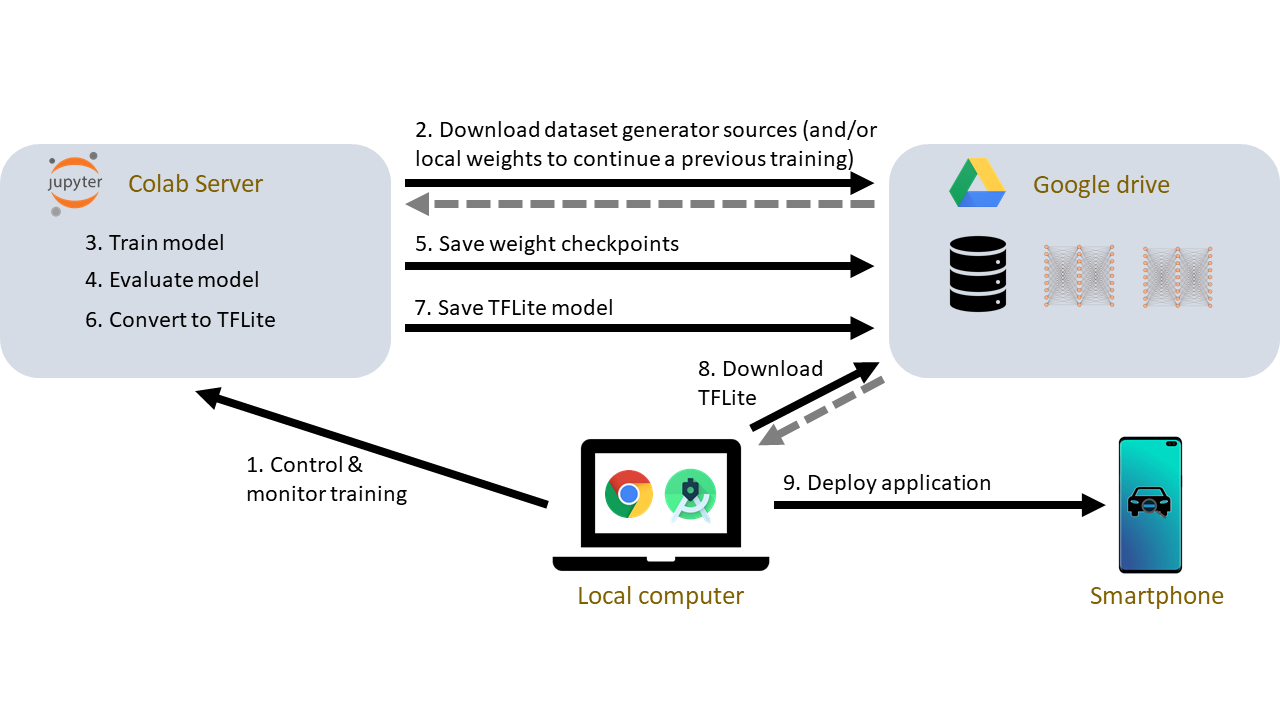
\includegraphics[width=1.0\columnwidth]{.//Figure/Technologies/training_environment.png}}
 \caption{High-level overview of a session in the training environment.}
 \label{fig:training_environment}
\end{figure}

Primarily, I monitored the training on TensorBoard, which shows a dashboard of the running session. After every epoch, the current model is evaluated. On these occasions, model checkpoints are saved (for early stopping and state preservation in case of a failure). After the training process, a standalone evaluation can be executed to verify the results and display the selected loss/protocol metrics.

The model can be saved in three different ways:

\begin{itemize}
  \item First, all the training files and checkpoints are zipped and saved to Google Drive.
  \item Second, only the latest (or the selected) checkpoint is preserved, and detailed log files are discarded (only metrics are retained like loss; model outputs for specific images are dropped) and saved to Drive.
  \item The third option is to convert the model to TFLite and save it.
\end{itemize}

\pagebreak
\section{Application}

I used the Kotlin programming language\cite{Kotlin} for the frontend and the backend. Kotlin is a statically typed, cross-platform language with type inference. In addition to the object-oriented approach, it also contains functional programming tools.

\subsection{Frontend}

Android provides an extensive application development ecosystem. I used the AndroidX namespace elements, which replaced the previous Support Library since Android 9.0. It is part of Android Jetpack, a collection of components for which the platform promises long-term support. The application extensively uses the CameraX API to manage device cameras. The ViewModel component moderates between the user interface and the business logic. The app contains a relational database implemented by the Room Persistence Library, which provides an abstraction layer over SQLite to more robust database access. To boost user experience, I decided to use a text-to-speech engine to read aloud alerts (useful if a user wants notifications while driving or wants to hear how to use tips).

Material Design defines guidelines for building the interface to maximize user experience. On Android, Material elements supported by the platform can be accessed through a library. The application uses its concepts, styles, icons, fonts, and UI elements (e.g., Floating Action Button, Snackbar).

\subsection{Backend}

I used Ktor\cite{Ktor} for the backend. It is an open-source, asynchronous framework for creating microservices and web applications. JSON data handling was implemented with the Gson library. I tested the server API with Postman, and for web scraping, I used ParseHub.


%----------------------------------------------------------------------------
\chapter{Sequential modeling}

This chapter focuses on the theoretical background of processing sequential data. As relatively simple deep learning-based solutions are surprisingly good with sequential data, I concentrate on neural network-based approaches.

Sequential modeling is a powerful way to solve numerous tasks, like video processing, time series prediction, or natural language processing. Many tasks can be modeled sequentially. The key is to project the domain problem to the proper abstraction. The categorization is partly based on source \cite{SequentialLecture}. There are different types of sequential tasks:

\begin{itemize}
  \item Vanilla approach processes the input in a \textit{single-input-single-output} (SISO) manner: for example, one frame of a video is classified independently of others. This is the case when the model has a single input image and makes classification.
  \item In a \textit{single-input-multiple-output} (SIMO) model, there is a single input and multiple possible outputs. For example, when an image contains multiple characters, the input is a single image, and the output is the sequence of characters in it.
  \item \textit{multiple-input-single-output} (MISO) models receive multiple inputs and output a single prediction. For example, the inputs are words of a textual review, and the prediction is the writer's sentiment.
  \item \textit{multiple-input-multiple-output} (MIMO) models receive multiple inputs and predict multiple outputs. These approaches can be divided into further subcategories:
    \begin{itemize}
     \item Some models receive multiple inputs and immediately output the prediction based on that. In video classification, a model usually receives multiple frames and outputs the class for each time frame, but these are predicted simultaneously, depending on each other.
	   \item In another configuration, popular in machine translation, models receive an input text and predict the current translated text on the fly, based on the current input. Here, input and output sequences are shifted relative to each other (some input characters are needed for the first prediction). For example, Google Translate is a model of this kind.
    \end{itemize}
\end{itemize}

A summary of the different tasks is illustrated by Figure \ref{fig:task_types}. Sequential data can be processed with different network types. In the following sections, I present these variants.

\begin{figure}[htb]
 \centerline{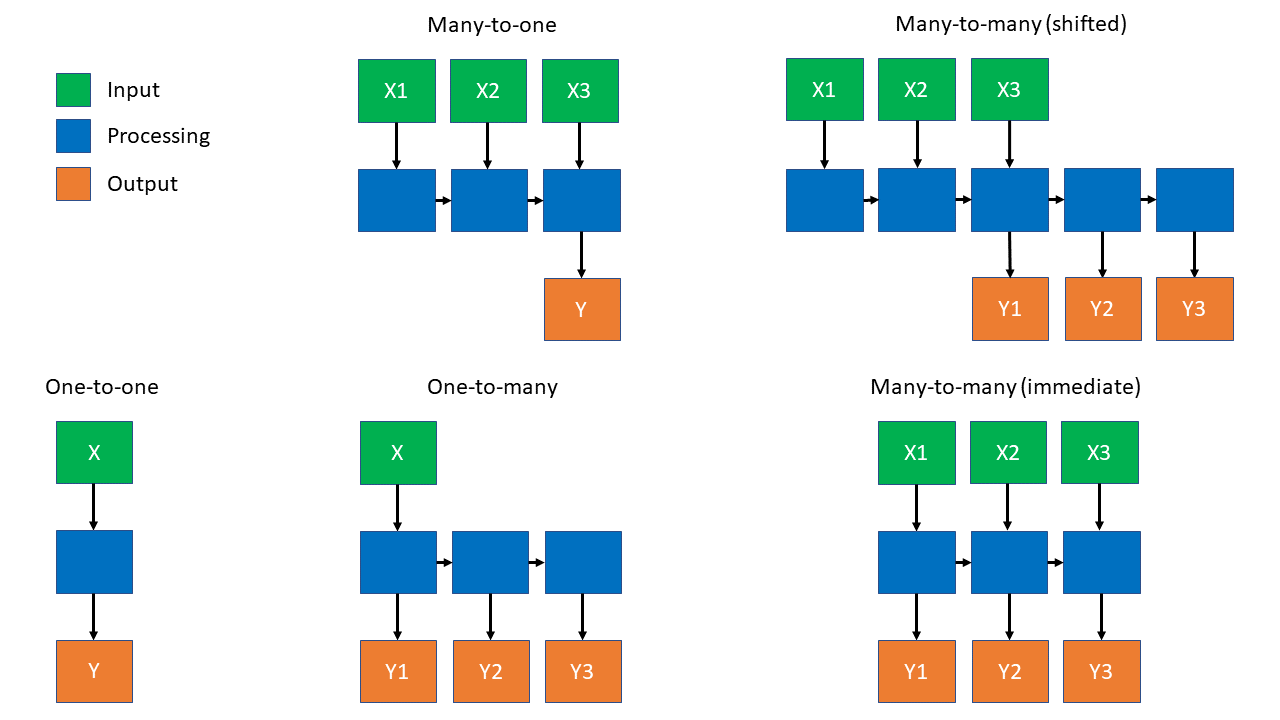
\includegraphics[width=1.0\columnwidth]{.//Figure/Sequential/task_types.png}}
 \caption{The different types of sequential tasks.}
 \label{fig:task_types}
\end{figure}

\section{One-dimensional convolution}

One-dimensional convolution networks can solve sequential problems by applying convolution to the serial input. These approaches are popular for problems like time-series analysis or audio input processing. 

When applying 1D convolution, the corresponding layer only sees the input in slices of the same width as the convolutional kernel. Pooling or strided convolution can be applied to reduce the length of the sequence, thus increasing the visible part of the input toward the deeper convolutional layers. Another approach uses \textit{dilated convolution}, where the kernel is inflated by inserting holes between its elements (Figure \ref{fig:dilated_convolution}). Dilation rate defines how much the kernel is widened. WaveNet\cite{WaveNet} is a successful dilated convolution-based MIMO model for sample-level audio synthesis. Its main data processing idea is illstrated by Figure \ref{fig:WaveNet_dilation}.

\begin{figure}[H]
 \centerline{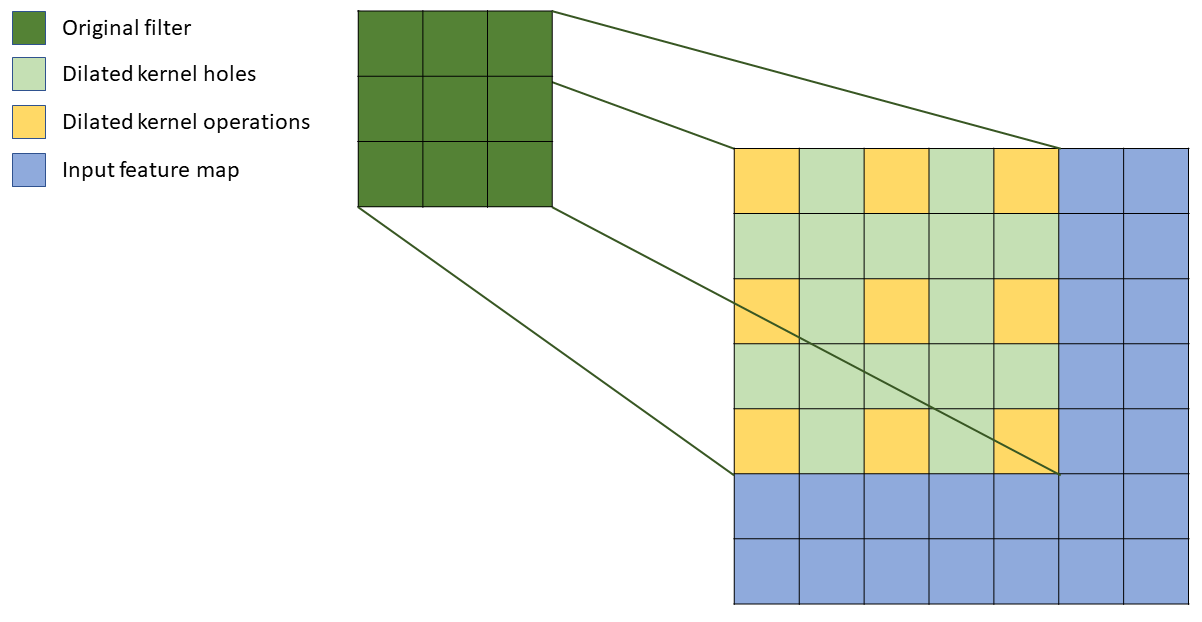
\includegraphics[width=0.8\columnwidth]{.//Figure/Sequential/dilated_convolution.png}}
 \caption{Two-dimensional dilated convolution.}
 \label{fig:dilated_convolution}
\end{figure}

\begin{figure}[H]
 \centerline{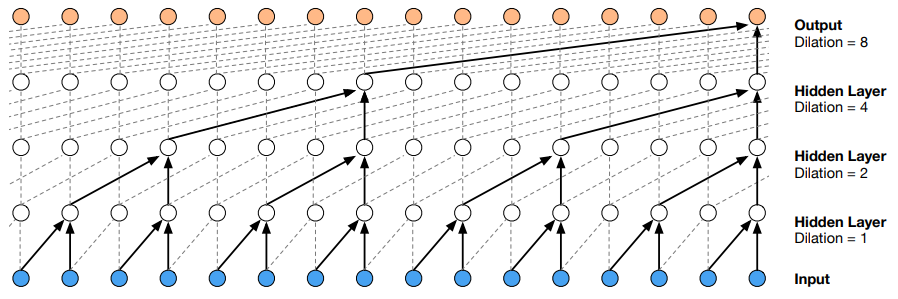
\includegraphics[width=1.0\columnwidth]{.//Figure/Sequential/WaveNet_dilation.png}}
 \caption{Stack of one-dimensional dilated convolutional layers in WaveNet. Source: \cite{WaveNet}}
 \label{fig:WaveNet_dilation}
\end{figure}

These models use solely convolutional layers, thus being relatively simple. While training, the simple backpropagation algorithm is used, and their runtime is only constrained by the convolution operation: in the case of two dimensions, if the input size is ${n}\times{n}$ and the kernel size is ${m}\times{m}$, the runtime is $\mathcal{O}({n^2}\times{m^2})$. However, these models lack one crucial element to process long sequential inputs: memory.

\section{Recurrent neural networks}

Classical neural networks are directed acyclic graphs (DAG), which define computational nodes and their connections. \textit{Recurrent neural networks} (RNN) are dynamic models containing recurrent links (directed loops). These connections can model an inner/hidden state (memory), which makes them useful when sequential data is processed, where later values depend on earlier ones. In every time step, the same function is called, meaning that the RNN's nodes and weights are the same. Figure \ref{fig:RNN} represents the inference steps of an RNN. These models do not require prior knowledge of the input data, and they are generally robust to noise\cite{CTC}. The section below discusses how such a network is trained.

\begin{figure}[htb]
 \centerline{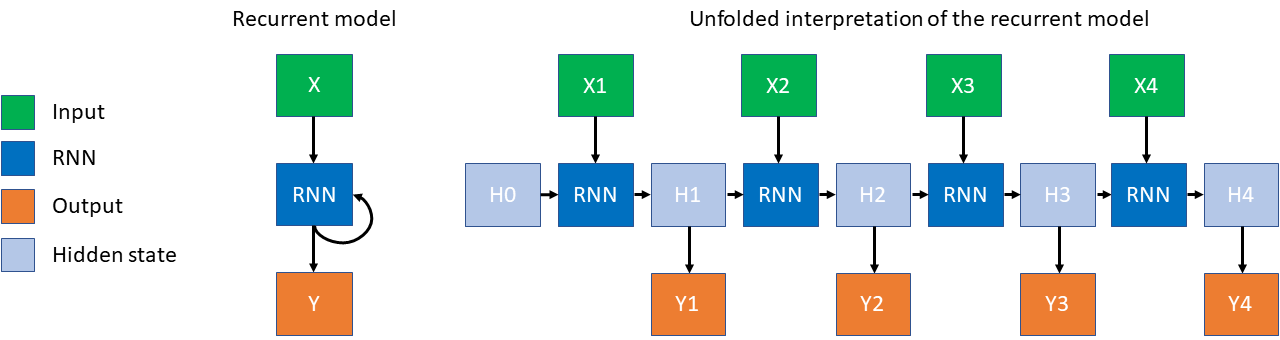
\includegraphics[width=1.0\columnwidth]{.//Figure/Sequential/RNN.png}}
 \caption{Unfolded interpretation of the RNN for a length-4 sequential input.}
 \label{fig:RNN}
\end{figure}

\subsection{Backpropagation through time}

In the classical backpropagation, a model input is first propagated forward the network, resulting in a prediction. When training the network, it is known what is expected from the model's output (ground truth). The difference between the prediction and the ground truth is calculated by the loss function, which results in the network's error. The error is then propagated backward the network: for each connection, a gradient is calculated based on how much it contributed to the local error of the following node. When each link has this value, the algorithm updates each connection weight based on its gradient and the learning rate.

Backpropagation through time\cite{SequentialLecture} (BPTT) works similarly. The difference is that the RNN is handled as an unfolded model. For each time step, the backpropagation algorithm is applied in a manner that the input of the \textit{Nth} step is the output of the \textit{N-1th} step (this wording is intentional, as we are moving backward in time). Gradient values are calculated for the whole network independently for each time step. When gradients are computed for a step, values are updated for each weight (Figure \ref{fig:BPTT}).

\begin{figure}[htb]
 \centerline{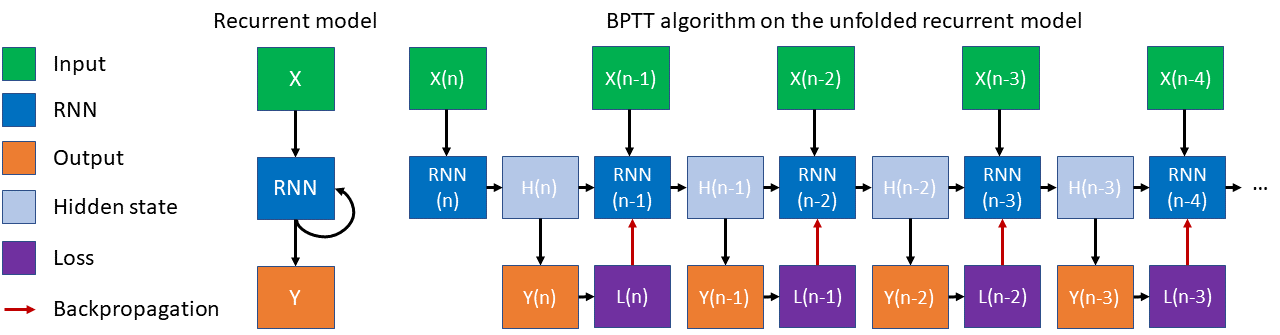
\includegraphics[width=1.0\columnwidth]{.//Figure/Sequential/BPTT.png}}
 \caption{Operation of the BPTT algorithm on the unfolded RNN.}
 \label{fig:BPTT}
\end{figure}

Usually, there is a truncation in the BPTT algorithm: the backward calculation only goes back to the last \textit{K} steps on the network unfolded by time. Otherwise, in the case of long series, the algorithm would take a lot of computational resources, significantly slowing down the training process.

\subsection{Limitations}

Many time steps are needed to create long-term inner memory. During BPTT, the error propagates back to these time steps on the same model. It means that we multiply the model's weight matrix multiple times, which is prone to the following problems:

\begin{itemize}
\item When the weight matrix singular value is high, it leads to gradient exploding. The weight updates are too big, so the model cannot converge.
\item When the weight matrix singular value is low, gradient vanishing happens. In this case, the gradients are too close to zero; weight updates are too small to improve the model.
\end{itemize}

For gradient exploding, possible solutions can be using saturating nonlinear activation functions or gradient clipping, where the values cannot go above a maximum. Skip connections can somehow compensate for the gradient vanishing problem, through which the error can flow freely back to the earlier time steps. However, these are not complete solutions.

\subsection{Long short-term memory}

Long short-term memory\cite{LSTM} (LSTM) is a type of RNN cell which uses a gated approach. It implements a short-term memory that can be long enough to handle longer sequences than simple RNNs can do. An LSTM cell has three inputs in each time step:

\begin{itemize}
\item \textit{C}: The cell state is the interpretable, optimized output of the cell.
\item \textit{H}: Hidden state, which is the inner state of the LSTM block.
\item \textit{X}: Input tensor, the input from the earlier network layers (for example, a feature map created by convolutional layers which we want to process sequentially, from left to right).
\end{itemize}

There are multiple trainable gates within an LSTM cell, manipulating the signal flow and thus modeling what information is needed from a specific input given a state. These gates are trainable to model memory. The gates are the following:

\begin{itemize}
\item \textit{forget}: Responsible for deleting certain things from the cell state based on the fused input of the hidden state and the input tensor. This gate was not part of the initial publication; it was added a few years later\cite{LSTM-ForgetGate}. Forget gate allows the cell to reset its state and was crucial to the success of LSTM.
\item \textit{input}: Decides what items of the fused input should be written to the cleaned cell state.
\item \textit{gate}: Applies nonlinearity to the fused input written to the cell state. This is the only gate that uses the tanh activation function instead of the sigmoid. This gate projects the values between [-1, 1] to provide the necessary abstraction switching of the signal while maximizing the output range, retaining the saturating behavior. The other gates use sigmoid activation because they mask the signal to be retained (where the minimum is 0 and the maximum is 1).
\item \textit{output}: Masks the hidden state output derived from the cell state.
\end{itemize}

In an LSTM cell, there are only saturating nonlinear activation functions, which can handle the gradient exploding problem. There is no activation function between the input and the output cell state, only one multiplication (forget gate) and one addition. This means that the input signal can propagate to the output without severe decrease, and thus the gradients can backpropagate without downscaling. This path forms a gradient highway across the unfolded model (containing the same LSTM cell of each time step) during BPTT training. This path is essential in solving the gradient vanishing problem induced by the numerous time steps. The visual representation of an LSTM cell is illustrated by Figure \ref{fig:LSTM}.

\begin{figure}[htb]
 \centerline{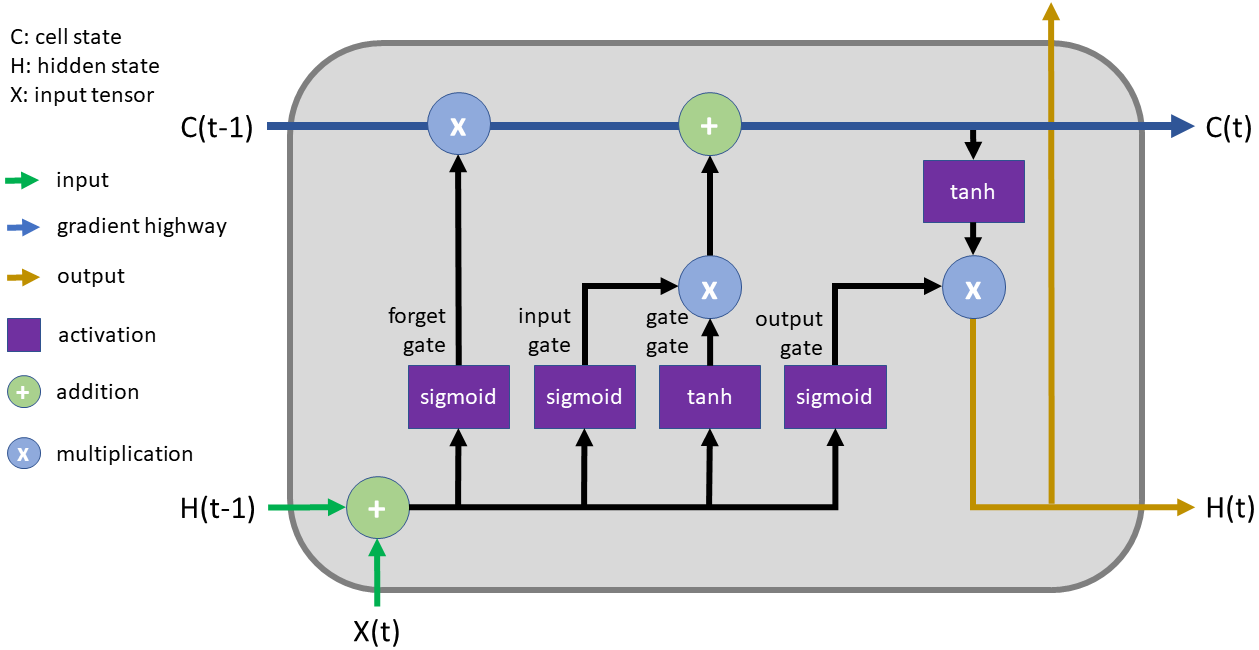
\includegraphics[width=1.0\columnwidth]{.//Figure/Sequential/LSTM.png}}
 \caption{Inner structure of an LSTM cell.}
 \label{fig:LSTM}
\end{figure}

LSTM is a relatively old approach from 1997, a mature standard tool for solving sequential problems. Over time, other solutions have emerged, such as the Gated Recurrent Unit\cite{GRU} (GRU) from 2014, which similarly models memory, but with fewer parameters (three gates instead of four). I decided to present LSTM because it is easier to understand thanks to its well-separated elements.

\section{Connectionist Temporal Classification}

RNNs are good at sequence learning, but they require thoroughly segmented and labeled data, which is time-consuming. Traditional loss functions like mean squared error cannot work well without properly segmented data because they assume that each item in the sequence is independent. This leads to limited model applicability.

Connectionist Temporal Classification\cite{CTC} is a loss function to handle sequential input, which is noisy and unsegmented. It assumes that the network output is a conditional probability distribution over the label sequences. This way, the loss function transforms the sequential problem into classification, where the model needs to select the most probable label for a given input sequence. 

\subsection{Example}

I illustrate the function's applicability on an example with an input image in which we want to read a text. This example is partly based on \cite{CTCexp}. Reading the text in the image can be modeled as a sequential problem, where we want to process the picture from left to right. Only the input and the ground truth text label are needed when training with CTC. We discard the information where the particular characters are. CTC tries the possible alignments of the ground truth label in the image and sums all the scores. This way, it does not matter where the text is in the picture - the algorithm could find a suitable label alignment when the match value is high. This value should be maximized to the alignments outputting the ground truth label.

Because CTC tries to find the optimal label alignment, a good character encoding is needed to help distinguish good and bad ones. The characters are separated by a blank token (marked as ``|''), which separates the letters. This way, when a wide character is processed and triggers multiple predictions next to each other, we can merge them between the blank tokens to identify the actual letter. This also solves the problem of segregating the same characters next to each other. The encoding approach makes it possible to represent the same text multiple ways, allowing different alignments to match. The neural network is trained to predict the output in this encoded format.

\begin{itemize}
\item The word ``of'' is recognized when the output is ``|o|ff|'', ``|oooooo||||ffff||||'', or ``o|f''.
\item The word ``off'' is recognized when the output is ``||oo|f||f'', ``|ooo|fff|f|'', or ``o|f|f''.
\end{itemize}

To calculate the scores for an alignment, we have to consider all the possible paths and sum the ones producing the same decoded text. The added up probability is the overall score of the path. Each path text is then compared to the ground truth label, and the loss value is calculated weighted by the path probabilities. The loss function needs to be minimized. For that, CTC uses the negative sum of the log probabilities. The probability is maximized when this loss is minimized, so the function motivates the model to find good predictions.

The model outputs a matrix containing a score for each character at each time step. There are different approaches to decode this matrix. One method is called \textit{best path decoding}, where:

\begin{itemize}
\item The algorithm takes the maximum prediction at each step, producing the most probable path.
\item To decode the prediction, the same characters are removed next to each other, then the blank tokens are also removed. The remaining output is the predicted text.
\end{itemize}

This method is fast and usually good, but it is just an approximation. There are different decoding approaches where multiple paths can be considered (similarly when calculating the CTC loss for the different paths). One other algorithm is Word Beam Search\cite{WordBeamSearch}, where the number of nodes to consider at each time step can be defined. It can make decoding more accurate but also scalable.
%----------------------------------------------------------------------------
\chapter{Object detection}

In this section, I discuss the work done related to object detection. In addition to the model development phases, I also describe the related research. Since deep learning requires a greater theoretical background, I assume knowledge of its general principles (backpropagation, convolutional neural networks) for reasons of length. I describe the theoretical background related to object detection in detail.

\section{Related Work}

\section{Data}

\section{Model}

\section{Evaluation}
%----------------------------------------------------------------------------
\chapter{Automatic license plate recognition}

Automatic license plate recognition (ALPR) refers to a technology that identifies vehicles based on their number plates. It is based on Optical character recognition. Traditionally, these systems are used to find stolen vehicles, check for road usage permits, measure vehicle speed, or operate parking garages. The technology is also suitable for tracking vehicles and collecting location data. This may be to the benefit of the authorities, but in Europe, it raises privacy concerns, as drivers have the right to data privacy.

ALPR systems can be categorized according to several aspects. There are fixed (pre-installed) and mobile (cameras in vehicles) systems based on their mobility. According to another aspect, some systems perform on-device image evaluation, while others process them remotely (like on a central computer or a server farm). Both solutions have pros and contras in terms of network bandwidth- and hardware requirements.

\begin{figure}[htb]
 \centerline{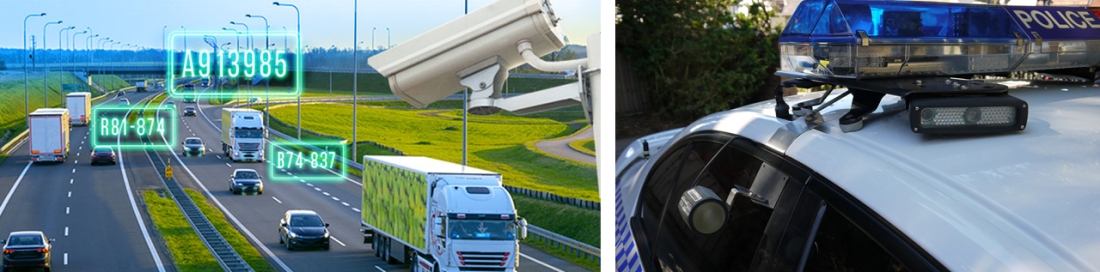
\includegraphics[width=1.0\columnwidth]{.//Figure/ALPR/alpr-systems.png}}
 \caption{Pre-installed closed-circuit ALPR system\cite{ImageFixedALPR} (left) and a police car equipped with mobile ALPR\cite{ImageMobileALPR} (right).}
 \label{fig:simple}
\end{figure}

\section{History}

The technology began to spread worldwide in the 2000s; however, the first ALPR systems were in service as early as the late 1970s. The first system was created in 1976 in the UK by the Police Scientific Development Branch. Their solution has been installed to monitor the A1 road’s traffic and to look for stolen vehicles. The first arrest based on ALPR identification of a stolen car happened in 1981\cite{ANPR_history}.

As the technology evolved, more sophisticated solutions emerged. Fixed cameras began to form coherent networks, and thanks to hardware developments, previously expensive and cumbersome systems became affordable and widely available. The proliferation of the systems was further facilitated by changing license plates in many countries (like in the Netherlands) to help ALPR operation\cite{DutchLicensePlates}.

During the 1990s, mobile ALPR systems also appeared. This was due to the elimination of special hardware requirements, and the more robust solutions no longer required certain view angles or conditions to work. A challenging task, in this case, is solving the power supply requirements of the hardware from a battery. Providing an internet connection while moving is also a requirement. These have been challenging issues in the past; nowadays, they are no longer limiting factors.

\section{Components}

There are many versions of ALPR solutions that regularly differ from each other. Still, below I try to give a general picture of what image processing tasks arise in an ALPR system\cite{ANPR} (without claiming completeness):

\begin{itemize}

\item Plate localization is the process of finding and isolating the license plates. This can be either done with object detection or semantic segmentation.

\item Plate resizing and orientation try to minimize the skew of an image and adjust the dimensions to the required size. Various heuristics (like Projection Profile Method\cite{ProjectionProfileMethod}) exist to determine skew and apply projection afterward. A recent solution is the use of attention-based transformer neural networks\cite{SpatialTransformerNetworks}.

\item Image manipulation is a collective concept for pixel-level transformations based on its statistical properties in the present work’s context. The process can either be normalization (rescale values into a range of [0, 1]), standardization (rescale values to have 0 mean and a standard deviation of 1), grayscale conversion, a combination of these, or other. Care must be taken with these operations because the image quality significantly affects the effectiveness of subsequent steps.

\item Optical character recognition consists of character segmentation and classification - more about this in the OCR chapter.

\item Syntactic inspection is the process where country-specific information is taken into consideration (position of specific characters, length of the recognized sequence). The goal here is to extract and validate the correct identifier.

\item Averaging multiple images can significantly improve performance. It helps by averaging unwanted protruding effects, such as blur or reflection, that often occur in pictures of moving vehicles.

\end{itemize}

Not all ALPR systems explicitly separate the above points (for example, the OCR character segmentation- and classification can be done at once or as separate steps). These factors influence the usability of a solution - the key is the implementation and coordination of them.

\section{Challenges}

In the case of an ALPR system, there are numerous difficulties for which there are different solutions.

The variance of the images is quite large. Accurate operation at different times (day or night) and weather conditions (sunny, snowy, foggy, rainy) is also expected in most cases. Image manipulation techniques can overcome this problem to some extent. Devices can see the license plates in different sizes and angles depending on their installation. This is where plate localization, then proper resizing and orientation can help - although this cannot provide a solution for too distant, low-quality license plate images. Blurring caused by the movement of cars is also a problem. The answer to this is to use short-shutter cameras (~1/1000 second) with a global shutter. Modern smartphones are generally capable of the required shutter speeds. However, the presence of the rolling shutter can still be an issue.

\begin{figure}[htb]
 \centerline{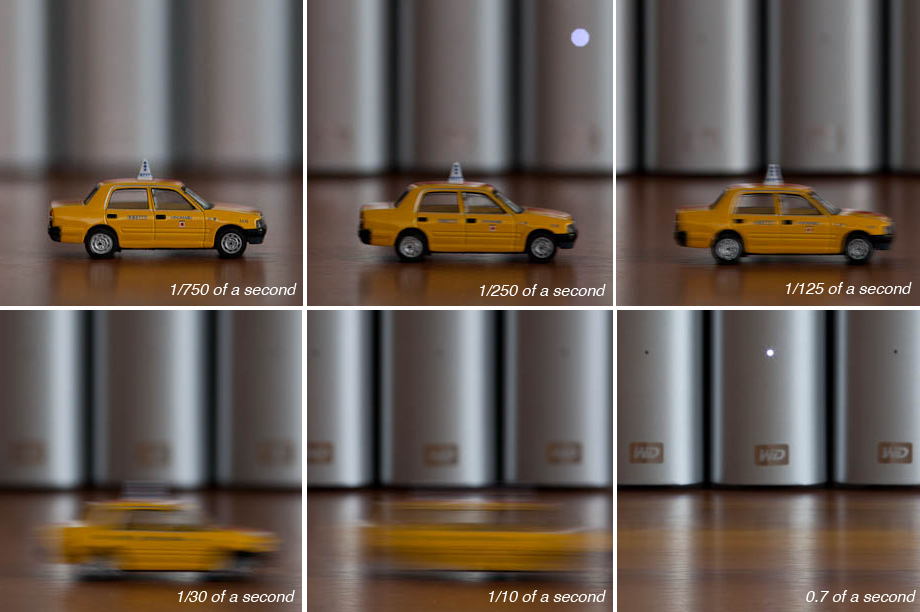
\includegraphics[width=1.0\columnwidth]{.//Figure/ALPR/shutter-speed.png}}
 \caption{The effect of shutter speed illustrated by a model car\cite{ShutterEffect}.}
 \label{fig:simple}
\end{figure}

Another common difficulty is the variety of number plates. License plates can have various structures, colors, and fonts, and their shape can also vary. It is typical for single and multi-row license plates to be used within a country. For these reasons, most of the current ALPR systems can only be used satisfactorily in a given country. However, the situation in Europe has improved in recent years with the proliferation of EU number plates. Although ALPR processability is now considered in the design of most license plates, in some countries, few characters have almost the same symbol (like 0 and O in England). Outside of Europe, characters outside the Latin alphabet may also appear. Character variability is discussed in more detail in the OCR chapter. Dirt may also be present on license plates, or other objects may obscure their text. Deliberate circumvention attempts can be an additional difficulty for ALPR systems. This can be, for example, covering certain characters or using a surface that impairs visibility. I am not addressing this issue in this work.

\section{Evaluation}

Most ALPR system publishers provide rough metrics about their solutions, making it difficult to compare them. I found two de-facto benchmark datasets for this task. The first is the SSIG SegPlate Database\cite{SSIG-ALPR}, with 101 on-track vehicles captured by a static camera. The other is the UFPR-ALPR Dataset\cite{UFPR-ALPR}, containing 4,500 images with 30,000 number plate characters.

\begin{figure}[htb]
 \centerline{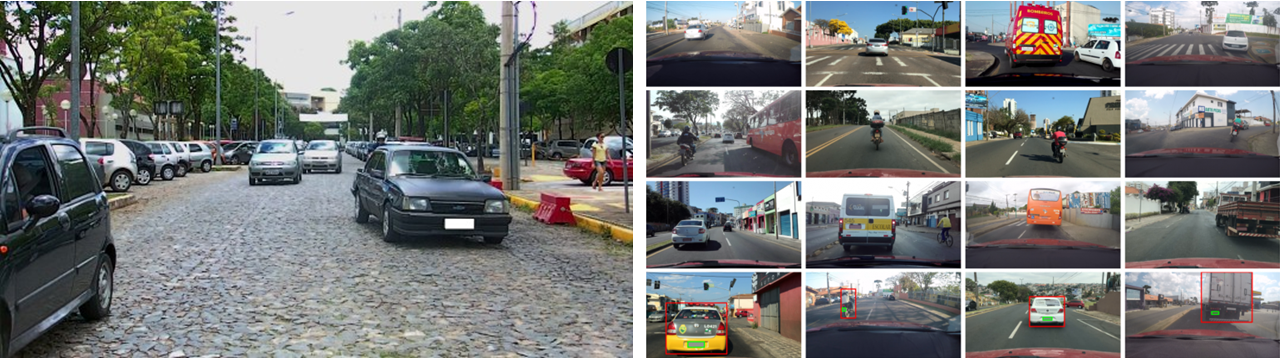
\includegraphics[width=1.0\columnwidth]{.//Figure/ALPR/alpr-datasets.png}}
 \caption{Samples from the SSIG SegPlate\cite{SSIG-ALPR} (left) and the UFPR-ALPR\cite{UFPR-ALPR} (right) datasets.}
 \label{fig:simple}
\end{figure}

Sighthound\cite{Sighthound} and OpenALPR\cite{OpenALPR} are considered to be widespread market players. These solutions have been compared to a YOLO-based ALPR system in the following publication\cite{RobustRealTimeALPR_YOLO}. Based on their performances on the SSIG dataset, Sighthound had 89.80\%, OpenALPR 93.03\%, and YOLO-ALPR 93.53\% of accuracy. On the more challenging UFPR-ALPR dataset, Sighthound scored 47.39\%, OpenALPR 50.94\%, and YOLO-ALPR 64.89\% of accuracy.


%----------------------------------------------------------------------------
\chapter{License plate localization}

This chapter discusses the work done on vehicle and number plate detection. The main goal of this section’s algorithm is to localize number plates on input images. I used deep learning-based object detection for this task. I chose object detection over semantic segmentation because multiple license plates on a single image can be possible. Semantic segmentation does pixel-level classification, thus does not help in distinguishing objects of the same class. Object segmentation would hardly constrain the maximum number of things to find in the same type on the image.

Although the main task is number plate detection, I also decided to include vehicle detection. License plates are usually on vehicles that we want to identify. They have properties like type, make and color. If a stolen number plate is identified, we are primarily interested in the vehicle it belongs to. We can also infer additional information (like number plates without vehicles, which are false positives) by doing vehicle detection.

\section{Data}

The following section describes collecting, analyzing, cleaning, and validating the dataset needed for training. An essential aspect of obtaining the data was to cover as many images as possible with labeled license plates. Thousands of photos are necessary to ensure proper data diversity. The aim was to get not only license plate annotations but also vehicle annotations.

\subsection{Sources}

There were not many standalone datasets meeting these requirements. I conducted my research mainly on Kaggle and the Google Dataset Search engine. The most promising sets had only a few hundred labels.

I examined the Common Objects in Context\cite{MS-COCO} (COCO) and the Open Images\cite{OID} (OID) datasets. These are large sets containing 123,287 and roughly 2 million detection images. I assumed that if at least one of them had license plate annotations, the number of these labels would be enough. Of these, OID has a vehicle registration plate class. As the dataset is huge, I used a Python toolkit to download all the 6,867 images containing these items. I also downloaded all the detection annotations in separate CSV files (OID train, validation, test). The total size of all files was 2.352 GB.

\subsection{Pre-processing}

The application is not limited to detecting only cars. It is necessary because the stolen vehicle database and the police data source contain cars, trucks, motorbikes, and other vehicles.

All the annotations of the downloaded images were kept. OID has a hierarchical class structure from which I chose nine classes representing the new vehicle class (car, airplane, helicopter, boat, motorcycle, bus, taxi, truck, ambulance). I discarded the original OID vehicle class because it contained objects challenging to place in other subclasses like surfboards and wheelchairs. A few less essential types were discarded (like aerial vehicles or snowmobiles) to keep the cardinality of the resulting classes equal. Figure \ref{fig:OID_classes} shows all the classes used from the OID Vehicle branch.

\begin{figure}[htb]
 \centerline{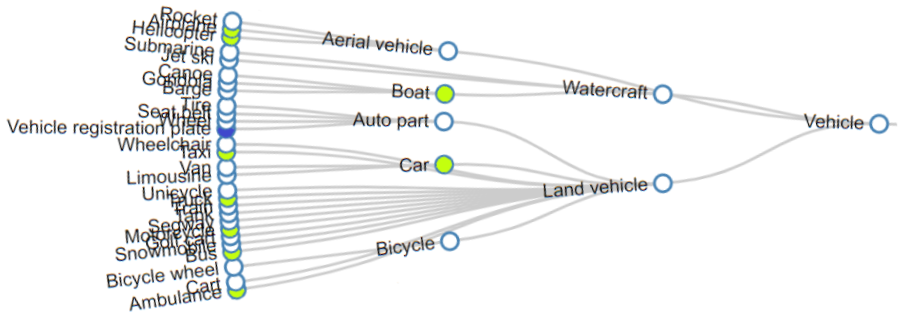
\includegraphics[width=1.0\columnwidth]{.//Figure/PlateLocalization/OID_classes.png}}
 \caption{Selected classes from the original OID Vehicle branch: \textcolor{blue}{license plate}, \textcolor{green}{vehicle}.}
 \label{fig:OID_classes}
\end{figure}

\subsection{Analysis}

I used Power BI to analyze and visualize the downloaded content. My project uses CSV files as data sources. The raw dataset contains 6,867 images with 28,102 bounding boxes, roughly four annotations per image. There are 9,934 vehicle registration plate annotations, one-third of all the boxes. The report revealed that the average image size is $1005\times753$ pixels. While most images have a dimension of $1024\times768$ pixels, some exemptions occur. As the model input is always resized, this is not important to examine more thoroughly.

Table \ref{tab:class_multiplicity} and Figure \ref{fig:class_multiplicity} show that there are more vehicle boxes in the dataset. The left chart shows cardinalities compared to each other, while the right one corresponds to cardinalities relative to the number of images.

\begin{table}[H]
 \caption{Multiplicity of class boxes (left) and the number of images in which a class is present (right).}
 \label{tab:class_multiplicity}
\begin{minipage}{.5\linewidth}
 \centering
\begin{tabular}{ll}
    class & box cardinality\\ \hline
    vehicle & 18,168 \\
    vehicle reg. plate & 9,934 \\
    \textbf{total} & \textbf{28,102} \\
\end{tabular}
\end{minipage}%
\begin{minipage}{.5\linewidth}
 \centering
\begin{tabular}{ll}
    class & image cardinality\\ \hline
    vehicle & 5,806 \\
    vehicle reg. plate & 6,867 \\
    \textbf{total} & \textbf{6,867} \\
\end{tabular}
\end{minipage} 
\end{table}

\begin{figure}[H]
 \centerline{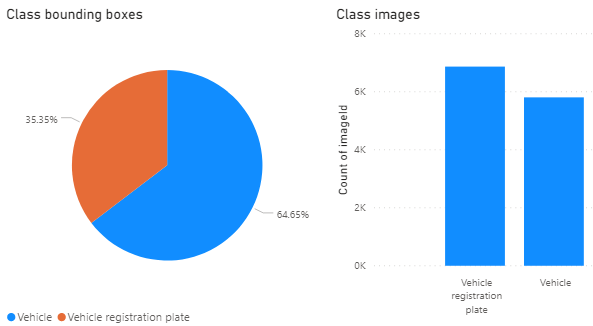
\includegraphics[width=1.0\columnwidth]{.//Figure/PlateLocalization/class_multiplicity.png}}
 \caption{Multiplicity of class boxes and the total number of images per class.}
 \label{fig:class_multiplicity}
\end{figure}

Table \ref{tab:dataset_box_properties} and Figure \ref{fig:median_avg_boxes_plates} show the average bounding box dimensions for license plates. They occupy an average of 10\% of the x-axis and 5\% of the y-axis, which means the detector needs wider anchor boxes of this size. The average number plate box is an elongated rectangle, confirming that the data looks like it should (both vehicles and number plates are usually wider along the x-axis).

\begin{table}[H]
\caption{Dataset box properties.}
\label{tab:dataset_box_properties}
\noindent
\centering
\begin{tabular*}
{\columnwidth}{@{\extracolsep{\stretch{1}}}*{5}{r}@{}}
    type & X\textsubscript{min} & X\textsubscript{max} & Y\textsubscript{min} & Y\textsubscript{max}\\ \hline
    median & $0.41$ & $0.58$ & $0.60$ & $0.68$ \\
    average & $0.44$ & $0.55$ & $0.58$ & $0.65$ \\
\end{tabular*}
\end{table}

\begin{figure}[H]
 \centerline{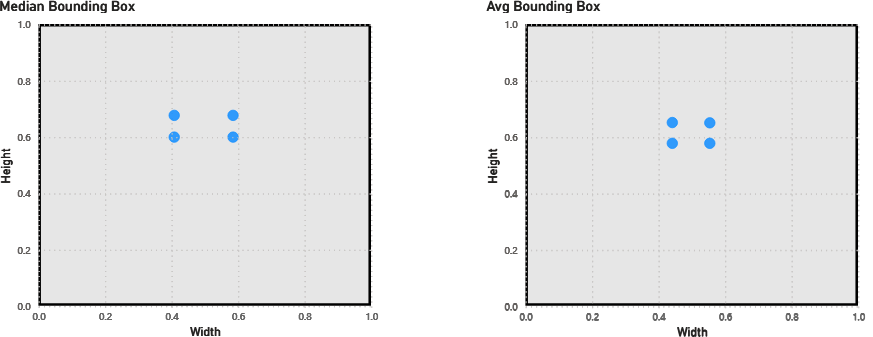
\includegraphics[width=1.0\columnwidth]{.//Figure/PlateLocalization/median_avg_boxes_plates.png}}
 \caption{Median and average bounding boxes of license plates.}
 \label{fig:median_avg_boxes_plates}
\end{figure}

OID has a separate train, validation, and test set. It turned out that they differ in bounding box position distributions, and there is also a slight difference in the average box numbers per image (4.09 vs. 3.33). As the average license plate is also bigger in the validation set, it may be misleading to compare the performance of the models based on that subset. I discovered the phenomenon when I was comparing the average boxes. The phenomenon is illustrated by Tables \ref{tab:avg_boxes_across_subsets} and \ref{tab:median_boxes_across_subsets} and Figure \ref{fig:median_avg_boxes_train_validation}. A closer look confirmed that some outliers did not cause it - the reason was the difference in the distribution of the box sizes across different subsets.

\begin{table}[H]
\caption{Average box coordinates across different subsets.}
\label{tab:avg_boxes_across_subsets}
\noindent
\centering
\begin{tabular*}
{\columnwidth}{@{\extracolsep{\stretch{1}}}*{5}{r}@{}}
    subset & X\textsubscript{min} & X\textsubscript{max} & Y\textsubscript{min} & Y\textsubscript{max}\\ \hline
    $train$ & $0.34$ & $0.65$ & $0.48$ & $0.70$ \\
    $validation$ & $0.21$ & $0.74$ & $0.27$ & $0.65$ \\
\end{tabular*}
\end{table}

\begin{table}[H]
\caption{Median box coordinates across different subsets.}
\label{tab:median_boxes_across_subsets}
\noindent
\centering
\begin{tabular*}
{\columnwidth}{@{\extracolsep{\stretch{1}}}*{5}{r}@{}}
    subset & X\textsubscript{min} & X\textsubscript{max} & Y\textsubscript{min} & Y\textsubscript{max}\\ \hline
    $train$ & $0.38$ & $0.61$ & $0.46$ & $0.66$ \\
    $validation$ & $0.32$ & $0.66$ & $0.32$ & $0.62$ \\
\end{tabular*}
\end{table}

\begin{figure}[H]
 \centerline{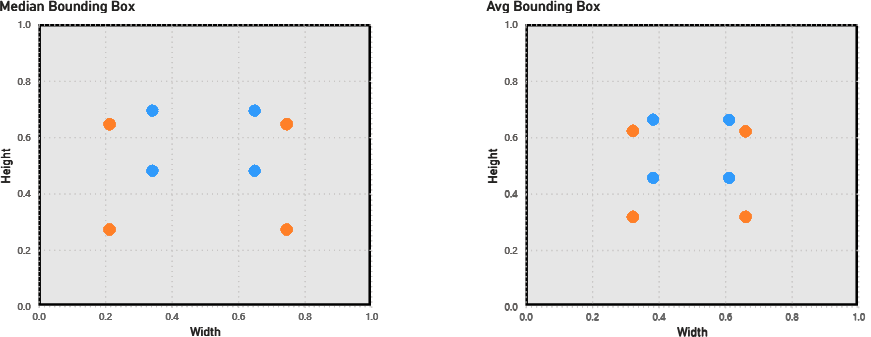
\includegraphics[width=1.0\columnwidth]{.//Figure/PlateLocalization/median_avg_boxes_train_validation.png}}
 \caption{Median and average bounding boxes of \textcolor{blue}{train} and \textcolor{orange}{validation} sets.}
 \label{fig:median_avg_boxes_train_validation}
\end{figure}
\newpage

I applied data aggregation and partition to fix this problem. First, all the images and annotations have been aggregated, then saved to TFRecord\cite{TFRecord} format. It is a binary file format that stores images and custom labels together. This format's main advantage is that it can be processed rapidly, which is not negligible if the dataset has thousands of instances. I created an encoder Python script to generate the dataset files. Detailed contents of such a record are shown below:

\begin{lstlisting}
features {
  feature {
    key: "image/encoded"
    value {
      bytes_list {
        value: binary encoded image
      }
    }
  }
  feature {
    key: "image/height"
    value {
      int64_list {
        value: 769
      }
    }
  }
  ...
  feature {
    key: "image/object/bbox/xmax"
    value {
      float_list {
        value: 0.800000011920929
        value: 0.3006249964237213
      }
    }
  }
  feature {
    key: "image/object/class/text"
    value {
      bytes_list {
        value: "Vehicle"
        value: "Vehicle registration plate"
      }
    }
  }
  ...
}
\end{lstlisting}

The dataset has been evenly sharded between 14 files using Euclidean division \textit{(n \% 14)}. While generating TFRecord batches, I created the corresponding CSV files to analyze later. I selected the validation and test batches, and all the other files became part of the training set. This way, the problem discussed above has been resolved. Table \ref{tab:avg_boxes_after_redistributing} shows the average bounding boxes of the test (12 batches), validation (1 batch), and train (1 batch) sets. They are almost identical.

\begin{table}[htb]
\caption{Average bounding boxes after redistributing the train, validation, and test sets.}
\label{tab:avg_boxes_after_redistributing}
\noindent
\centering
\begin{tabular*}
{\columnwidth}{@{\extracolsep{\stretch{1}}}*{5}{r}@{}}
    subset & X\textsubscript{min} & X\textsubscript{max} & Y\textsubscript{min} & Y\textsubscript{max}\\ \hline
    $train$ & $0.38$ & $0.61$ & $0.45$ & $0.66$ \\
    $validation$ & $0.39$ & $0.61$ & $0.47$ & $0.66$ \\
    $test$ & $0.38$ & $0.60$ & $0.47$ & $0.68$ \\
\end{tabular*}
\end{table}

\subsection{Evaluation}

The final dataset has 5,793 (84\%) training, 537 (7.8\%) validation, and 537 (7.8\%) test images. It has a 23,739 (84\%) training, 2,200 (7.8\%) validation, and 2,163 (7.7\%) test bounding box distribution. There are general dataset division guidelines (like the 70-20-10 rule), from which I deviated. In my opinion, the validation and test sets are already sufficiently representative after reshuffling them in the order of thousands; therefore, I tried to maximize the size of the train set. I created a TFRecord viewer script to validate image and annotation decoding. Figure \ref{fig:training_samples} and \ref{fig:validation_test_samples} show some samples from each subset.

\begin{figure}[H]
 \centerline{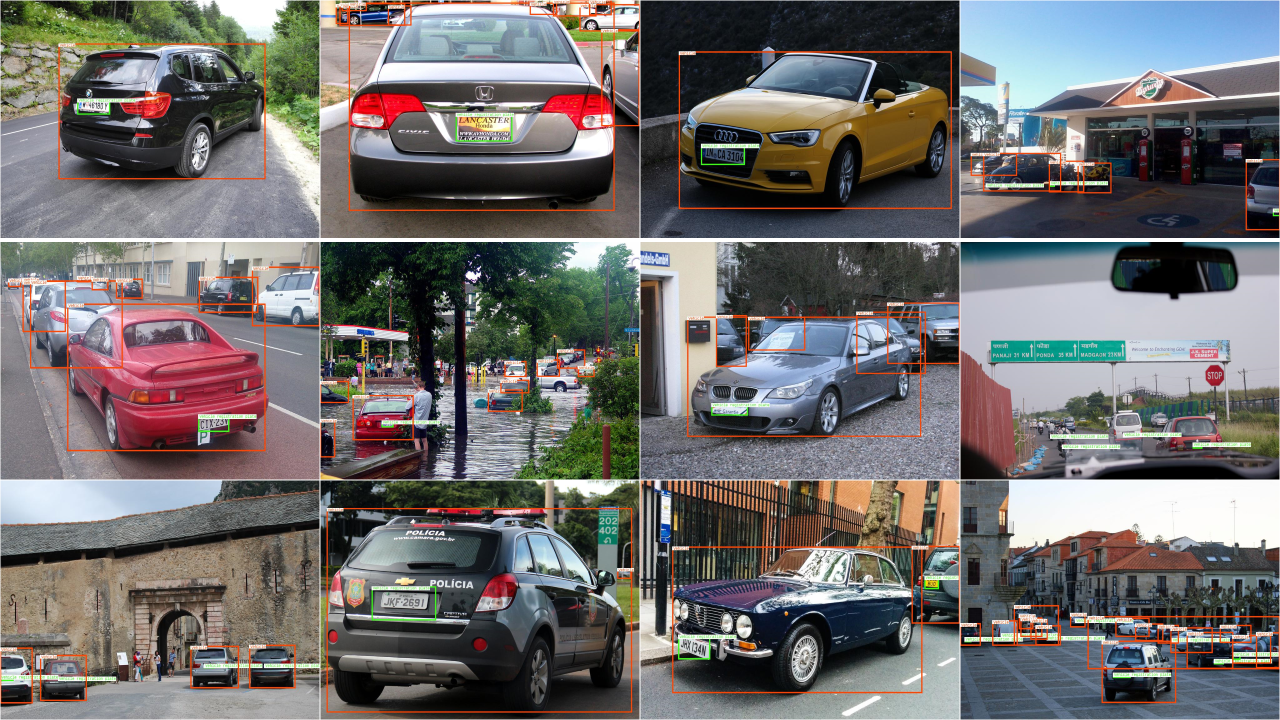
\includegraphics[width=1.0\columnwidth]{.//Figure/PlateLocalization/training_samples.png}}
 \caption{Training samples with bounding boxes: \textcolor{green}{license plate}, \textcolor{orange}{vehicle}.}
 \label{fig:training_samples}
\end{figure}

\begin{figure}[H]
 \centerline{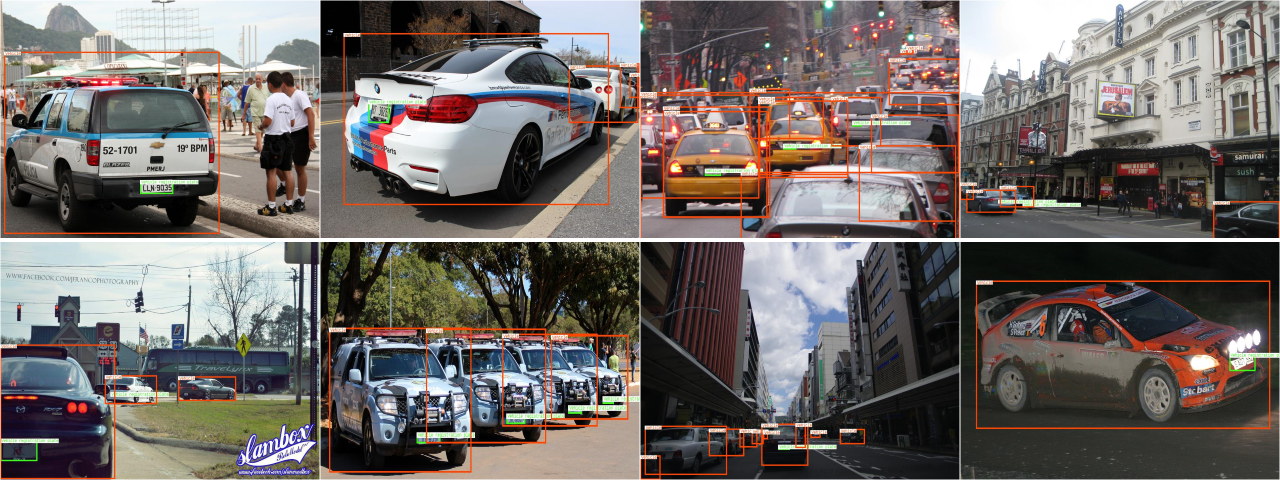
\includegraphics[width=1.0\columnwidth]{.//Figure/PlateLocalization/validation_test_samples.png}}
 \caption{Samples with boxes: \textcolor{green}{license plate}, \textcolor{orange}{vehicle}. 1st row: validation, 2nd row: test samples.}
 \label{fig:validation_test_samples}
\end{figure}

It is important to note that the dataset is not perfect - there are some inconsistencies. It turned out that some images were incompletely annotated. The problems can be categorized in two ways:

\begin{itemize}
  \item Visible license plates are not annotated (Figure \ref{fig:missing_labels} top left).
  \item Vehicle annotations are entirely missing (Figure \ref{fig:missing_labels} top right).
\end{itemize}

One more thing to spot: as a few original OID classes were discarded to keep the new vehicle class close to the cardinality of vehicle registration plates, some types of boxes (like vans) were dropped (bottom row of Figure \ref{fig:missing_labels}). This is partly the reason for some of the missing bounding boxes.

\begin{figure}[htb]
 \centerline{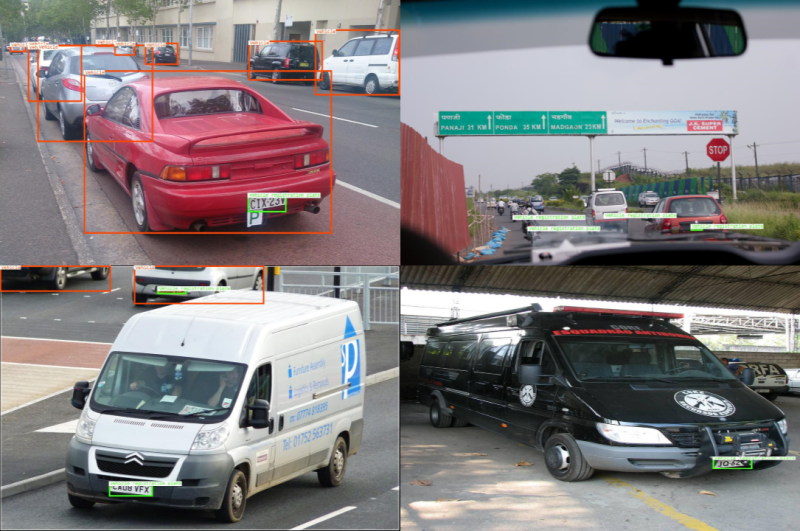
\includegraphics[width=0.8\columnwidth]{.//Figure/PlateLocalization/missing_labels.png}}
 \caption{Top row: inconsistently missing labels. Bottom row: no vehicle boxes around vans.}
 \label{fig:missing_labels}
\end{figure}

These are good examples that while the dataset may be appropriate for the task, it has its flaws. Since balancing classes relative to each other is a priority to avoid bias, I have not made further changes.

\section{Algorithm}

In the following part, I present the preliminary steps of model creation (choosing appropriate metrics), architecture selection, training and fine-tuning, and then post-production (quantization, wrapping).

I chose the COCO evaluation protocol mainly because it measures performance on different-sized objects. As discussed earlier, the vehicle registration plates are relatively small on the images, so I wanted to see how different sizes affect performance. In my opinion, OID would not have been suitable for this task because I would have lost size-specific indicators, but I would not have won with the class-level metrics because there are only two classes.

\subsection{Workflow}

Different data subsets have different roles during the development process. The main idea is to train models on the training set (with most images) and evaluate them on the validation set. When the best model is selected based on its validation performance, it is re-evaluated on an unknown test set to spot if overfitting occurs - which is the case when the model performs noticeably weaker on the new set. Sometimes, this type of overfitting happens as we select the best model based on the validation set – and it remains unnoticed if we do not apply this technique. I used the workflow with the different subsets outlined by Figure \ref{fig:subsets_workflow}.

\begin{figure}[htb]
 \centerline{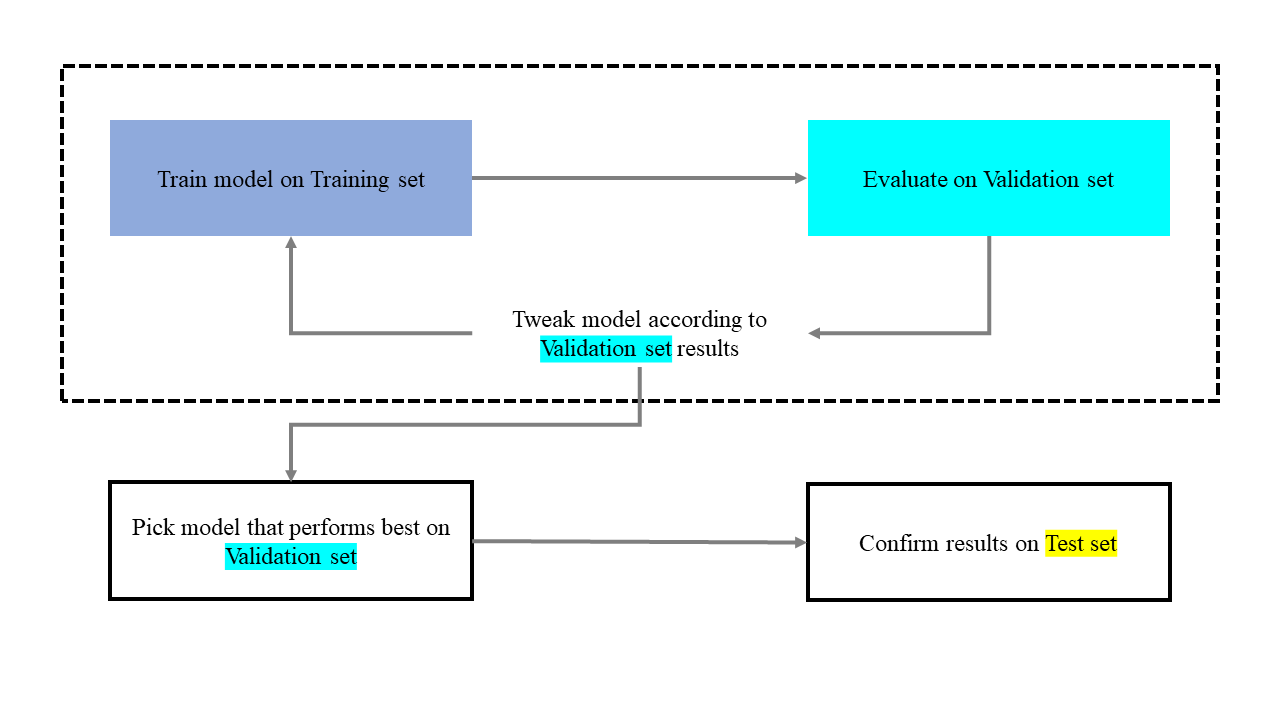
\includegraphics[width=1.0\columnwidth]{.//Figure/PlateLocalization/subsets_workflow.png}}
 \caption{Workflow with different subsets. Source: \cite{ValidationSet}}
 \label{fig:subsets_workflow}
\end{figure}

Training is concluded in a Python/Jupyter environment on a Colaboratory instance. After installing and testing external dependencies, the described steps are applied to each training session. I download base models from TensorFlow's model zoo with or without pre-trained weights (depending on the training configuration). To continue a previous session, I import saved models from Google Drive. The TFRecords are also placed as zip files on Google Drive. They store data on a different server than where the Jupyter instance runs. I download and extract the dataset every time a new session starts (thus, there is no need for network communication during training).

During preprocessing, it is defined how many possible input classes exist. I encode the background as a class (with zero labels to encode non-object image parts as negative examples). I apply fixed shape input image resizing as the dataset has pictures with various resolutions, but the detector expects a static input shape corresponding to the backbone network’s input. The anchor box generator properties are also defined during preprocessing.

In the architecture part, the backbone network and the box predictor are configured separately. I experimented with the classifier and its convolutional hyperparameters (e.g., activation function, regularization, batch normalization). Box predictor properties (like convolutional kernel size or depthwise convolution, batch normalization, activation function) have been tuned similarly.

It is an exciting topic of what loss functions to use in an object detection problem. I use focal loss\cite{TFSigmoidFocalCrossEntropy} for classification and Huber loss (which is very similar to Smooth L1 loss\cite{SmoothL1Loss}) for localization. It is worth mentioning that I started with sigmoid classification loss and online hard example mining (with three negative object samples per one positive) in a way like the original SSD paper\cite{SSD} suggests. However, after researching the topic, I learned about focal loss and RetinaNet\cite{RetinaNet}, using a different approach eliminating foreground-background class imbalance (by down-weighting the loss assigned to well-classified items and by preventing easy negatives from overwhelming the detector during training). Since focal loss takes care of it, hard example mining is unnecessary. Huber loss is used for localization because it handles outliers outside a delta value quite well. Both loss functions contribute equal weight to the total loss.

Post-processing properties, like how many images are allowed on the network’s output after non-maximum suppression, are essential questions to be decided. Since there are potentially many cars and license plates on a street scene, I maximized the network output in 100 detectable objects (although an average image from the dataset has four objects).

Training properties, like batch size, number of steps, variable freezing, optimization algorithm, and the corresponding subsets' path, are defined in the last part of the pipeline. I used four data augmentation techniques (horizontal flip, crop, padding, brightness adjustment) to prevent overfitting. Padding can be interpreted as an out zooming process that reduces bounding box sizes, thus helping one-stage detectors, which are generally poor in localizing small objects. This decision was inspired by the procedure described in the SSD paper\cite{SSD}. Image augmentation samples can be seen in Figure \ref{fig:img_augmentation}. An image and its bounding box coordinates are always augmented with the same transformation. During an evaluation, augmentation is not used to measure performance objectively and ensure that the results are independent of random transformations.

\begin{figure}[htb]
 \centerline{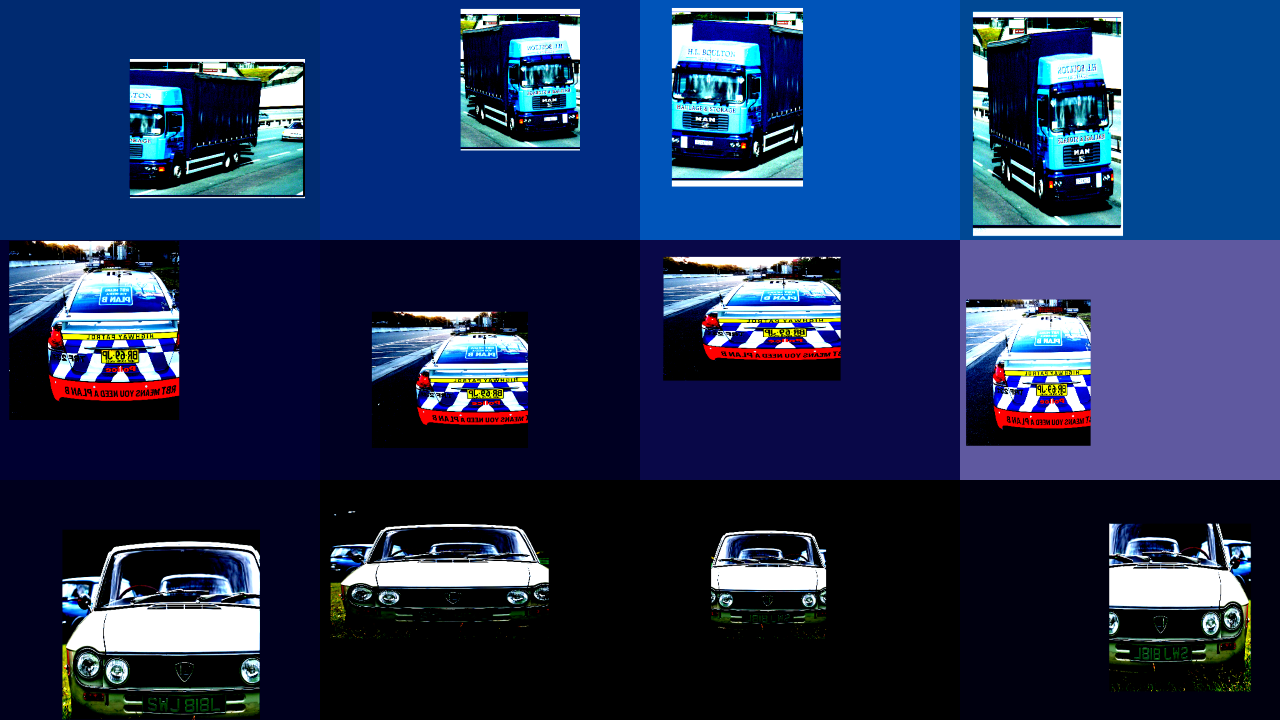
\includegraphics[width=0.8\columnwidth]{.//Figure/PlateLocalization/img_augmentation.png}}
 \caption{Randomly augmented image samples during training. The same transformation is needed for an image and its bounding boxes.}
 \label{fig:img_augmentation}
\end{figure}

\subsection{Optimization}

In this part, I compare the models by summarizing their results in tables. Since multiple values were measured, I only display mAPs. All the trained models' metrics (training duration, mAP, loss) can be viewed in a comprehensive table in the Appendix. For length reasons, I use some abbreviations in the Tables of this section. The metrics \textit{@.50, @.75, small, medium, large} are the mAP values at the corresponding IoU thresholds and object sizes based on the COCO evaluation metrics\cite{MS-COCO}. Model sizes are provided in megabytes. The single numeric value in the input columns is the pixel width and length of the input image. The lr columns stands for learning rate.

Once the input configurations were selected, I started training the models. In the beginning, to save time, I used pre-trained weights (on the COCO 2017 dataset). I kept the same settings of the networks as they were pre-trained. I applied cosine decay learning rate in each case to prevent too optimistic gradient change at the beginning (started from \(\frac{1}{40}\) of the base learning rate, trained like this for \(\frac{1}{20}\) of time, then increased it).

Since training a detector is time-consuming, I drew conclusions based on the results and the learning curve's nature after three epochs (around 17,000 images). One epoch is when the entire dataset is passed forward and backward through the network. The best solution is to apply early stopping (training finishes when model performance permanently stagnates/falls back). However, fewer training sessions would have been possible in this case because there is a minimal improvement over a long period at the end of the flattened learning curve.

I used the same anchor box configuration for all the networks. I used five different-sized grids with a total of 12,804 anchor boxes.

\subsubsection{Architectures}

Generally, a two-stage detector takes a classifier and evaluates it in different locations. Because of the separate steps, these are slower architectures but perform better with various-sized objects. TensorFlow Object Detection API currently supports Faster R-CNN from these variants. Although the inference speed is comparable to one-staged architectures, TFLite conversion is not working – therefore, I solely concentrated on one-stage detectors. SSD, RetinaNet, EfficientDet are supported (YOLO is missing and not likely to be added). Since the detector needs to run on smartphones, choosing a relatively small and fast model was the priority. To start with, I tried 3 different options: RetinaNet (ResNet50), RetinaNet (MobileNetV2), and EfficientDet (EfficientNetD0). I did not try VGG-16 because it is no longer used in modern architectures due to its too many parameters. I used all the networks with the smallest possible input size. Table \ref{tab:starter_architectures} shows the comparison of the starter architectures.

\begin{table}[htb]
\caption{Comparison of the starter architectures.}
\label{tab:starter_architectures}
\noindent
\centering
\begin{tabular*}
{\columnwidth}{@{\extracolsep{\stretch{1}}}*{10}{r}@{}}
    model & size & input & batch & mAP & @.50 & @.75 & small & medium & large\\ \hline
    ResNet50 & 241 & 640 & $8$ & $\textbf{0.389}$ & $\textbf{0.678}$ & $\textbf{0.404}$ & $\textbf{0.116}$ & $\textbf{0.394}$ & $\textbf{0.531}$\\
    EfficientNetD0 & 42 & 512 & $16$ & $0.314$ & $0.581$ & $0.302$ & $0.019$ & $0.321$ & $0.492$\\
    MobileNetV2 & 19 & 320 & $16$ & $0.278$ & $0.504$ & $0.269$ & $0.007$ & $0.248$ & $0.492$\\
\end{tabular*}
\end{table}

I found this comparison problematic as the performance was suspiciously proportional to the input size of the models. It is also important to note that ResNet50 was trained with batch size eight because I had insufficient memory to train it with 16-sized batches. To fix these issues, I switched to EfficientNetD1 and MobileNetV2 640, and the same batch/step values have been applied. Table \ref{tab:starter_architectures_same_input} shows the results.

\begin{table}[htb]
\caption{Comparison of different types with the same input size.}
\label{tab:starter_architectures_same_input}
\noindent
\centering
\begin{tabular*}
{\columnwidth}{@{\extracolsep{\stretch{1}}}*{10}{r}@{}}
    model & size & input & batch & mAP & @.50 & @.75 & small & medium & large\\ \hline
    ResNet50 & 241 & 640 & $8$ & $0.389$ & $\textbf{0.678}$ & $\textbf{0.404}$ & $0.116$ & $0.394$ & $0.531$\\
    EfficientNetD1 & 63 & 640 & $8$ & $\textbf{0.391}$ & $0.671$ & $0.400$ & $\textbf{0.119}$ & $\textbf{0.396}$ & $\textbf{0.548}$\\
    MobileNetV2 & 19 & 640 & $8$ & $0.379$ & $\textbf{0.678}$ & $0.386$ & $0.115$ & $0.386$ & $0.517$\\
\end{tabular*}
\end{table}

This comparison shows more balanced results. Unless ResNet50 is the largest model, its performance is not outstanding anymore; EfficientNet seems to outperform it. MobileNet has modest results; however, it is still close to the benchmark.

As inference speed and model size are critical aspects, ResNet should not be considered. EfficientNet is four times larger than MobileNet: the former runs in 54 ms according to TensorFlow's benchmark, while the latter runs in 39 ms. I measured around 150 ms for EfficientDet and 80 ms for MobileNet on a Samsung Galaxy S10 smartphone running on a CPU with dynamic quantization. Their mAPs are relatively close, so I experimented with both networks before committing to one.

\subsubsection{Batch size}

Batch size is the number of samples propagated through the network at once. Bigger batches allow computational speedups but reduce the ability to generalize. On the other hand, if a model is trained with too small batch sizes (perhaps caused by too sample-specific gradient updates), performance decreases. An ideal range of batch sizes is affected by model parameters and the current dataset.

I trained both networks with different batch sizes. The maximum size I could use was 8 in the case of EfficientNet and 24 for MobileNet. When training with batch size 1, I reduced the learning rate by an order of magnitude (from \({8} \times {10^{-2}}\) to \({8} \times {10^{-3}}\)) to avoid divergence caused by too large gradient updates. Results can be observed in Table \ref{tab:different_batch_sizes}.

\begin{table}[htb]
\caption{Training results with different batch sizes.}
\label{tab:different_batch_sizes}
\noindent
\centering
\begin{tabular*}
{\columnwidth}{@{\extracolsep{\stretch{1}}}*{10}{r}@{}}
    model & size & input & batch & mAP & @.50 & @.75 & small & medium & large\\ \hline
    MobileNetV2 & 19 & 640 & $24$ & $0.386$ & $0.669$ & $0.376$ & $0.108$ & $0.367$ & $0.512$\\
    MobileNetV2 & 19 & 640 & $16$ & $0.372$ & $0.666$ & $0.378$ & $0.101$ & $0.381$ & $0.508$\\
    MobileNetV2 & 19 & 640 & $8$ & $0.379$ & $0.678$ & $0.386$ & $0.115$ & $0.386$ & $0.517$\\
    MobileNetV2 & 19 & 640 & $4$ & $0.377$ & $0.677$ & $0.381$ & $0.116$ & $0.385$ & $0.507$\\
    MobileNetV2 & 19 & 640 & $1$ & $0.261$ & $0.535$ & $0.225$ & $0.090$ & $0.327$ & $0.301$\\
    EfficientNetD1 & 63 & 640 & $8$ & $\textbf{0.391}$ & $0.671$ & $\textbf{0.400}$ & $\textbf{0.119}$ & $0.396$ & $\textbf{0.548}$\\
    EfficientNetD1 & 63 & 640 & $4$ & $0.388$ & $\textbf{0.681}$ & $0.390$ & $\textbf{0.119}$ & $\textbf{0.398}$ & $0.541$\\
    EfficientNetD1 & 63 & 640 & $1$ & $0.291$ & $0.578$ & $0.262$ & $0.100$ & $0.330$ & $0.373$\\
\end{tabular*}
\end{table}

Based on the results, batch sizes 4 and 8 were the most optimal. Both networks produced the most accurate outputs trained with batch size 8. At larger sizes, a decline is observed, especially in detecting small objects. Regarding the other extreme at batch size 1, gradient update per every image seems to confuse the network and reduce its performance. The trend is MobileNet lags by 2-3\% mAP in every configuration behind EfficientNet. On the other hand, MobileNet is four times smaller and significantly faster but slightly less accurate. For these reasons, I decided to use MobileNetV2 for the rest with batch size 8.

\subsubsection{Optimization algorithm and learning rate}

Optimization algorithms\cite{overviewSGD} are used to update network parameters (such as weights) to minimize model loss while training. The most popular method is Stochastic Gradient Descent and its mini-batch variant. This algorithm is relatively easy and powerful, but it usually results in slow convergence. Momentum optimization is generally applied to overcome this issue, introducing and updating gradients' velocity instead of their specific value. Different optimizers exist, such as methods using an adaptive learning rate like RMSprop or Adam.

I tried the Adam, Momentum, and the RMSprop algorithms. Initially, I used the same learning rate \(({8} \times {10^{-2}})\) in all three cases. However, training indicators in the case of Adam and RMSprop showed signs of divergence, so I changed their values to their default learning rate \(({2} \times {10^{-3}})\) based on TensorFlow's optimizer definition. It seems that Momentum's recommended optimum is roughly an order of magnitude larger than what is ideal for the other two. Table \ref{tab:different_opt_algorithms} shows the results.

\begin{table}[htb]
\caption{Comparison of the different optimization algorithms. All the models are MobileNetV2 variants.}
\label{tab:different_opt_algorithms}
\noindent
\centering
\begin{tabular*}
{\columnwidth}{@{\extracolsep{\stretch{1}}}*{9}{r}@{}}
    input & lr & optimizer & mAP & @.50 & @.75 & small & medium & large\\ \hline
    640 & $0.002$ & $Adam$ & $\textbf{0.392}$ & $\textbf{0.682}$ & $\textbf{0.410}$ & $0.103$ & $\textbf{0.412}$ & $0.546$\\
    640 & $0.08$ & $Momentum$ & $0.391$ & $0.671$ & $0.400$ & $\textbf{0.119}$ & $0.396$ & $\textbf{0.548}$\\
    640 & $0.002$ & $RMSprop$ & $0.361$ & $0.643$ & $0.374$ & $0.079$ & $0.394$ & $0.512$\\
    640 & $0.08$ & $RMSprop$ & $0.155$ & $0.333$ & $0.130$ & $0.007$ & $0.154$ & $0.213$\\
    640 & $0.08$ & $Adam$ & $0.011$ & $0.031$ & $0.004$ & $0.000$ & $0.000$ & $0.018$\\
\end{tabular*}
\end{table}

The last two rows of Table \ref{tab:different_opt_algorithms} show the typical cases of too high learning rates. With values closer to their optimums, algorithms could be compared more realistically. Adam and Momentum produced very similar results, while RMSprop could not perform at their level. However, before concluding, the nature of the learning curves is also worth analyzing to see which algorithm has started to converge and which is still improving.

\begin{figure}[htb]
 \centerline{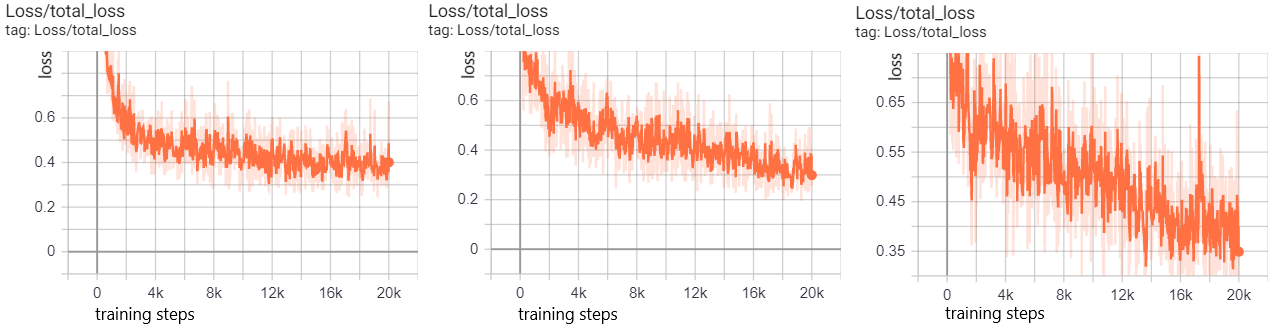
\includegraphics[width=1.0\columnwidth]{.//Figure/PlateLocalization/optimization_algorithm_comparison.png}}
 \caption{Total loss trends of RMSprop (left), Momentum (center), and Adam (right).}
 \label{fig:optimization_algorithm_comparison}
\end{figure}

Figure \ref{fig:optimization_algorithm_comparison} shows that RMSprop not only lags behind but already converges strongly and slightly improves after 14,000 steps. On the other hand, Momentum and Adam still improve. Out of the two, Adam oscillates more, which may sign a too high learning rate. However, the constant improvement after 20,000 steps (and the fact that I use decay learning rate, but oscillation does not decrease) instead suggests that this is more of behavior due to the algorithm's nature, which needs further investigation. Another thing to spot: although Adam performs better in almost everything, Momentum has a significant edge in training detectors to find small objects.

Therefore, I executed another 20,000 steps with the last two algorithms, and I also tried Adam with an order of magnitude lower learning rate \(({2} \times {10^{-4}})\). After this iteration, each case surpassed the optimum and started to overfit. Table \ref{tab:best_optimization_algorithms_comparison} shows the results. It seems that Momentum has the edge: it has improved until reaching 0.393 mAP, while the best of Adam is 0.391, before stagnating around 0.387. The latter could not improve with the lower learning rate, resulting in 0.383 mAP. Thus, the final model to take is the one trained with Momentum.

\begin{table}[htb]
\caption{Comparison of the best results of Momentum and Adam. All three cases indicate the best-performing models before overfitting. All the models are MobileNetV2 variants.}
\label{tab:best_optimization_algorithms_comparison}
\noindent
\centering
\begin{tabular*}
{\columnwidth}{@{\extracolsep{\stretch{1}}}*{10}{r}@{}}
    input & lr & optimizer & mAP & @.50 & @.75 & small & medium & large\\ \hline
    640 & $0.008$ & $Momentum$ & $\textbf{0.393}$ & $\textbf{0.686}$ & $0.391$ & $\textbf{0.119}$ & $0.392$ & $\textbf{0.545}$\\
    640 & $0.002$ & $Adam$ & $0.391$ & $0.685$ & $\textbf{0.404}$ & $0.108$ & $\textbf{0.404}$ & $0.543$\\
    640 & $0.0002$ & $Adam$ & $0.383$ & $0.669$ & $0.380$ & $0.116$ & $0.390$ & $0.528$\\
\end{tabular*}
\end{table}

\subsection{Model deployment}

When the model training is ready, it is time for quantization, TFLite conversion, and to generate the auxiliary structures for deployment.

\subsubsection{TensorFlow Lite conversion and quantization}

During model conversion, it is necessary to note that not all TensorFlow operations are implemented in TFLite. To avoid conversion problems, I checked the compatibility table to see whether the operations in the model (e.g., activation function, depthwise convolution) could be converted. The resulting TensorFlow Lite file at the end of the process can run on Android devices using an interpreter.

\begin{figure}[H]
 \centerline{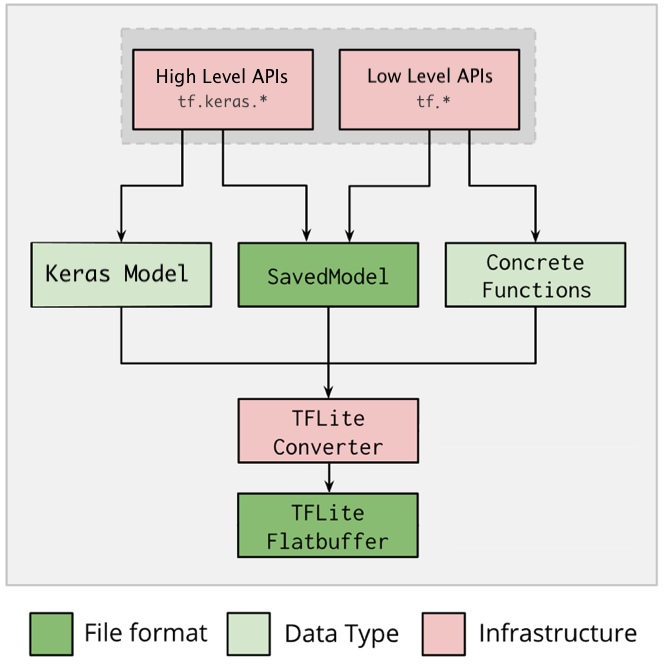
\includegraphics[width=0.5\columnwidth]{.//Figure/PlateLocalization/tflite_converter.png}}
 \caption{TensorFlow Lite conversion process. Source: \cite{TensorFlowLiteConverter}}
 \label{fig:tflite_converter}
\end{figure}

\subsubsection{Input- and output formats}

The detector expects $640\times640$ pixel RGB images on its input. The input is channels\char`_last encoded (order of indices: height, width, red, green, blue). The value of one channel of a pixel is encoded in 8 bits (1 byte). On all three RGB channels, the values are interpreted as 8-bit integer numbers, which must be between 0 and 255.

The model outputs a Hash Map containing four arrays mapped to the indices 0-3. Arrays 0, 1, and 2 describe 100 detected objects, with one element in each array corresponding to each object. There are always 100 detection proposals. A brief description of the arrays is as follows:

\begin{itemize}
  \item \textit{Boxes}: Multidimensional float32 tensor of shape [1, num\char`_boxes, 4] with box locations. Floating-point values are between 0 and 1, the inner arrays representing bounding boxes in the form [top, left, bottom, right].
  \item \textit{Classes}: A float32 tensor of shape [1, num\char`_boxes] with class indices, each indicating the index of a class label from the labels file.
  \item \textit{Scores}: A float32 tensor of shape [1, num\char`_boxes] with class scores. Values between 0 and 1 represent the probability of the detected class.
  \item \textit{Number of boxes}: float32 tensor of size 1 containing the number of detected boxes.
\end{itemize}

\subsubsection{Auxiliary structures}

It is necessary to use an auxiliary structure to interpret the output of the detector. To do this, I created a file containing the names of the output classes in the correct order line by line, including the background class.

The file model\char`_info.txt explains the corresponding model. It contains general information about the network, such as the definition and interpretation of the input and output data formats required for use.

\subsubsection{Summary}

This section dealt with data preparation, architecture selection, training and fine-tuning, and the detector post-production steps. I concluded a total of 184 hours of training with 23 different configurations. The detailed results of the final model can be seen in the table below. Compared to the first initial training from this network family, 1.4\% gain has been reached in COCO mAP. The final detector's size is 35.38 MB, its quantized counterpart is 11.19 MB. Some properties of the selected model are shown in Table \ref{tab:final_model_summary}.

\begin{table}[htb]
\caption{Final model training properties. The architecture is MobileNetV2 trained with the Momentum optimizer (learning rate=\({2} \times {10^{-4}}\), batch size 8).}
\label{tab:final_model_summary}
\noindent
\centering
\small\begin{tabular*}
{\columnwidth}{@{\extracolsep{\stretch{1}}}*{11}{r}@{}}
    input & steps& pre-trained? & duration & mAP & @.50 & @.75 & small & medium & large\\ \hline
    640 & $30,000$ & Yes (COCO) & 8h 50m & $0.393$ & $0.686$ & $0.391$ & $0.119$ & $0.392$ & $0.545$\\
\end{tabular*}
\end{table}
%----------------------------------------------------------------------------
\chapter{Optical character recognition}

This chapter focuses on the OCR (Optical character recognition) part of the ALPR process. I propose a lightweight algorithm that is part of a vehicle identification pipeline capable of running on Android smartphones.

Optical character recognition consists of character localization- and classification. It is responsible for producing machine-encoded text from a text image. First, character segmentation is applied, separating individual characters on the image. The name is a bit misleading as it can be object detection or semantic segmentation. Then follows classification, which is about outputting one machine-encoded character based on an image of a single character.

There are two main approaches regarding Optical Character Recognition with deep learning. Object detection can be used to locate individual characters on images. This solution outputs a character score for each detected box, instantly recognizing tokens in multiline plates. However, there are significant drawbacks in the context of OCR\cite{CTCexp}:

\begin{itemize}
  \item Annotating real-life datasets on a character level is time-consuming.
  \item Detectors usually struggle with small objects (like characters in text).
  \item The outputs are character scores, and therefore further pre-processing is needed to get the final text from it.
  \item When using fixed boxes, a single character can trigger multiple positions. It is possible that ``GGOO'' is the prediction because the ``O'' is wide. In that case, we must remove all duplicate tokens. Nevertheless, it can be that the original text would have been ``GGO''. Then removing the duplicates produces a wrong result.
\end{itemize}

Another approach can be the sequential feature extraction with convolutional and recurrent layers guided by Connectionist Temporal Classification\cite{CTC}. In this solution, the convolutional part extracts the necessary features. Then the recurrent part processes them sequentially to output a probability for each time step. The main advantage over the object detection approach is that only an image and the target text need to be provided; CTC handles the rest. Therefore, character positions and width are ignored, which makes it easier to label real-life datasets. An output sequence of a CRNN can be easily translated into a text with either the Greedy or Beam search algorithms, as CTC also indicates the end of the characters with a specific token. However, these solutions can process images along one axis (practically horizontally); therefore, they cannot recognize multiline blocks in standalone versions.

Different approaches exist to convert CRNNs into multiline recognizers. The classical solution can be the Scale Space Technique for Word Segmentation\cite{ScaleWordSeg}, which outputs block positions. It performs relatively well (87\%) on handwritten papers. For multiple text block recognition, both an object detector or an image segmentation model can be used first, and their outputs then fed into the CRNN. However, this solution is wasteful as an image must be processed multiple times, and low-level feature extractions are not shared across individual networks. Recently, Wojna et al.\cite{Attention-basedExtract} proposed an end-to-end model with an attention mechanism. OrigamiNet\cite{OrigamiNet} introduced a one-step model by learning to unfold, transforming existing CRNNs into multiline recognizers. Other approaches still exist, like proposed by WPOD-NET\cite{WPOD-NET}, where a modified YOLO detector is used for OCR purposes.

\section{Data}

An adequate amount of data is required to train a deep learning algorithm. There were only a few number plate datasets for object detection (which were missing text labels). The OCR sets neither satisfied the search as they were too specific in domains like handwriting recognition or housing numbers. A good option where there are 15 million annotated images is the database of platesmania.com\cite{PlatesMania}. However, their API access proved to be expensive even for chunks of 50,000 images, as is their offline license plate generator script.

The nature of license plates varies between countries or even provinces. There are plenty of structures, colors, and fonts (like the modified Mittelschrift in Hungary or the Mandator font in the UK). There can be single-line vs. multi-line versions. Some countries use non-Latin alphabets (like China or Egypt), which makes the task even harder. Figure \ref{fig:plates} shows some example license plates. Taking these into account, I aim to recognize Latin alphabet characters; 17 currently used number plate fonts have been collected from Australia, North America, and Europe.

\begin{figure}[htb]
 \centerline{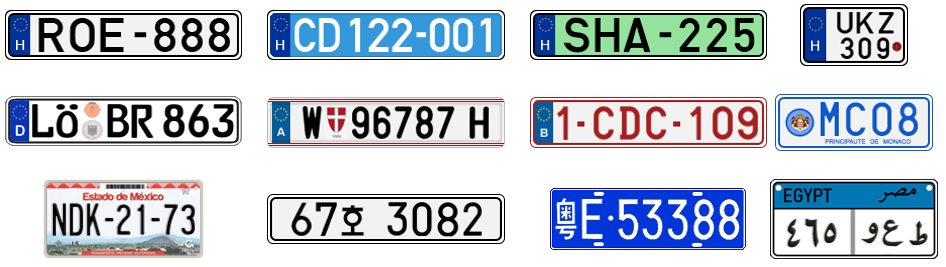
\includegraphics[width=1.0\columnwidth]{.//Figure/OCR/plates.png}}
 \caption{License plates from Hungary (1st row), Europe (2nd row), and other continents (3rd row).}
 \label{fig:plates}
\end{figure}

A few characters are traditionally hard to distinguish in the Latin alphabet, like 0-O-Q, 1-I, or 8-B. This issue is often eliminated by prohibiting letters and numbers on the same character position. However, as plate structures can vary even in a single country, this is not a general solution. Moreover, two different characters may be the same in a font (like 0-O in the Mandatory) or across different fonts. Therefore, I decided that the unique items to distinguish are 0-9 and A-Z excluding O, plus the hyphen (10 + 25 + 1 characters). Other difficulties arise from picture quality and visibility aspects (lighting, contrast, rotation, motion-blur). This diversity suggests a general OCR model has the edge over systems based on hand-crafted feature extraction for each plate type.

For this reason, I implemented a data generator, which approaches the task at the character level. It uses three types of resources to create an output: a list of characters to generate random text, fonts, and overlay images to mimic dirt, ice, and other phenomena. The generator also handles character-level bounding boxes to be converted to output detector training data, producing multiple text blocks. Creating one $200\times200$ RGB image takes roughly 30 ms without bounding boxes and 61 ms with them. The generator applies data augmentation techniques to enrich data diversity. Algorithm \ref{alg:data_generator_pipeline} shows the individual steps of the pipeline.

\begin{algorithm}
\caption{Data generator pipeline}
\label{alg:data_generator_pipeline}
\begin{algorithmic}[1]
 \STATE \textbf{procedure} Generate($args$)
 \STATE random font and image overlay from $args$
 \STATE $bckgColor$ = random value [0...255] in every channel
 \STATE $image$: create with defined dimensions from $args$ and $bckgColor$
 \STATE $generatedTexts$ = $args[numBlocks]$ random texts in the range of 1...10.
 \STATE $lastBoxCoords$ = [0,0,0,0]
 \STATE $insertedTextIndices$ = []
 \FOR{$text$ in $generatedTexts$}
 \STATE $textColor$ = text and background colors must have at least 20\% diff in one channel (randomly selected which channel satisfy this)
 \STATE $textImage$: create text image from $text$, with a background color identical to $bckgColor$
 \IF{$textImage$ is bigger than $image$ in any dimension}
 \STATE $textImage$: resize to fit onto the $image$
 \ENDIF
 \STATE $textImage$: resize ratio with a value in the resize range (typically 0.85...1)
 \STATE $textImage$: random aspect ratio change, heigh, and width offset
 \IF{($lastBoxCoords[3]$ < $boxYstart$) || (($lastBoxCoords[2]$ < $boxXstart$) \&\& ($lastBoxCoords[1]$ < $boxYstart$))}
 \STATE $image$ += $textImage$
 \STATE $lastBoxCoords$ = [$boxXstart$, $boxYstart$, $boxXend$, $boxYend$]
 \STATE $insertedTextIndices$ += currentBoxIndex
 \ENDIF
 \ENDFOR
 \STATE $image$: random rotation and perspective transformation
 \STATE $image$: resize to the required size
 \STATE $image$ += random overlay with offset and rotation
 \STATE $image$: random brightness, contrast, sharpness, gaussian blur (within $args$ constraints)
 \STATE $image$: downscale between a range from $args$, then scale back
 \STATE $image$: normalize from [0...255] to [-1...1), convert to float32
 \STATE $label$ += $text$ which Id is in $insertedTextIndices$
 \STATE $label$: encode $label$ to a number label with dictionary from $args$
 \STATE return $image$, $label$
\end{algorithmic}
\end{algorithm}

As the validation samples are also generated, the images must be equally distributed across different evaluation sets. A single evaluation epoch is set to contain 10,000 images. With this size, there is a maximum of +/-0.015 deviation in loss across multiple validations. Figure \ref{fig:generated} shows some random one-line generated sample.

\begin{figure}[htb]
 \centerline{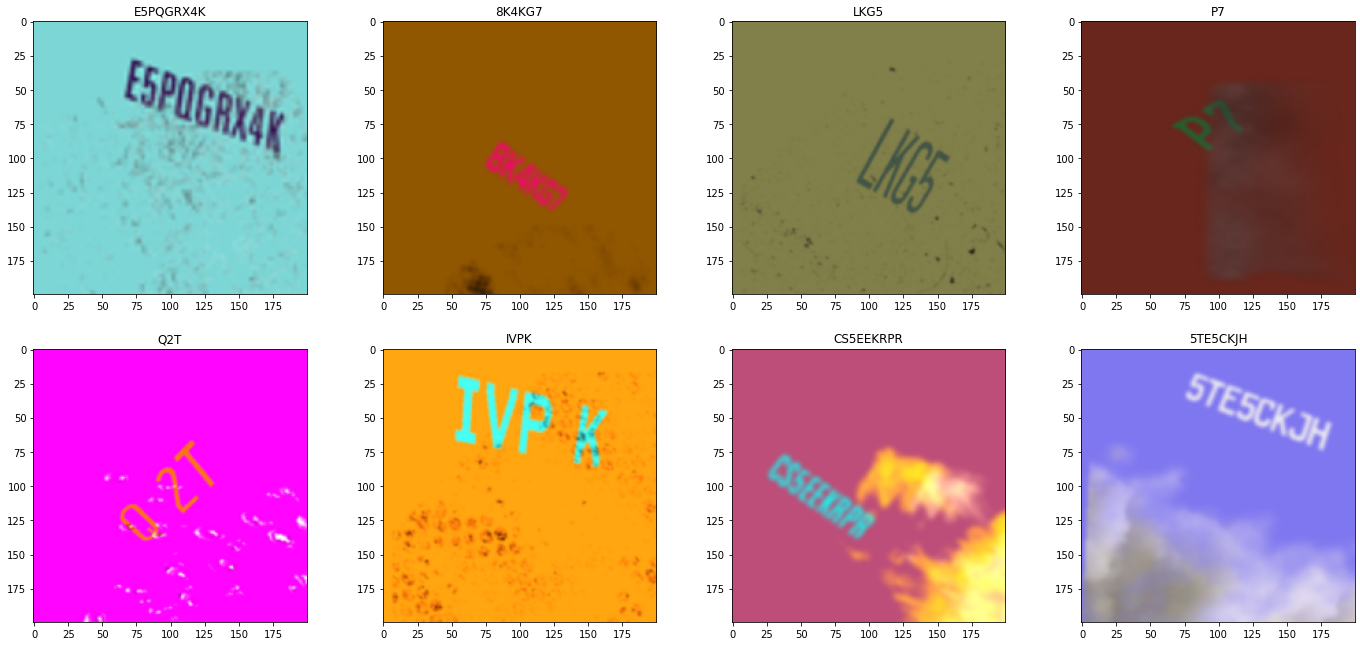
\includegraphics[width=1.0\columnwidth]{.//Figure/OCR/generated.png}}
 \caption{One line generated samples with labels on top. Hard overlays have been removed from the validation set so that the completely illegible characters do not affect results.}
 \label{fig:generated}
\end{figure}

\section{Sequential approach}

My first OCR approach is based on feed-forward recurrent convolutional networks (CRNN) that produce fixed-size arrays of character probabilities.

\subsection{Connectionist Temporal Classification}

Connectionist Temporal Classification\cite{CTC} is used to compute model loss. The cost function has a barely documented Keras implementation, which I wrapped into a layer to make it easily detachable after training. This layer has two inputs: model prediction (\textit{batch\_size, max\_timesteps, num\_characters}) and ground truth encoded as numbers (\textit{batch\_size, max\_len}). Besides the 36 identifiable items, two more numbers are indicating the non-character token and the unknown character. Inputs must be the same length in a single batch. If a label's text is shorter than the maximum length, padding is expected with non-character tokens. The padding ensures that the model can be trained with greater batches than one, as multiple labels can be merged into a single, same dimensional array. The layer deduces the length of each label at runtime before computing its cost. To do that with arbitrary batches, I had to put a loop into the layer. The implemented TensorFlow loop is 30\% slower than the Python counterpart, but it can be placed on a TensorFlow graph.

\subsection{Building blocks}

A custom convolution layer is defined with Convolution $\rightarrow$ Nonlinearity $\rightarrow$ Dropout $\rightarrow$ Batch Normalization (Figure \ref{fig:blocks}). These types of layers are stacked on top of each other in the residual blocks. The implementation allows to specify the type of activation function, the proportion of dropout, and whether to use Batch Normalization or not (when enabled, it adds bias to the output, so the convolution operation's bias is disabled in that case). Every convolution operation uses ``SAME'' padding. It applies padding so that the whole input gets fully covered by the filter and specified stride. The name comes from that, for stride 1, the size of the output is the same as the input. This partly solves the skewed kernels and feature-map artifacts issue induced by the operation\cite{PadBlindSpot}.

The main parts of the network are the residual blocks which consist of three components. The residual stage contains an arbitrary number of convolution layers with the same input/output size and channels. This block of layers is defined with a skip connection between the input and the output to overcome the vanishing gradient problem, which that means the block's input directly influences its output through a ``gradient highway'', not just through convolutions. After that, an upscaling convolution layer doubles the number of channels (it is the only layer that gradients cannot bypass; therefore, it is a bottleneck). It is followed by spatial downscaling by a factor of two with pooling. The structure is illustrated by Figure \ref{fig:blocks}. In this configuration, a block with input dimensions (height, width, channels) has an output of \((\frac{height}{2}, \frac{width}{2}, channels\times2)\). My implementation was inspired by the ResNet\cite{ResNet} architecture.

\begin{figure}[htb]
 \centerline{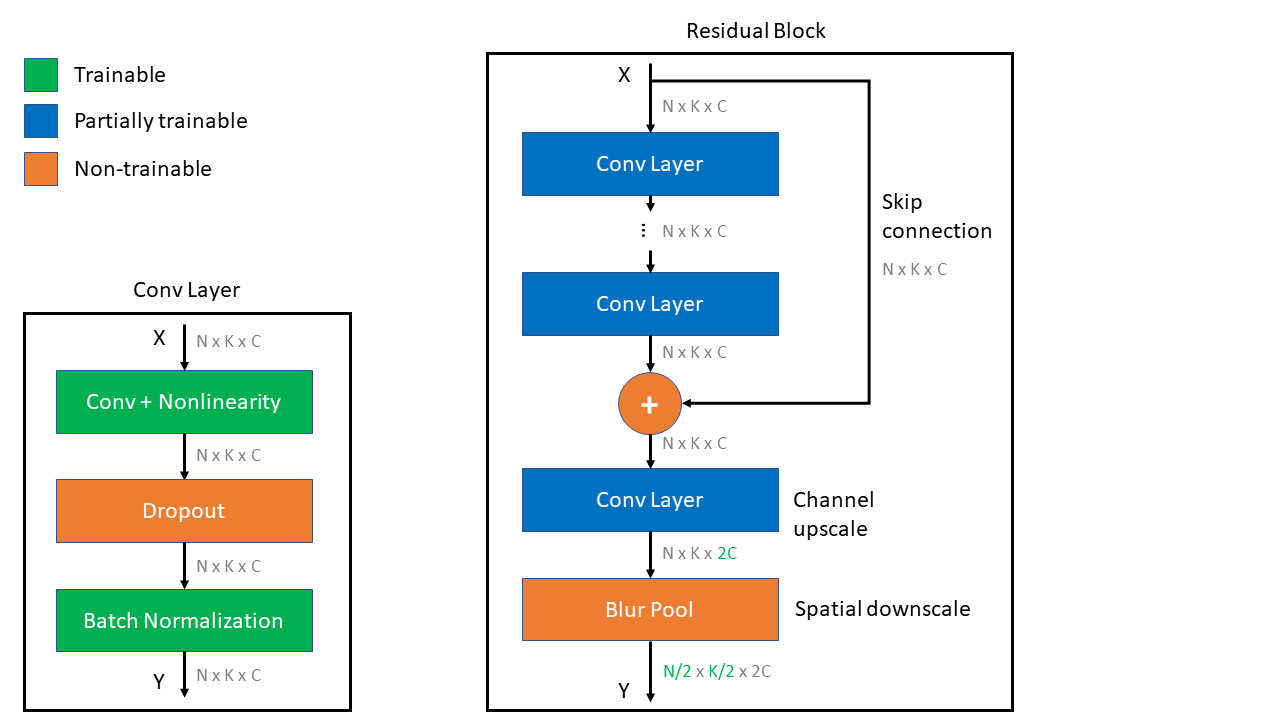
\includegraphics[width=1.0\columnwidth]{.//Figure/OCR/blocks.png}}
 \caption{Network building blocks with the convolution layer (left) and the residual block (right).}
 \label{fig:blocks}
\end{figure}

In the recurrent part of the network, two Long Short-Term Memory\cite{LSTM} layers are stacked on top of each other responsible for sequential processing. At the time of this work, GRU TensorFlow Lite support was unavailable, so I could only use LSTM for smartphone inference. In the network's first layer, the height and width dimensions of the input are swapped so that the width is the first dimension in the model. Thus, recurrent layers process inputs horizontally. A dense layer follows the last LSTM layer with a dimension of (${input\_width}\times{downscale\_factor}$, \textit{num\_characters}), which is the network's output matrix. The high-level operation of the model is illustrated in Figure \ref{fig:processing_steps}.

\begin{figure}[htb]
 \centerline{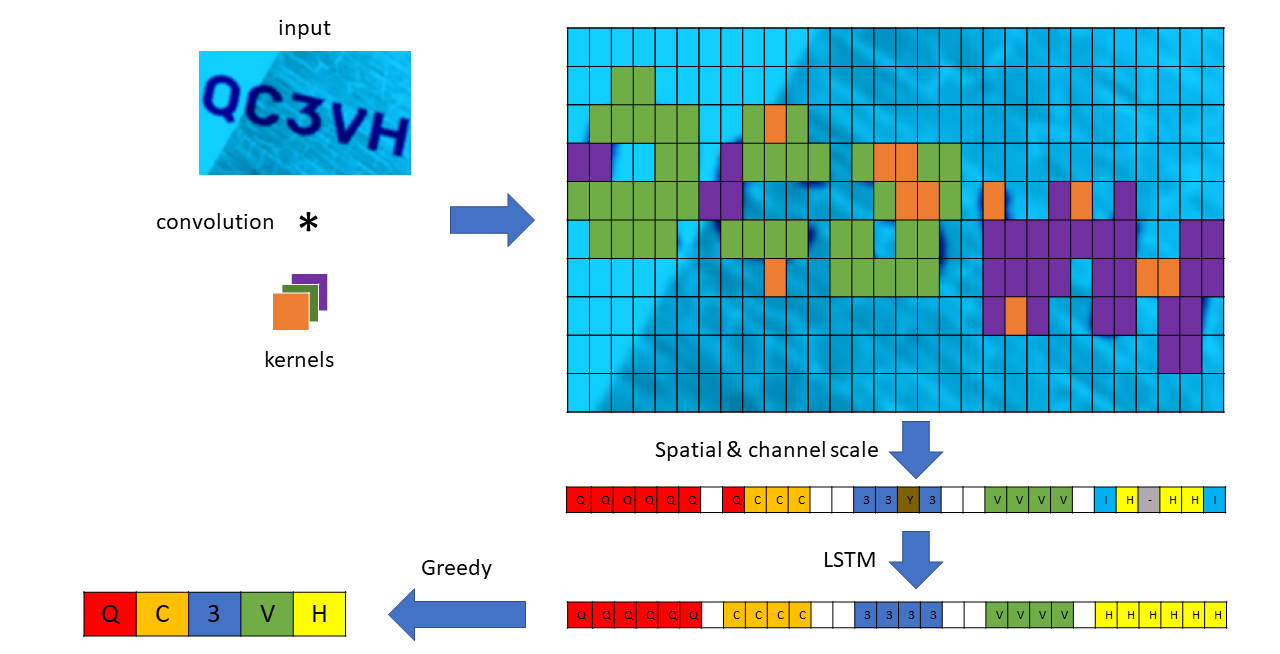
\includegraphics[width=1.0\columnwidth]{.//Figure/OCR/processing_steps.png}}
 \caption{Simplified representation of the network's key processing steps.}
 \label{fig:processing_steps}
\end{figure}

The best model has a downscale factor of three (number of residual blocks) and an input image width of 500 pixels, which means 63 steps overall. One window has a width of 8 pixels. Each window must be assigned to a real or an empty character token. It means that net 31 characters can be recognized to have enough space for characters and empty tokens in the output matrix.

\subsection{Greedy search}

In training, the CTC layer handles raw model outputs and ground truth labels, then calculates loss to backpropagate. However, this is not required for inference. Multiple approaches are available to decode raw outputs of the last dense layer. The Greedy solution keeps the maximum index at each step, then merges the same tokens between empty tokens. This way, multiple recognitions triggered by the same character are eliminated. The next step is to remove the empty tokens and decode the sequence with the model's vocabulary. That step produces the final text. Other approaches, like Beam search, iteratively create text candidates, arranges them based on their probability scores, and keeps the best ones after every iteration. The most probable beam at the end is returned as a result. This algorithm can be highly computation-intensive depending on the number of beams. Word Beam Search\cite{WordBeamSearch} takes this idea to another level: it constrains beams with a prefix tree of existing words. This solution can be helpful in situations where the words to recognize are from a specific vocabulary, but in the case of plate recognition, such a semantic assumption does not help. For these reasons, I implemented the Greedy algorithm.

\subsection{Experiments}

As a starting point, the model is trained with two residual blocks with a single convolution layer in each. The first block starts with 32 input channels, and the batch size is 8. Adam optimizer\cite{Adam} is used with the default parameters (\({1} \times {10^{-3}}\) learning rate). One epoch is equal to 100,000 images, and early stopping is applied with five epoch patience. This model reached the optimum after 13 epochs with a validation loss of 0.2298. I tried different batch sizes to find the most optimal as shown in Table \ref{tab:batch_sizes}.

\begin{table}[htb]
\caption{The effect of batch sizes. Smaller batches converged faster at the beginning of training, but their improvement flattened out earlier at worse sub-optimal points. Batch size 128 was the largest that could fit into the memory.}
\label{tab:batch_sizes}
\noindent
\centering
\begin{tabular*}
{\columnwidth}{@{\extracolsep{\stretch{1}}}*{3}{r}@{}}
    batch & epochs & loss\\ \hline
    8 & $8$ & $0.2121$ \\
    16 & $29$ & $0.1545$ \\
    32 & $22$ & $0.1134$ \\
    64 & $55$ & $0.0855$ \\
    128 & $51$ & $\textbf{0.0848}$ \\                   
\end{tabular*}
\end{table}

\subsubsection{Shift-invariance}

Zhang et al.\cite{Shift-Invariant} pointed out that modern CNNs lack shift-invariance since max-pooling, average-pooling, and strided-convolution ignore Nyquist's sampling theorem. The proposed solution is the use of blur-pooling, where spatial downsampling happens (Figure \ref{fig:anti_aliasing}). I implemented blur-pooling with separable kernels and replaced all the other pooling layers with them. Although they claim that the solution is compatible with the layers listed above, I wanted to keep the number of layers as low as possible. The shift-invariant model slightly improved in loss, but a lot in the speed of convergence. Therefore, I continued to work with this model as the new benchmark.

\begin{figure}[htb]
 \centerline{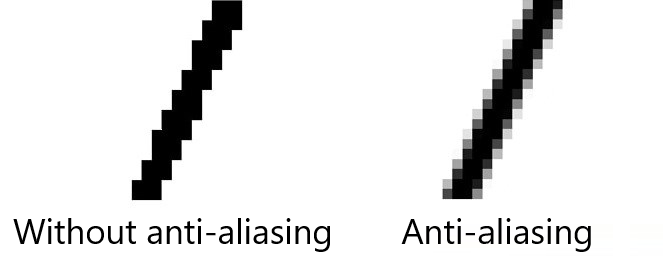
\includegraphics[width=0.6\columnwidth]{.//Figure/OCR/anti_aliasing.png}}
 \caption{The effect of anti-aliasing when scaling down a sloped line. Blur-pooling prevents the appearance of too sharp artifacts.}
 \label{fig:anti_aliasing}
\end{figure}

\subsubsection{1D convolution}

I experimented with using 1D convolutional layers instead of the LSTM cells. This way, the model does not have any recurrent part, only residual blocks with convolutions. The more straightforward structure without loops results in faster runtimes. However, the training became significantly longer, and the final result lagged behind the benchmark (0.08 vs. 0.1). The primary source of error was that one character triggered multiple different classifications based on the sequential processing's actual position. While LSTM can effectively smooth out 1D feature maps (``OCOO'' $\rightarrow$ ``OOOO''), it looked like 1D convolution had a more challenging time. Therefore, I no longer used this approach.

\subsubsection{Hyperband optimization}

Hyperparameter optimization has been realized with the Hyperband algorithm\cite{Hyperband}. Another option considered was Bayesian optimization. I chose the former because adaptive Bayesian methods do not handle discrete, independent, unordered values well, and training would have lasted longer (since one configuration is done when the model training stops). Hyperband is a fast guided random search that works like a knockout sports competition: it generates combinations and trains them for a few epochs. After that, the top-performing part of the models is trained further, while the others are discarded. The iteration repeats until all the remaining models stop learning or there is a clear winner. 

Hyperband strongly filters models based on early training performances. Therefore, variable batch size or learning rate was not possible with this algorithm because smaller batches tend to outperform larger ones initially, but not in the long run. The selected parameters to optimize were the number of features of the first block (which is then doubled by every consequent block), kernel size, whether residual connections and batch norm layers are needed, dropout rate, number of blocks, convolutional layers in blocks, and type of activation function. A batch size of 32 was applied during training with every model, as instances with more blocks and layers should also fit into memory. Therefore, the previous batch 32 model served as a baseline. The best configurations found by the optimization algorithm are shown in Table \ref{tab:top3}. Sample inference results can be seen in Figure \ref{fig:inference_sequential}.

\begin{table}[htb]
\caption{Top 3 configurations found by Hyperband. Only the top 2 and the baseline were trained until convergence (3rd model training has been stopped earlier). Columns: model, features, kernel, residual, batch norm, dropout, blocks, layer per block, activation, epochs, loss.}
\label{tab:top3}
\noindent
\centering
\begin{tabular*}
{\columnwidth}{@{\extracolsep{\stretch{1}}}*{11}{r}@{}}
    model & feat & ker & res & bn & drop & b & l & act & epochs & loss\\ \hline
    1st & $64$ & $3$ & $\checkmark$ & $\checkmark$ & $0.09$ & $3$ & $3$ & ReLU & $39$ & $\textbf{0.0753}$ \\
    2nd & $64$ & $5$ & $X$ & $\checkmark$ & $0.2$ & $2$ & $2$ & ReLU & $35$ & $0.0862$ \\
    3rd & $64$ & $3$ & $X$ & $\checkmark$ & $0.3$ & $2$ & $3$ & ELU & $15$ & $0.1554$ \\
    baseline & $32$ & $3$ & $\checkmark$ & $\checkmark$ & $0.1$ & $2$ & $1$ & ReLU & $22$ & $0.1134$ \\           
\end{tabular*}
\end{table}

\begin{figure}[htb]
 \centerline{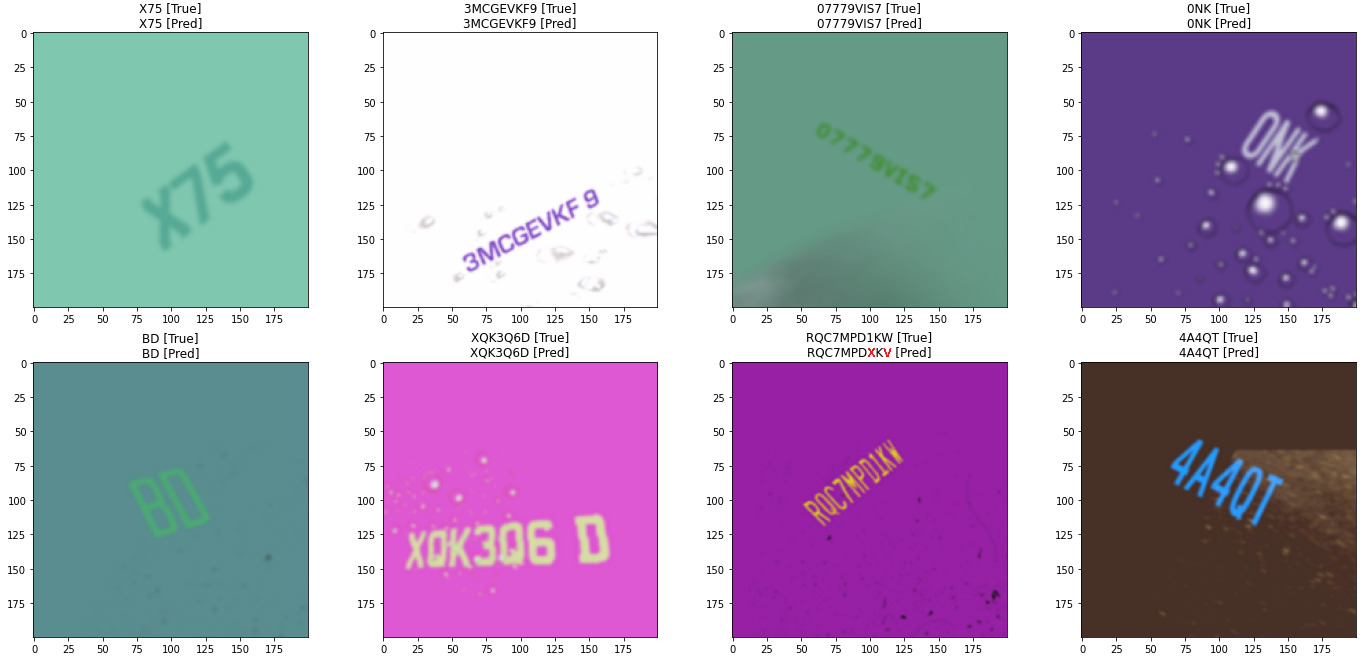
\includegraphics[width=1.0\columnwidth]{.//Figure/OCR/inference_sequential.png}}
 \caption{Inference results of the best performing network. Incorrect characters are marked as red.}
 \label{fig:inference_sequential}
\end{figure}

\subsection{Multiline recognition}

There are numerous approaches to process number plates with multiple lines. One can be the usage of object detection to detect individual text blocks on an image. One powerful model based on this approach is the CRAFT\cite{CRAFT} text detector. Another approach is text segmentation, which is not necessarily done by neural networks. In both cases, however, the recognition of text blocks and characters are separated steps and the weights used for them are not shared. I experimented with a model that merges these steps. The key idea is to add some layers to the end of the network that learns to unfold the two-dimensional feature map into a tall, one-dimensional feature sequence. This approach changes the main axis (the horizontal reading of text changes to process vertical features). To accomplish this, I implemented a modified Origami\cite{OrigamiNet} module that includes convolution layers and resizing with bilinear interpolation. The pseudo code of the module is shown by Algorithm \ref{alg:unfolding}.

 \begin{algorithm}
 \caption{Pseudo code of the Unfolding module.}
 \label{alg:unfolding}
 \begin{algorithmic}[1]
    \STATE \textbf{procedure} Unfolding($inDim, inChannel, outChannel, numBlocks, numLayers$)
    \STATE vertical = inputDim[0]
    \STATE horizontal = inputDim[1]
    \FOR{$i = 0$; $i$ $<=$ $numBlocks$; $i$++}
    \STATE vertical *= 2
    \STATE horizontal /= 2
    \STATE Resizing(vertical, horizontal, interpolation=bilinear)
    \FOR{$j = 0$; $j$ $<=$ $numLayers$; $j$++}
    \STATE Conv(inChannel, inChannel)
    \ENDFOR
    \ENDFOR
    \STATE Conv(inChannel, outChannel, (1, 1), (1, 1))
    \STATE xDownFactor = pow(2, $numBlocks$)
    \STATE xRemain = inDim[1] \% xDownFactor > 0
    \STATE xLastKernelSize = (inDim[0] // xDownFactor) + xRemain
    \STATE Conv(outChannel, outChannel, (1, xLastKernelSize), (1, xLastKernelSize))
\end{algorithmic}
\end{algorithm}

The original solution was not ideal for this task. I had to remove the recurrent part of the original network (LSTM layers) because they introduced instability while training. I replaced pooling with strided convolution, increased the number of resizing steps, reduced the spatial rescaling ratio, and increased the number of convolution layers. After these modifications, the module started working as intended. The best loss was 0.9517 on images with a maximum of five rows of texts after 73 epochs (0.0991 on single line images). It is far from an optimal solution, but all I had to do is to add a module to the end of an existing model. Unfolding also scales well, as the runtime does not change even when processing multi-row text images.

However, unfolding has its drawbacks. The original model had a size of 640 KB, while this module increased it to 3.138 MB. Multiplying the size of a model already reading single-line texts five times seems wasteful (even so, it is less than using a separate detector and a single line recognizer). Another problem is that unfolding struggles with rotated texts. It jumps through the lines while reading when rotation is close to 45 degrees. Therefore, in my opinion, this solution is not adequate for this task unless I apply an extra horizontal transformation step.

\section{Object detection approach}

RCNNs are fast and efficient on single-line texts but not ideal for multiline ones. To solve this, text block segmentation or detection can be used, which means an extra operation in the pipeline. Histogram-based text block segmentation can work, as the blocks are well separated in the case of license plates, but this is less effective on rotated number plate images. To remedy this, a license plate rectification operation is needed. To keep the number of processing steps low, I tried to solve the OCR task by character-level object detection, which can immediately handle multi-line texts.

I implemented the object detector from scratch for this task instead of using the TensorFlow Object Detection API. The API constraints a few things, like data encoding, available architectures, and usable backbone networks. With my implementation, I could understand the underlying concepts more thoroughly, and I could fine-tune the whole process at a lower level. 

I implemented a RetinaNet-based solution. I choose this architecture because the FPN provides multi-scale feature map outputs and the loss function that handles the class imbalance problem. It is also beneficial because of the decoupled classifier- and regressor heads, which add minimal latency but improve accuracy. I started with predictor heads each containing two convolutional layers, similar to the original publication. RetinaNet is an anchor-based detector, so I gained insight into this kind of operation during the implementation. The object detector training minimizes the loss function, but the evaluation protocols help understand how the algorithm performs at localization, classification, and general detection for different object sizes. Object Detection API's evaluation protocol implementation is deeply embedded in the API. It cannot be used as a standalone module. The whole API would have been added as a dependency to use their protocols, which I wanted to avoid. Due to time constraints, I could not implement a proper evaluation protocol, I used localization- and classification losses to draw conclusions.

\subsection{Experiments}

As a baseline, I created a small custom CNN as a backbone. I considered the original ResNet50 too complex for this task because we only need to detect characters that are not as complex and diverse objects as vehicles. The CNN has the following structure: at the beginning, a few feature blocks deepen the feature map but keep the input size. The subsequent spatial blocks keep upscaling the input feature maps by two while downscaling them spatially by the same factor. Each spatial block has an arbitrary number of convolutional layers inside with a residual connection between them. The last convolutional layer does the channel upscaling, meaning that the skip connection cannot bypass that layer, similarly to Figure \ref{fig:blocks}. I used the last three different-sized convolutional feature maps from the backbone as the inputs of the FPN. I used the input of $256\times256$ because, with the power of two input sizes, both pooling and nearest-neighbor downscaling (within the FPN) have the appropriate output size (the residue is treated differently, which is a problem in the case of inputs not in the power of two). An overview of the model is illustrated in Figure \ref{fig:starter_detector}.

\begin{figure}[htb]
 \centerline{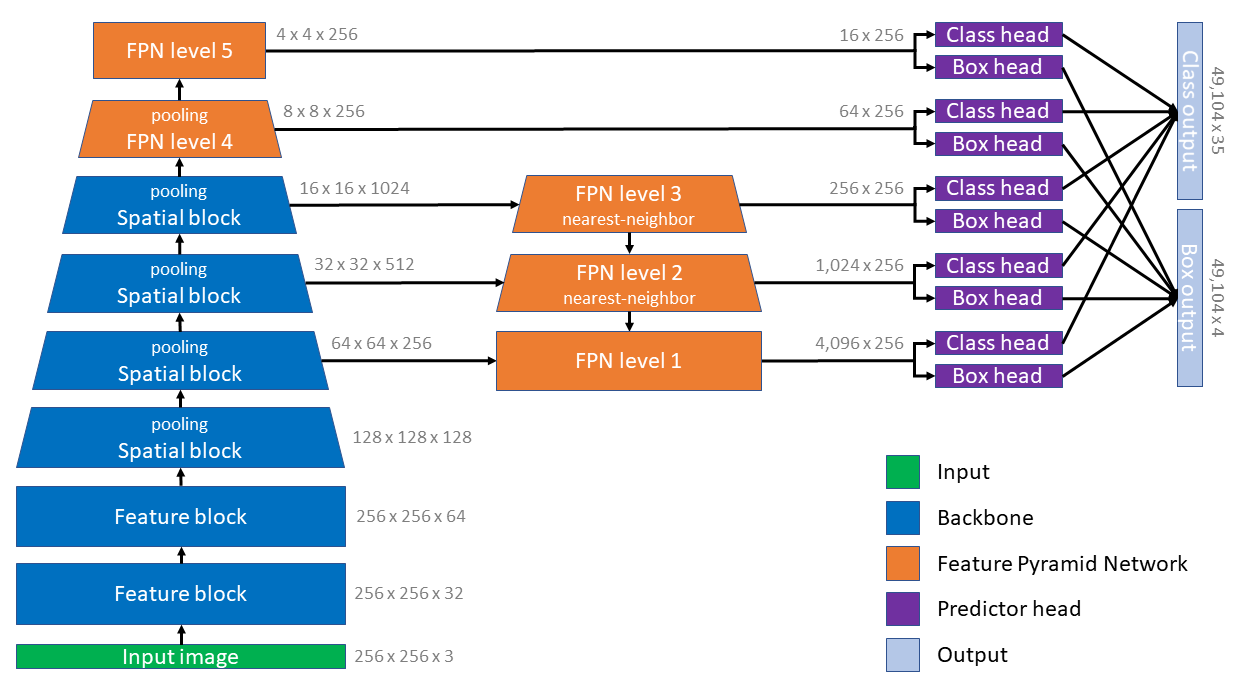
\includegraphics[width=1.0\columnwidth]{.//Figure/OCR/starter_detector.png}}
 \caption{The starter detector model. The predictor heads multiply the number of predictions by nine because of three different aspect ratios and three different scale ratios per anchor position.}
 \label{fig:starter_detector}
\end{figure}

\subsubsection{Loss and anchor configuration}

The default RetinaNet implementation uses anchor boxes of sizes \textit{32, 64, 128, 256, 512}. As the input images are only $256\times256$ pixels, I had to modify this. I used anchor boxes of sizes \textit{16, 32, 64, 128}, and \textit{256}. Similarly to the original configuration, I used three different aspect ratios \((\frac{1}{2}, \textit{1, 2})\) and three scale ratios \((\textit{0}, \frac{1}{3}, \frac{2}{3})\) for each anchor box size. With this configuration, the model had 49,104 anchor boxes for $256\times256$ inputs. The smallest anchor box the model can find is 16 pixels wide or long. This is \(\frac{1}{16}\)th of the input size. I consider it small enough because the input image is a license plate snippet, roughly 10-14 times as wide as one character on it. Thanks to the scale ratio, slightly smaller boxes can still be detected.

The models did not output any box prediction at the first few training sessions. It turned out that the loss function needed other parameters. The first problem was that the localization loss dominated the total value: there are 36 different classes in the OCR task, but the original COCO dataset has 80. An erroneous classification is more severely penalized if there are more classes by focal loss. I multiplied the localization penalty by 0.6 for downscaling. The other problem was that values for well-classified samples and wrongly empty-classified ones were very similar. The models learned to output nothing, thus minimizing the error. I tried different values to widen this gap and chose 0.85 and 1.2 for alpha and gamma parameters (instead of the original 0.25 and 2.0). After these modifications, the models could learn predicting boxes.

\subsubsection{Backbone}

I wanted to use as small network as possible. I tried a backbone with four convolutional layers as a starting point. This model could only localize huge boxes properly. This was because two convolutional layers could not generate a feature map that could be used to localize and classify objects. As I increased the number of layers, the detector got better. I added two feature blocks with one convolutional layer at the beginning of the network. After four layers, the starter model could output proper predictions (the last feature map responsible for huge objects). Increasing the number of layers helped the model converge, but the number of parameters got huge: I constrained the maximum output feature map in 512 dimensions to keep it low. In my opinion, this amount was enough to distinguish 36 classes properly.

I tried different feature map dimensions in the first convolutional layer; this value is then doubled for each block. The dimensions were \textit{16, 32}, and \textit{64}. The best results were with the value 32, but a model with only a 16-dimensional feature map produced similar results. Since this value significantly affects the size of the network, I chose the lowest because the deeper feature maps did not substantially affect performance as shown in Table \ref{tab:1st_feature_dimensions}.

\begin{table}[htb]
\caption{Detectors with different 1st layer feature dimensions.}
\label{tab:1st_feature_dimensions}
\noindent
\centering
\begin{tabular*}
{\columnwidth}{@{\extracolsep{\stretch{1}}}*{3}{r}@{}}
    1st feature map dimension & epochs & loss\\ \hline
    16 & $22$ & $1.4052$ \\
    32 & $26$ & $\textbf{1.4026}$ \\
    64 & $28$ & $1.4112$ \\         
\end{tabular*}
\end{table}

Next, I tried different feature map dimension constraints because this greatly influences the number of parameters. I experimented with values \textit{512, 256}, and \textit{128}. Training a model with 256 maximum feature dimensions did not decrease performance, but the model with only 128 could not achieve the same error rate. Hence, I chose 256 as the upper limit.

\subsubsection{Shift-invariance}

Initially, I used all the models with max-pooling. I experimented with the custom implemented blur-pooling layers, which worsened the performance in this case. I don't know the exact reason of this, but it could probably be that the feature edges of different objects got too blurred. This was not a problem with sequential models, where a character usually triggered multiple parts in a sequence, which CTC loss could handle. In object detection, it caused trouble in object localization. Therefore, I used max-pooling in the following models. Figure \ref{fig:blur_vs_max_pool} shows the effect of different pooling layers applied to an image containing larger objects.

\begin{figure}[htb]
 \centerline{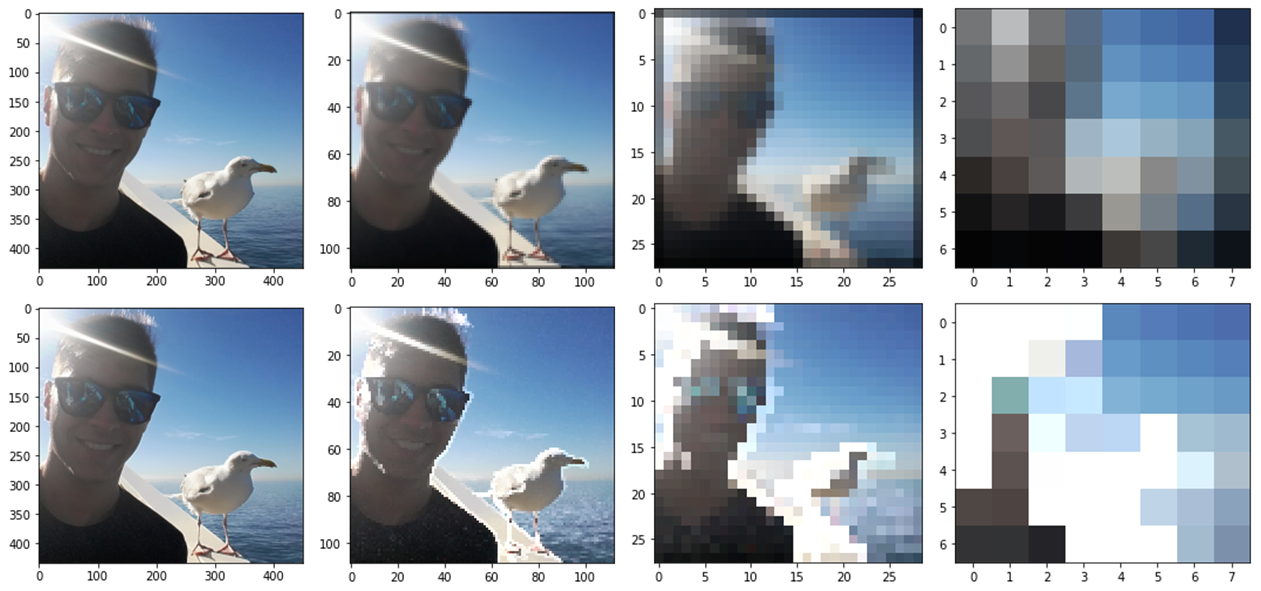
\includegraphics[width=1.0\columnwidth]{.//Figure/OCR/blur_vs_max_pool.png}}
 \caption{The effect of different pooling layers. The two variants were applied to the same $900\times865$ image eight times. The 2nd, 4th, 6th, and 8th downscaled images are shown. Blur-pooling was used with kernel size three and stride two (top) and max-pooling with stride two (bottom).}
 \label{fig:blur_vs_max_pool}
\end{figure}

\subsubsection{Predictor heads}

My implementation uses decoupled classifier- and localizer heads to produce the network output. I experimented with different input feature dimensions (coming from the FPN) and the number of layers.

I tried the predictor head input dimensions of \textit{256, 128}, and \textit{64}. The highest value matches the maximum dimensionality in the CNN backbone. Lower values can be interpreted as a feature downscaling in the FPN. Value 128 was the best choice because it could produce the best error rate in pair with dimension 256, leading to a significantly smaller network. Dimension 64 was too few for this problem. Table \ref{tab:predictor_head_dimension} summarizes the results.

\begin{table}[htb]
\caption{Comparison of predictor heads with different input dimensions.}
\label{tab:predictor_head_dimension}
\noindent
\centering
\begin{tabular*}
{\columnwidth}{@{\extracolsep{\stretch{1}}}*{3}{r}@{}}
    input dimension & epochs & loss\\ \hline
    64 & $22$ & $1.9347$ \\
    128 & $26$ & $\textbf{1.4033}$ \\
    256 & $28$ & $1.4052$ \\             
\end{tabular*}
\end{table}

RetinaNet uses two inner convolutional layers in the predictor heads before the last one reshaping the features to the output. I tried one, two, and three inner layers. A single layer was not enough. The loss was higher than with the other two approaches. The deepest predictor heads performed similar, but I chose the ones with two inner layers because of the similar performance but lower number of parameters. Results can be seen in Table \ref{tab:predictor_head_layers}.

\begin{table}[htb]
\caption{The effect of different number of inner predictor head layers on performance.}
\label{tab:predictor_head_layers}
\noindent
\centering
\begin{tabular*}
{\columnwidth}{@{\extracolsep{\stretch{1}}}*{3}{r}@{}}
    number of inner layers & epochs & loss\\ \hline
    1 & $20$ & $1.4456$ \\
    2 & $26$ & $1.4033$ \\
    3 & $22$ & $\textbf{1.3967}$ \\
\end{tabular*}
\end{table}

Sample inference results of the best model can be seen in Figure \ref{fig:inference_detector}. False positive predictions mainly cause the error. In the output processing, I used the Combined NMS algorithm with an IoU value of 0.5. To solve the false positive phenomenon, I could use the original NMS. Still, in that case, rotated images are likely to produce IoU values greater than the threshold among different objects, which carry the risk of dropping true positive objects close to each other. 

The TensorFlow Object Detection API model runs in 80 ms, while the proposed model's inference time is 317 ms. This phenomenon is caused by several things. The first is the number of anchor boxes. The API model uses around 12,000 anchor boxes, while the own implementation has four times more. This is because small anchor boxes are needed to detect small characters, drastically increasing the number of anchors. The other reason is that my implementation reuses the same predictor heads across different feature levels on the computational graph, leading to a smaller network size but longer inference time.

A development option could be to implement a YOLO-like detector, which uses objectness score to handle class imbalance, thus using a simpler, less parameter-sensitive loss function. Also, implementing an anchor-free version of the model could speed up inference time because the output tensor with roughly 50,000 items is a performance bottleneck. The model size can also be sacrificed using separate predictor heads for each feature level for better runtime.

\begin{figure}[htb]
 \centerline{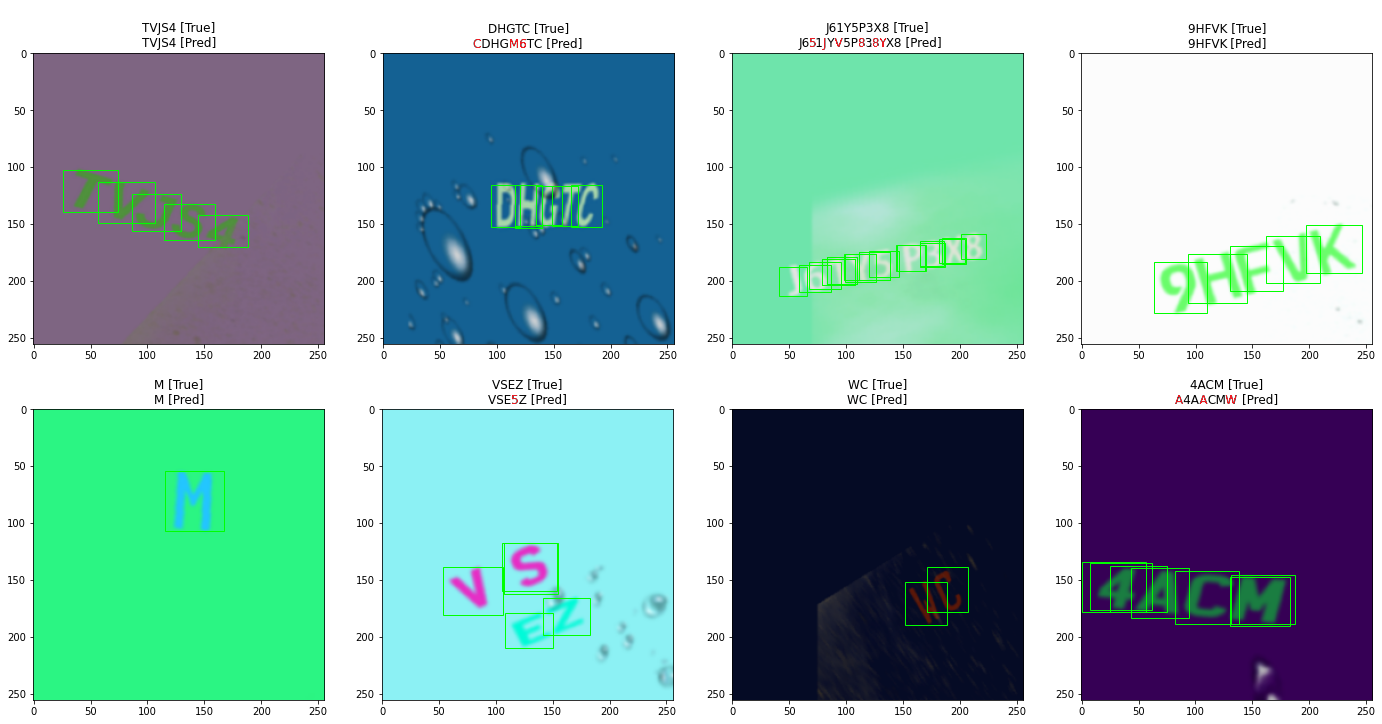
\includegraphics[width=1.0\columnwidth]{.//Figure/OCR/inference_detector.png}}
 \caption{Inference results of the best performing network. Incorrect detections are marked as red.}
 \label{fig:inference_detector}
\end{figure}

\section{Comparison}

This chapter provided a solution for the OCR task with both the sequential- and object detection approach. The sequential model is fast and simple but cannot process multiline texts efficiently. Object detection can handle them easily but requires roughly 2-3 times more parameters. However, its most significant problem is the inference time. With an anchor-free approach, the detector can be significantly faster, with which it can approach the runtime of the RCNNs. This is a future development opportunity. However, the present anchor-based detector is an order of magnitude slower than the sequential model, and more error prone due to the false positive predictions, so I chose the RCNN approach. The comparison of the two models can be seen in Table \ref{tab:sequential_detection_OCR_models}.

\begin{table}[htb]
\caption{Comparison of sequential and object detection OCR models.}
\label{tab:sequential_detection_OCR_models}
\noindent
\centering
\begin{tabular*}
{\columnwidth}{@{\extracolsep{\stretch{1}}}*{6}{r}@{}}
	model & host & input & parameters & size [KB] & inference [ms]\\ \hline
	sequential & CPU & 50x500x3 & $1,325,734$ & $639$ & $37$ \\
	object detection & CPU & 256x256x3 & $3,557,484$ & $4,541$ & $317$ \\
\end{tabular*}
\end{table}
%----------------------------------------------------------------------------
\chapter{System Overview}

In this chapter, I overview the complete system. I explain the main design decisions, and some more exciting implementation details.

\section{ALPR pipeline}

The applied pipeline is shown by Figure \ref{fig:pipeline}. It compresses the traditional tasks into as few steps as possible. The structure is like the one used in WPOD-NET\cite{WPOD-NET}, with some differences. First, a RetinaNet\cite{RetinaNet} detector is used for both vehicle and plate localization (instead of a YOLOv2\cite{YOLOv2} vehicle-only detector). The rectification step is excluded from our pipeline, which is a drawback in plate image quality. However, WPOD-NET's rectification supports only one plate scale, so adding it would not be a general solution, in our opinion. On the other hand, it would increase the computational load as it must run separately for each detected vehicle. The second step is to filter possible plate objects based on location and confidence scores. The third is to cut plate objects from the original image.

\begin{figure}[H]
 \centerline{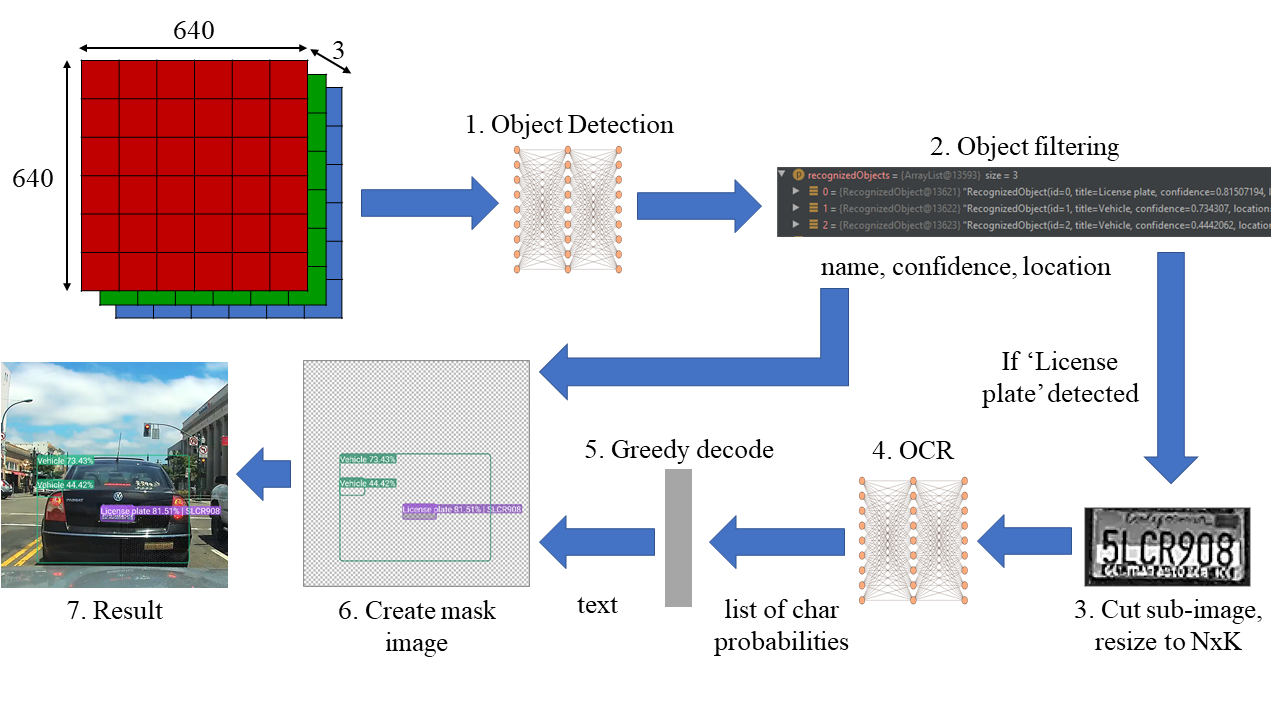
\includegraphics[width=1.0\columnwidth]{.//Figure/System/pipeline.png}}
 \caption{The applied ALPR pipeline.}
 \label{fig:pipeline}
\end{figure}

The pipeline models are dynamically quantized TensorFlow Lite converted networks. On a Samsung Galaxy S10 smartphone, where an image contains only one license plate, the average runtime is roughly 160 ms. The processing steps are as follows:

\begin{itemize}
  \item image preprocessing (9 ms)
  \item detector inference (75 ms on GPU)
  \item cutting and resizing the license plate image segment (3 ms)
  \item OCR inference (37 ms on CPU)
  \item Greedy decoding (<1 ms)
  \item creating mask image (33 ms)
\end{itemize}

This runtime may change depending on the number of plates on a picture, as the OCR steps must be repeated on each license plate image segment.

Table \ref{tab:OCR_model_runtimes} summarizes the runtimes of different OCR models. Besides the best-performing network, I also tested the initial architecture (batch 128). It runs in 37 ms on the device's GPU. Keeping in mind the runtime, it is worth sacrificing marginal quality (+\({9.5} \times {10^{-3}}\) loss) to acquire a $1.5\times$ speed-up. As a reference, Google's MLKit Vision Text Recognizer\cite{MLKitTextRecognition} runs in 40 ms on the same plate image with a single line of text. The MLKit model is a multiblock recognizer. However, when more than one block is present, its runtime increases drastically.

\begin{table}[htb]
\caption{Running time in milliseconds for OCR models.}
\label{tab:OCR_model_runtimes}
\noindent
\centering
\begin{tabular*}
{\columnwidth}{@{\extracolsep{\stretch{1}}}*{6}{r}@{}}
    model & host & input & size [KB] & loss & inference [ms]\\ \hline
    batch 128 & CPU & 50x500x3 & $639$ & $0.0848$ & $37$ \\
    MLKit & CPU & 50x500x3 & $?$ & $?$ & $40$ \\
    batch 128 & GPU & 50x500x3 & $639$ & $0.0848$ & $50$ \\
    Hyper1st & CPU & 50x500x3 & $4,447$ & $0.0753$ & $56$ \\
    MLKit & CPU & 200x200x3 & $?$ & $?$ & $72$ \\
    Unfolding & CPU & 200x200x3 & $3,133$ & $0.0991$ & $221$ \\
    Unfolding & GPU & 200x200x3 & $3,133$ & $0.0991$ & $372$ \\
\end{tabular*}
\end{table}

\section{Frontend}

The client application's main task is to detect stolen vehicles, then report them using location and time data. The application runs the pipeline on the device, and it is possible to run an evaluation on loaded images and the live image feed. The user constantly sees what has been recognized. Stolen vehicle and user data are stored in a local SQLite database, synchronized in the background with the API. Available camera operations include front/back camera switching, image saving, tap to focus, and pinch to zoom. I present the Android application's architecture and some details in the following.

The application can receive inputs from two different sources. The first option is to load an image from the storage. In this case, the image is processed only once, and the meta-information (GPS location, UTC timestamp) is extracted from the image's Exif (Exchangeable image file format) content. This format is supported by almost any type of smartphone (if not, fallback values are used, which cannot be reported to the server). This is important because otherwise, a stolen vehicle image from the past could overwrite a more recent recognition on the server when reporting the match. The other option is to process the live camera feed. For this, the current camera frame is fed into the pipeline. When the results are ready, the current live frame is processed, meaning that frames are discarded while the pipeline is processing. The live feed results are accompanied by the device's location and system UTC timestamp information. If they are unavailable, fallback values are used. In both cases, image preprocessing steps are applied shown by Figure \ref{fig:image_preprocessing}. Some images of the application are shown in Figure \ref{fig:AppImages}.

\begin{figure}[htb]
 \centerline{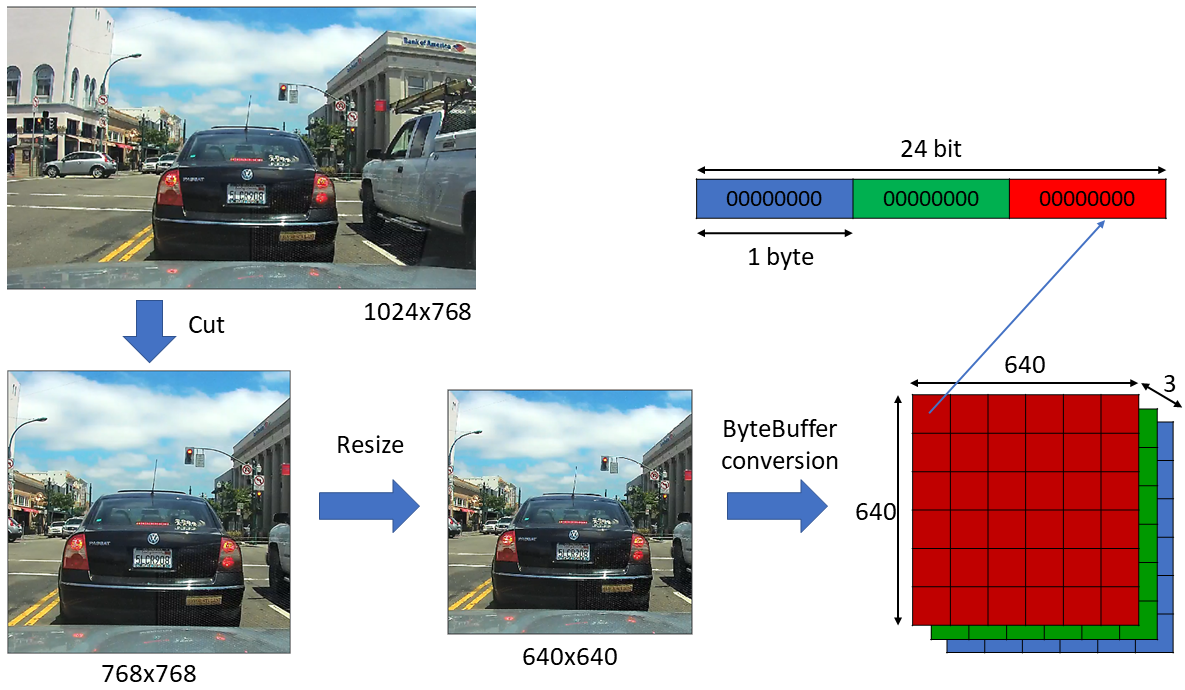
\includegraphics[width=0.9\columnwidth]{.//Figure/System/image_preprocessing.png}}
 \caption{Image preprocessing steps before feeding the pipeline.}
 \label{fig:image_preprocessing}
\end{figure}

\begin{figure}[H]
 \centerline{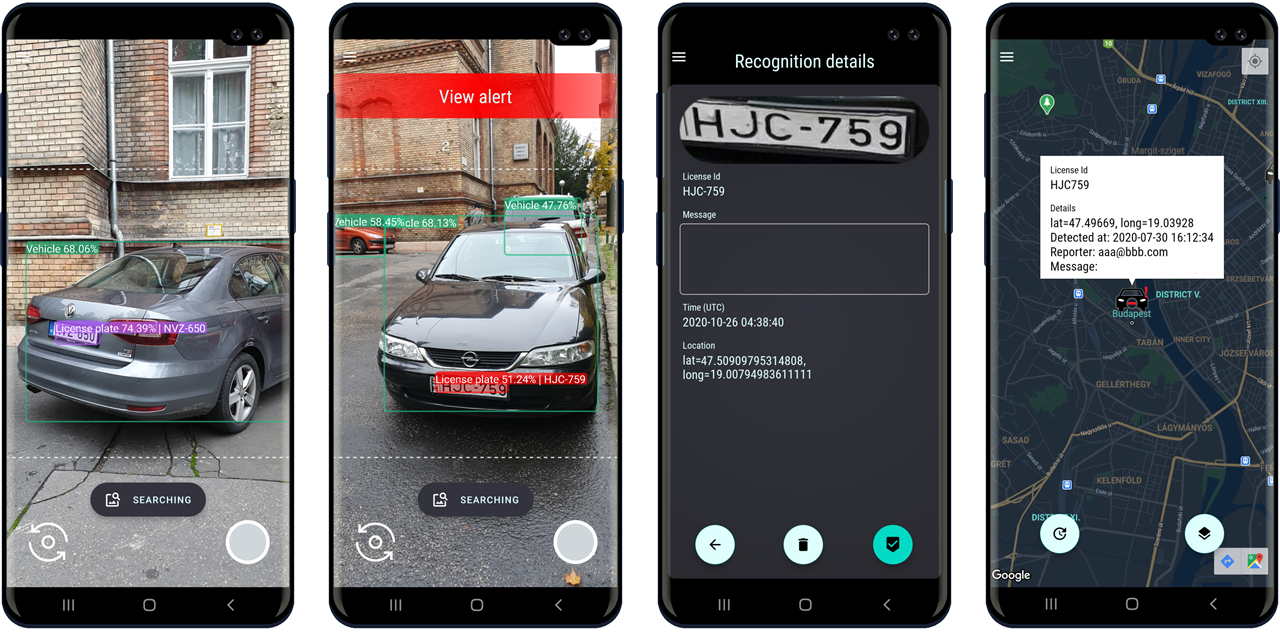
\includegraphics[width=1.0\columnwidth]{.//Figure/System/AppImages.png}}
 \caption{Live feed recognition (1st screen) and an identified stolen vehicle (2nd screen). Details can be inspected and a message can be added to a recognition (3rd screen). When a vehicle is reported, its last known position is visible on the map (4th screen).}
 \label{fig:AppImages}
\end{figure}

\subsection{Architecture}

I used the \textit{Model View ViewModel} (MVVM) UI design pattern. It is an event-driven model invented by Microsoft to take advantage of data binding capabilities. In MVVM, the View contains UI descriptive code often in a declarative (XML, XAML, HTML) form, and the connection to the ViewModel is realized with explicit data binding. Therefore, there are fewer classic coding tasks in Views, and the business logic components can be easily separated.

There are sub-layers in the model level of the application. I explain the hierarchy through the steps of reporting a single item. Suppose a new stolen vehicle was detected on the live camera feed, and the user selected to report it. In this case, the user sees a ReportActivity, which has a ViewModel storing the UI state. The report item gets stored in a list wrapped in a LiveData object (observable from the Activity). When the user clicks on the send button, the related data is transmitted to the RepositoryService in the model layer. Inside this service, there is the ReportRepository. It hides further data operations (database handling, API communication) from the outside. When it receives a new report, it transforms it into a format stored in the Report table and persists with ReportDAO (data access object) to the database. After that, it calls ApiService to send the report to the server. When the response arrives from the API, ReportRepository updates the corresponding item in the database. Until the operation is unsuccessful, the user sees the report as pending. Pending items can be deleted or re-sent at any time. Figure \ref{fig:AndroidArchitecture} shows a high-level overview of the sub-layers and modules.

\begin{figure}[htb]
 \centerline{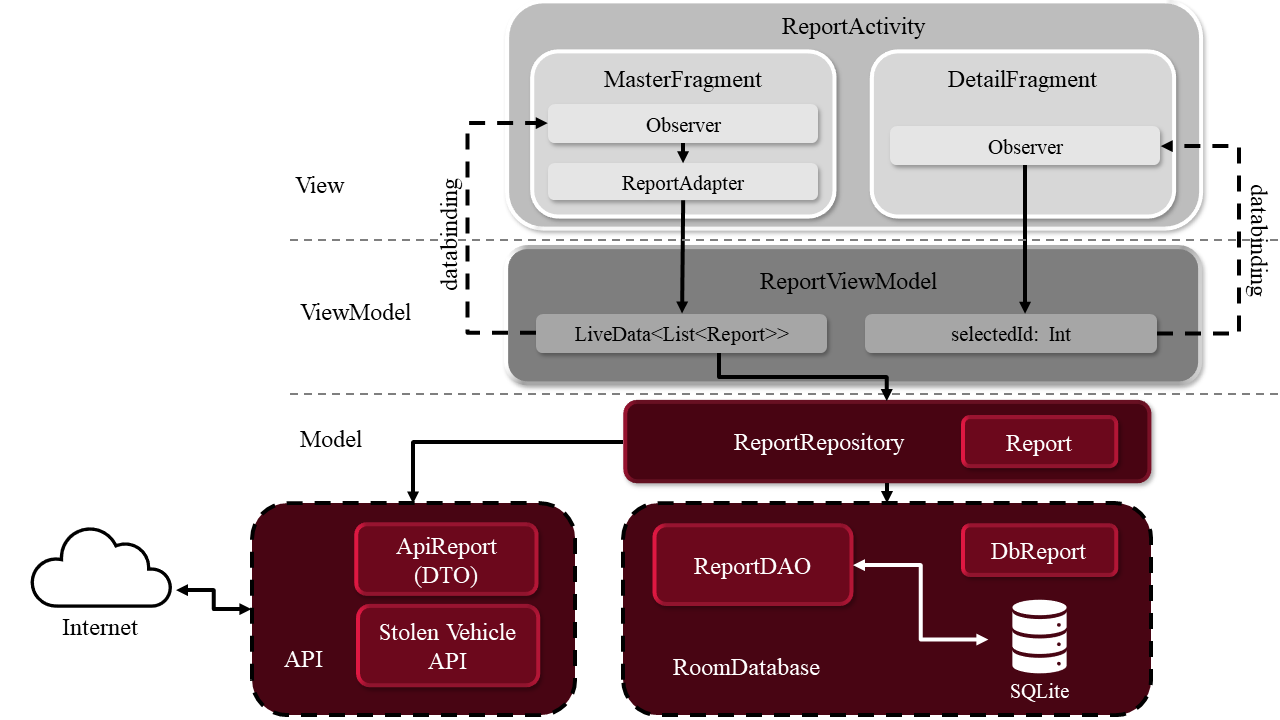
\includegraphics[width=1.0\columnwidth]{.//Figure/System/AndroidArchitecture.png}}
 \caption{MVVM layers in the application.}
 \label{fig:AndroidArchitecture}
\end{figure}

\newpage
\subsection{Database}

Beyond reports, the application stores several other information in its local relational database (list of stolen vehicles, account information, metadata). Outside the relational database, the application stores user preferences as key-value pairs. The complete database schema can be seen on Figure \ref{fig:AppData}. The persisted data schema differs from the in-memory data representation in order to be independent of higher-level modules. The schema of the data transfer objects (DTOs) is different for the same reason. This way, in case of API- or database schema changing, only the corresponding module needs to be updated, resulting in maintainable code.

\begin{figure}[H]
 \centerline{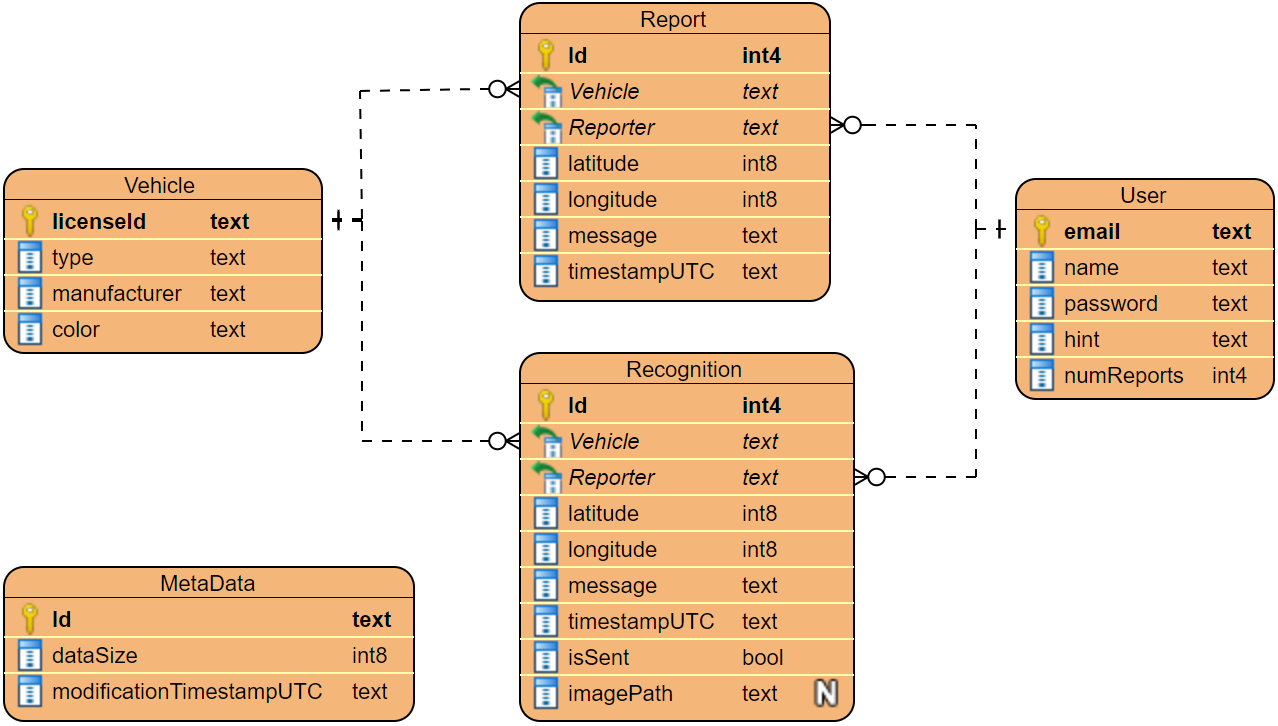
\includegraphics[width=1.0\columnwidth]{.//Figure/System/AppData.png}}
 \caption{Client application database schema.}
 \label{fig:AppData}
\end{figure}

\subsection{Vulnerabilities}

I would like to draw attention to some vulnerabilities of the application. By manipulating the Exif information of an image (changing coordinates, setting a timestamp to a later time), false recognition can be uploaded to the server, which can overwrite the current vehicle position record. Unfortunately, there is no robust solution to detect whether an image's Exif content has been modified or not by the time of this work. Also, an image editor can easily edit a recent photo (with valid Exif information) to contain a stolen vehicle in it. When using the live camera feed, pointing to an image of a stolen vehicle can also trigger a false report. These are opportunities for abuse due to the nature of image-based recognition. To prevent them, images inducing the report could also be uploaded to the server for further inspections. When a report's metadata is fallback or invalid, the application refuses to send them to the server.

\newpage
\section{Backend}

The server application provides the API for the clients and manages registered users. It has a stateless REST API, so a user needs to authenticate itself when querying the server.

\subsection{Architecture}

The server has a three-layered architecture (Figure \ref{fig:ServerStructure}). Because it is responsible for API service and data storage, it does not have a separate View layer (only a simple web-based UI is available). Instead of the UI layer, the communication layer through which the API services can be accessed. It is loosely coupled with other layers. User authentication is done with HTTP basic authentication. In the business logic layer, the Authenticator module checks requests and does not allow them to be executed when the required permissions are missing. The Interactor contains the main business logic. The data access layer contains the DAO classes responsible for handling their tables and providing a unified interface for retrieving/writing data.

\begin{figure}[htb]
 \centerline{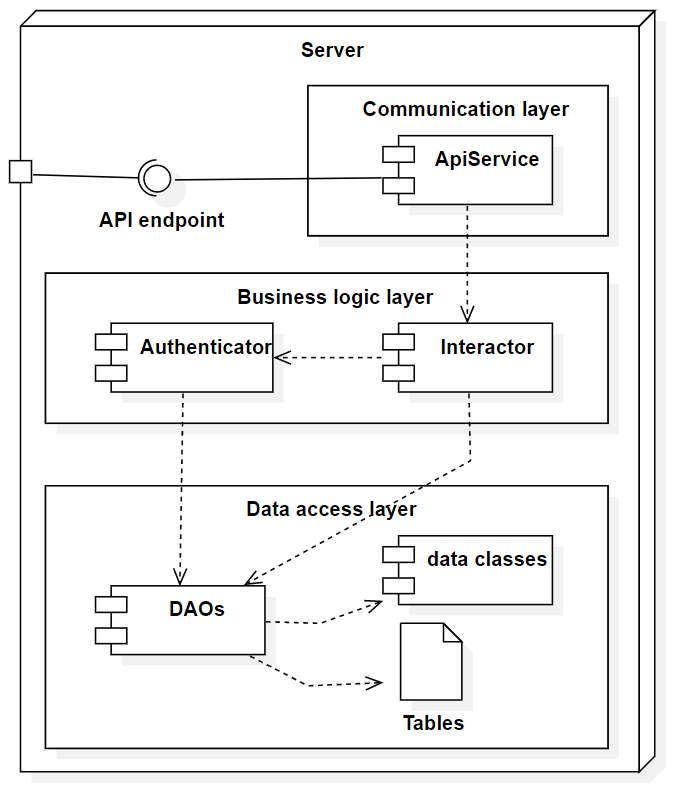
\includegraphics[width=0.5\columnwidth]{.//Figure/System/ServerStructure.png}}
 \caption{Structure diagram of the server.}
 \label{fig:ServerStructure}
\end{figure}

\subsection{Database}

Since I decided to use a self-created database, I briefly describe its main guidelines. It is a NoSQL variant with an in-memory approach. The tables store information in an object-oriented manner. The table contents are in JSON format (like in the case of MongoDB). The server uses the Gson library to encode and decode JSON files. Figure \ref{fig:ServerData} represents the schema of the stored objects.

There are tables of stolen vehicles, current reports, and user accounts. To these contents, history files(write only) are available. They store all items using a timestamp and a version number to support recovery and traceability. History tables are not stored in memory, and when a data table is updated, its corresponding history is automatically updated. There is a meta content storing size and timestamp information of the previous tables. Lastly, an Event table records system logs (also write-only).

The database serves requests from memory, making API responses fast because there is no need to wait for I/O operations. The memory content is synchronized with the corresponding table in the background. It is a viable solution as too many data records are never stored on the server (the images are not uploaded). I examined the most significant JSON object type (report) to validate this. One record takes up 173 bytes in the memory. The server needs 173 MB memory when 1 million records exist. It is a severe overestimation, though, as the stolen vehicles list obtained by web scraping typically has just a few thousand items (in the case of Hungary). That is the maximum number of records that the in-memory database ever has (when every stolen vehicle was detected). As the history content is stored persistently, extensive API usage neither saturates the memory. Given the scalability of the database, one server instance could handle all European countries.

\begin{figure}[htb]
 \centerline{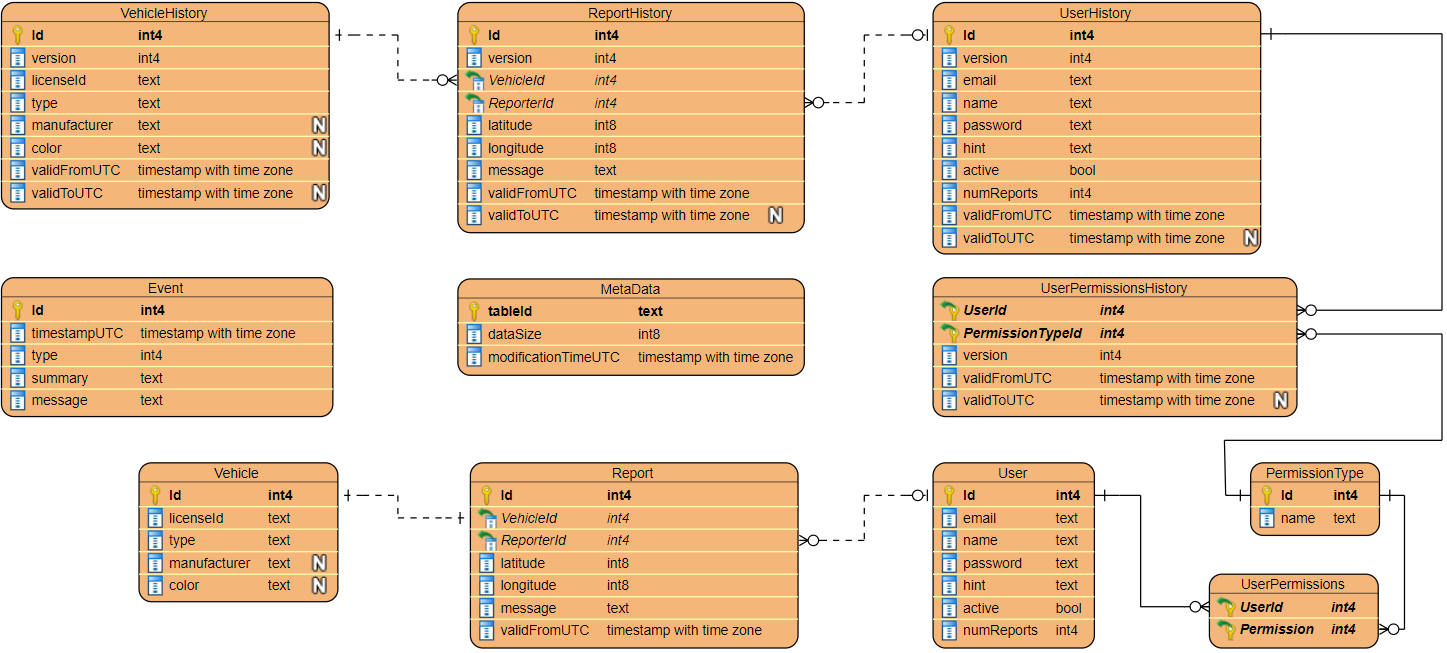
\includegraphics[width=1.0\columnwidth]{.//Figure/System/ServerData.png}}
 \caption{Server data schema.}
 \label{fig:ServerData}
\end{figure}

\subsection{API}

The API is divided into five parts: \textit{Vehicles, Reports, Report history, Self}, and \textit{Users}. These names are also the corresponding endpoint prefixes. All query endpoints have similar actions and a unified calling convention. All actions are subject to specific permissions, evaluated before serving. There is also a status page describing the API and its interface.

\subsection{Permission}

The nature of stored data (location and timestamp of stolen vehicles) could potentially allow abuses, so there is an allowlisting role-based permission model. Users with specific roles are eligible to execute various operations. There are ADMINISTRATOR, API\_REGISTER, SELF\_MODIFY, API\_GET, and API\_SEND permissions. Users can be uniquely identified by their inner server Id or email address.

\begin{itemize}
\item API\_GET lets an authorized account query report.
\item API\_SEND makes it possible to send recognitions to the server.
\item SELF\_MODIFY is needed to prevent blocklisted users from deleting themselves and re-register.
\item An ADMINISTRATOR user can modify the server and any user's permissions at any time. If someone's behavior is suspicious, an administrator can revoke permissions, delete a user, or deactivate and blocklist it. An administrator can also register a new user with specific permissions.
\item The default user (e.g., client application users) has an account with an API\_REGISTER role. This way, it is possible for newcomers to register their new accounts. If someone tries to use the application without signing in, this user is utilized. The only API permission is registration. Although someone can detect vehicles on-device, they cannot report them or see current reports. This API\_REGISTER role prevents anyone outside of the client application from registering. The default user can create a new account with SELF\_MODIFY, API\_GET, and API\_SEND permissions.
\end{itemize}

\subsection{Vulnerabilities}

The server stores sensitive data so attempts to abuse should be considered. Passwords are stored on the server in an encrypted format. No one can access user passwords - although administrators can block or delete users. Data access is based on an allowlisting model, meaning that anything which is not explicitly allowed is forbidden. The sensitive API endpoints (user actions, data uploads, and queries) are only available through HTTPS communication. Every database access is through predefined functions with a predefined list of allowed parameters, meaning that injection attacks are not possible. Users outside the client application cannot register, as the front-end contains a protected default user solely used to register new accounts. 

If the attacker is an inner user, its behavior can be monitored: if there are too many reports from the same account, or the report locations/timestamps are suspicious, administrators can revoke the API\_SEND permission or even block the user. When an account is blocked, it cannot query or upload. A blocked user cannot delete itself or re-register, meaning that it cannot access the server with the same email address anymore. If a badly-formatted report is received, the server discards it. If the report's metadata is invalid (non-existing GPS coordinates, future UTC timestamps), the server also discards it. If an attacker is an administrator, it can delete the current database state. However, the state can always be restored with the help of the history content, which cannot be deleted. Administrators cannot access other users' sensitive content (although they can delete accounts). Other administrators can block an administrator.
%----------------------------------------------------------------------------
\chapter{Summary}

In my thesis, I discussed the general task of Automatic License Plate Recognition, then examined best practices for both Object Detection and Optical Character Recognition. I trained deep learning based models to detect number plates and recognize texts on them, then a full ALPR pipeline has been created. Then, I integrated my solution into a stolen vehicle identification system. In the end, I presented the key concepts of my system's frontend and backend applications.

Further work would focus on the license plate detection step, which could be optimized by using better models in detecting small objects like Ultralytic's YOLOv5\cite{YOLOv5}. Using a detector that recognizes rotated rectangular coordinates could eliminate the need for plate rectification (which the current pipeline lacks); therefore, using a WPOD-NET-like network should also be considered.

% Acknowledgements
%~~~~~~~~~~~~~~~~~~~~~~~~~~~~~~~~~~~~~~~~~~~~~~~~~~~~~~~~~~~~~~~~~~~~~~~~~~~~~~~~~~~~~~
%----------------------------------------------------------------------------
\chapter*{\koszonetnyilvanitas}\addcontentsline{toc}{chapter}{\koszonetnyilvanitas}
%----------------------------------------------------------------------------

The author would like to express his thanks to D\'aniel P\'asztor for his valuable support as a scientific advisor. The work presented in this paper has been carried out in the frame of project no. 2018-1.1.2-KFI-2018-00062, which has been implemented with the support provided by the National Research, Development and Innovation Fund of Hungary, financed under the 2018-1.1.2 KFI. funding scheme. It was also supported by the BME Artificial Intelligence TKP2020 IE grant of NKFIH Hungary (BME IE-MI-SC TKP2020) and by the Ministry of Innovation and the National Research, Development, and Innovation Office within the framework of the Artificial Intelligence National Laboratory Programme.


% List of Figures, Tables
%~~~~~~~~~~~~~~~~~~~~~~~~~~~~~~~~~~~~~~~~~~~~~~~~~~~~~~~~~~~~~~~~~~~~~~~~~~~~~~~~~~~~~~
%\listoffigures\addcontentsline{toc}{chapter}{\listfigurename}
%\listoftables\addcontentsline{toc}{chapter}{\listtablename}


% Bibliography
%~~~~~~~~~~~~~~~~~~~~~~~~~~~~~~~~~~~~~~~~~~~~~~~~~~~~~~~~~~~~~~~~~~~~~~~~~~~~~~~~~~~~~~
\addcontentsline{toc}{chapter}{\bibname}
%\bibliographystyle{unsrt}
\bibliography{bib/citings}


% Appendix
%~~~~~~~~~~~~~~~~~~~~~~~~~~~~~~~~~~~~~~~~~~~~~~~~~~~~~~~~~~~~~~~~~~~~~~~~~~~~~~~~~~~~~~
%%----------------------------------------------------------------------------
\appendix
%----------------------------------------------------------------------------
\chapter*{\fuggelek}\addcontentsline{toc}{chapter}{\fuggelek}
\setcounter{chapter}{\appendixnumber}
%\setcounter{equation}{0} % a fofejezet-szamlalo az angol ABC 6. betuje (F) lesz
\numberwithin{equation}{section}
\numberwithin{figure}{section}
\numberwithin{lstlisting}{section}
%\numberwithin{tabular}{section}


%\label{page:last}
\end{document}
